\documentclass[12pt]{article}
\usepackage[english]{babel}
\usepackage[utf8]{inputenc}
\usepackage{amsmath}
\usepackage{graphicx}
\usepackage{float}
\usepackage[colorinlistoftodos]{todonotes}
\usepackage[bottom=1in,top=1in,right=1in,left=1.5in,]{geometry}
\usepackage{setspace}
\doublespacing
\usepackage[lofdepth]{subfig}
\usepackage{graphicx}
\usepackage[nottoc]{tocbibind}
\usepackage{titletoc}
\usepackage[toc,page]{appendix}
\usepackage[sectionbib]{natbib}
\usepackage{multirow}
\usepackage{courier}
\usepackage{listings}
\usepackage{color}
\usepackage{hyperref}

\definecolor{codegreen}{rgb}{0,0.6,0}
\definecolor{codegray}{rgb}{0.5,0.5,0.5}
\definecolor{codepurple}{rgb}{0.58,0,0.82}
\definecolor{backcolour}{rgb}{0.95,0.95,0.92}

\lstdefinestyle{mystyle}{
	commentstyle=\color{codegreen},
	keywordstyle=\color{magenta},
	numberstyle=\tiny\color{codegray},
	stringstyle=\color{codepurple},
	basicstyle=\footnotesize\ttfamily, %\small
	breakatwhitespace=false,         
	breaklines=true,                 
	captionpos=b,                    
	keepspaces=true,                 
	numbers=left,                    
	numbersep=5pt,                  
	showspaces=false,                
	showstringspaces=false,
	showtabs=false,                  
	tabsize=2
}

\lstset{style=mystyle}

\begin{document}
\pagenumbering{gobble}
\

\begin{center}
	\uppercase {Big data analysis of futures: Penalized Regression Splines for trade Volume Prediction and Price Volatility vs trade volume relationship}\\
	\vspace{1in}
	by\\
	Aniver Oluwatobi Bosede\\
	\vspace{1.5in}
	A thesis submitted to Johns Hopkins University in conformity with the requirements for the degree of Master of Science in Engineering\\
	\vspace{.5in}
	Baltimore, Maryland\\
	\vspace{2in}
	\copyright{} 2017 Aniver Oluwatobi Bosede\\
	All Rights Reserved
\end{center}
\newpage
\pagenumbering{roman}
\setcounter{page}{2}

\section*{Abstract}
\addcontentsline{toc}{section}{Abstract}
Whether an entity seeks to create trading algorithms or mitigate risk, predicting trade volume is an important task which comes with challenges, one of which is the sheer size of the data. In addition, meaningful insight that can be used to forecast price volatility using trade volume is often sought, as well as understanding of whether trade volume versus price volatility relationships support theories regarding market agents such as speculators and hedgers. This work focuses on futures trading and relies on Apache Spark for processing data spanning hundreds of millions of rows. It also utilizes a penalized spline regression approach to predict trade volume and assess which variables are most relevant. Finally, prior research claims regarding the correlation between trade volume and price volatility are investigated. The results serve to improve trader effectiveness and the regulation of futures markets.
\newpage

\section*{Acknowledgments}
\addcontentsline{toc}{section}{Acknowledgments}
%remember to acknowledge Naiman and Duncan 
I would like to acknowledge my awesome advisor, Professor Daniel Naiman for agreeing to voyage with me into the unknown world of cluster computing, and for his patience in the early stages of this work so that the compute environment could be configured, as well as ensuring the success of the arduous task of collecting the raw data.

Also, I would like to acknowledge the Acheson J. Duncan Fund for the Advancement of Research in Statistics for supporting this work.
 
\newpage

\tableofcontents
\newpage
\begingroup
\renewcommand\numberline[1]{}
\listoftables
\newpage
\listoffigures
\endgroup
\newpage

\pagenumbering{arabic}	
\setcounter{page}{1}
\section*{Introduction}
\addcontentsline{toc}{section}{Introduction}
%should i indent 1st paragraph? add stuff here about previous methods used such as GARCH, splinsDSC, and NueralNetworks?
Technology has advanced so far that in our society today we are constantly collecting data \cite{economist_10}. This has created the issue of how to feasibly analyze such overwhelming amounts of data \cite{economist_10}. We can then consider how to efficiently store it or how to best carry out statistical computations \cite{zaharia2016apache}. The aforementioned together form the relatively new and evolving field of big data. The research here focuses on the analysis of hundreds of millions of rows of futures trading data with the aid of Apache Spark (Spark). 

Spark is a fault-tolerant and general-purpose cluster computing system providing APIs in Java, Scala, Python, and R \cite{meng2016mllib}. Spark was chosen for the analysis over the similarly popular Hadoop MapReduce (MapReduce) because of Spark’s performance advantages as well as its greater computational capabilities \cite{zaharia2010spark}. Not only does Spark cache data resulting in persisted in-memory manipulations \cite{zaharia2012resilient}, it also includes Structured Query Language (SQL) and MLlib, a machine learning library \cite{meng2016mllib}. Conversely, MapReduce only does manipulations via disk reads and thus does not allow for data sharing \cite{zaharia2016apache}. Furthermore for a typical pipeline, external systems would have to be combined with MapReduce to provide querying and machine learning functionality \cite{zaharia2016apache}. In this case, 
a stand alone setup was employed, meaning that analysis was done using a one node cluster or one machine. Out of convenience the local file system was used for storage as opposed to a database like Cassandra or HDFS (Hadoop Distributed File System). However, for long term data analysis, it would be worthwhile to invest the time needed to set up a more robust data storage system. 

The futures trading data come from the Chicago Mercantile Exchange (CME) and were collected from May 2, 2016 to November 18, 2016. % only used from about May to September 
Raw data from the CME included extended hours trading and was collected via the Trading Technologies X\_TRADER® API RTD (Real Time Data) server. The server returned raw records with instrument name, maturity, date, time stamp, price, and quantity fields.
The futures were comprised of 21 financial instruments spanning six markets - foreign exchange, metal, energy, index, bond, and agriculture recording roughly a trade every half second. %/home/dnaiman1/findata/big_harvest/Trades_2016_11_18.csv
First, this work uses spline regression to predict the volume of trading for any given day. Volume during a particular time period is taken to mean the number of units traded. A spline regression was chosen due to lack of knowledge regarding the likely non-linear function underlying the response to covariates, in particular time to maturity. Predicting trade volume is of interest because many trading algorithms depend on volume \cite{satish2014predicting}.   Additionally, accurate volume predictions over a given interval allows traders to be more effective \cite{satish2014predicting}. In general, volume prediction increases trading strategy capacity, controls trading risk, and manages slippage \cite{satish2014predicting}.  

Second, the relationship between price volatility and trade volume is explored using standard deviation as a measure of volatility. In particular, volatility vs daily volume and volatility versus hourly volume were plotted to see whether or not the correlation remained the same with the passing of days and hours. It should be noted that unpredictable volume shocks have been known to be more predictive of change in volatility than predictable volume changes \cite{bessembinder1993price}.
%there is evidence suggesting that comparisons between volatility and total volume do not extract all information
This volatility-volume relationship is of importance due to the notion that hedgers are motivated to trade futures to stabilize their future income flows or costs, wherein the volume of their trading is based on their expectation of price variability \cite{foster1995volume}. Likewise, speculators are motivated to trade futures based on expectations of price variability \cite{foster1995volume}. Due to the fact that new information on the market causes agents such as hedgers and speculators to trade until prices reach a revised equilibrium, which then changes price and trading volume, we expect a positive correlation between volatility and volume \cite{foster1995volume}. Indeed past research indicates that there is a positive relationship between volume and price volatility \cite{foster1995volume}. This sort of exploration provides information on the efficiency of futures markets which regulators can then use to decide upon market restrictions \cite{foster1995volume}. 
%Talk about what futures are?

\section*{Methods}
\addcontentsline{toc}{section}{Methods}
A cubic regression spline was thought to be appropriate for modeling trade volume. Spline regression derives its name from a draftsman’s spline which is a flexible strip of metal or rubber used to draw curves \cite{harrell2015regression}. Similarly, spline basis functions are piecewise polynomials used in fitting curves which are linear in terms of the basis function. Splines have been used, principally in the physical sciences as well as in biomedicine, to approximate a wide variety of functions \cite{harrell2015regression}. Cubic splines in particular have been found to have nice properties with good ability to fit nonlinear curves. Cubic splines are made to be smooth at the knots, endpoints of intervals on the x-axis, by forcing the first and second derivatives of the function to agree at the knot \cite{harrell2015regression}.  

Holidays were removed from the raw data. Then the day of the month, day of the week, and hour of the trade were extracted from the time stamp. An aggregation was then done to sum the number of trades per hour for each product, where product is defined as an instrument-maturity pair. There were 139 such products. Aggregation reduced the data from 105 million records to 8,826 records. Day, time to maturity, and market fields were created and total trade volume for each day was calculated.

Exploratory analysis was then done on the reduced data set. To ensure that a spline regression was appropriate for modeling trade volume, the first thing done was to create histograms of the trade volumes. One of the assumptions behind regression is that the response conditioned on the predictors is normally distributed. Even if normality fails, regression can be an effective tool, but under normality least squares is optimal. Thus transforming to normality is desirable. The histogram of the raw trade volume was skewed as shown in left of Figure 1. Therefore the volume was Box-Cox transformed, after which the data became normal as shown in right of Figure 1.

\begin{figure}[H]
	\begin{center}
	\begin{tabular}{cc}
		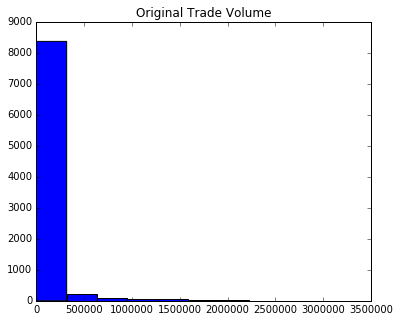
\includegraphics[width=6.5cm]{hist_orig.png}
		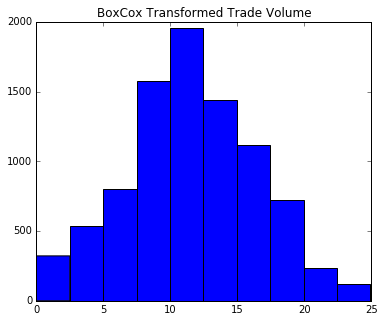
\includegraphics[width=6.25cm]{hist_bc.png}
	\end{tabular}
	\caption{Histograms of  trade volume before and after Box-Cox transform}
	\label{fig:dum1}
	\end{center}
\end{figure}

There was curiosity regarding how trade volume changed as time passed. Thus a plot of the transformed trade volume versus day ignoring weekends was made. Referring to the left plot in Figure 2, the trade volume appears constant across the days with a cluster of high volume trades above 20, which untransformed is 412,823 trades. This is almost half a million trades of a single product in a single day.

Also intuitively, it makes sense that less trading occurs far from maturity and near maturity. Far from maturity speculators might not have any information that would move them to purchase a future and most hedgers may only seek to minimize risk in the short term. Then near maturity traders are closing their positions. To confirm 

\begin{figure}[H]
	\begin{center}
		\begin{tabular}{cc}
			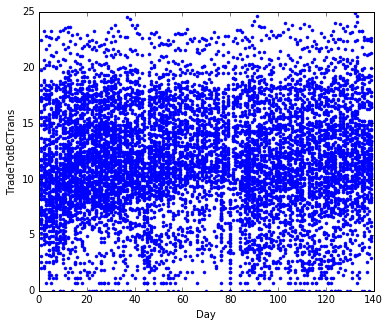
\includegraphics[width=6.5cm]{bc_sample_day_wMat.png}
			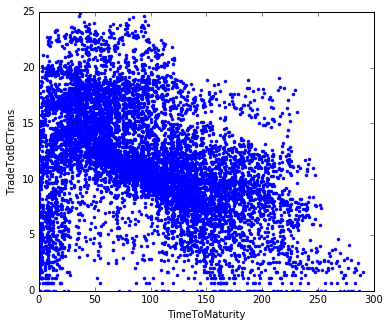
\includegraphics[width=6.5cm]{time_to_mat.png}
		\end{tabular}
		\caption{Plot of trade volume as days pass and as time to maturity gets further.}
		\label{fig:1}
	\end{center}
\end{figure}

\noindent this theory a plot was made of the transformed trade volume versus time to maturity, right in Figure 2. Looking at the plot it appears that the data follows intuition. 
 
\begin{figure}[H]
	\begin{center}	
		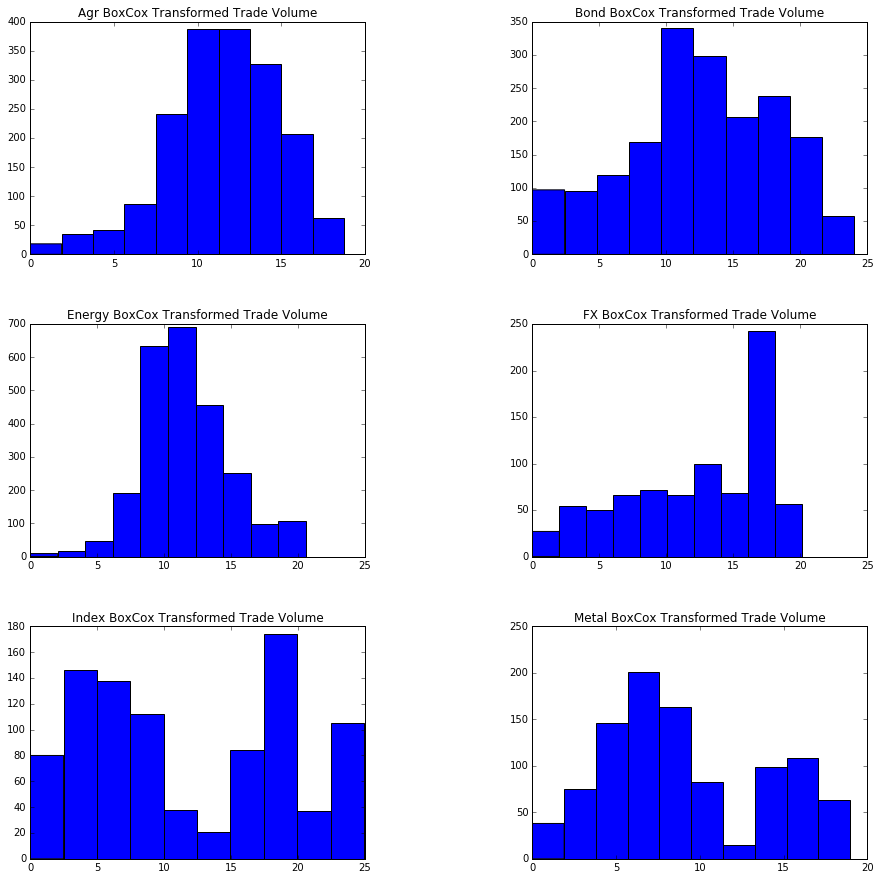
\includegraphics[width=15cm]{types_bc_hist.png}
		\caption{Histograms for instrument types}
		\label{fig:2}
	\end{center}
\end{figure}
Whether it made sense to make one model or several models for each instrument market: foreign exchange, metal, energy, index, bond, and agriculture was also considered. This would mean that each of the markets need to have near normal distributions. In Figure 3 it can be seen that agriculture, bond, and energy are approximately normally distributed after Box-Cox transformation, but foreign exchange, index, and  

\begin{figure}[H]
	\begin{center}	
		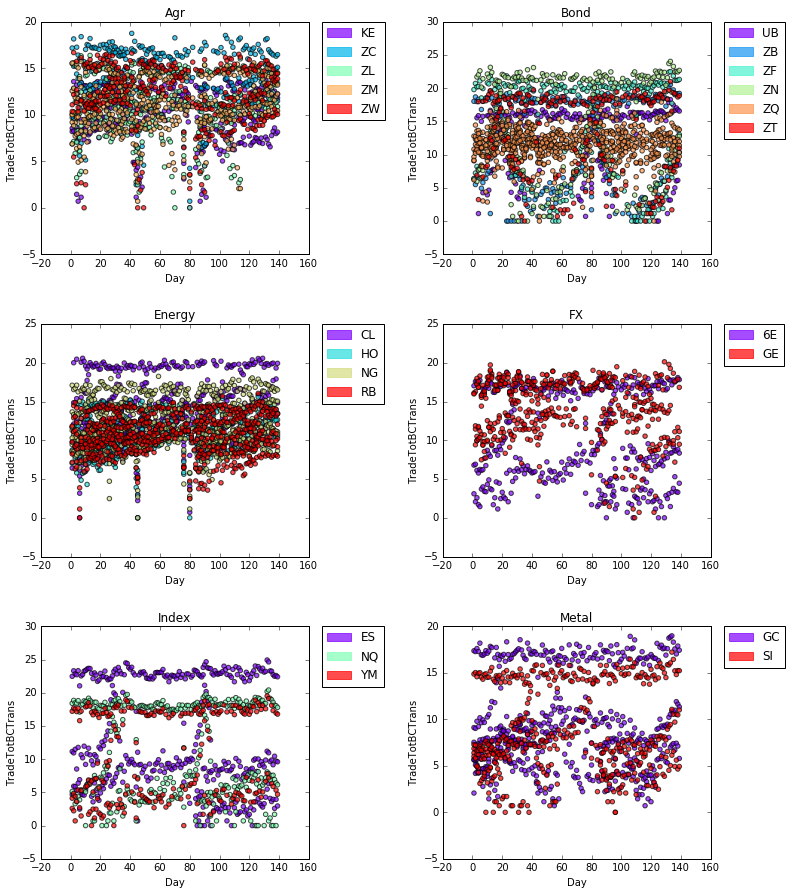
\includegraphics[width=15cm]{agr_scatter_transMat.png} %change dim to 15 by 17 in python code
		\caption{Plot of trade volume as days pass for instrument types}
		\label{fig:3}
	\end{center}
\end{figure}

\noindent metal are not. Therefore we expect higher error in the spline model of the latter compared to the former group of instruments. The trend in daily trade volume as time passed was also explored for each instrument market in Figure 4.  These points were then color-coded to understand which instruments comprised the various clusters. It is clear that low volumes of trading occur for metal and agriculture markets compared with bond and index markets which appear to be more liquid. 

\begin{figure}[H]
	\begin{center}	
		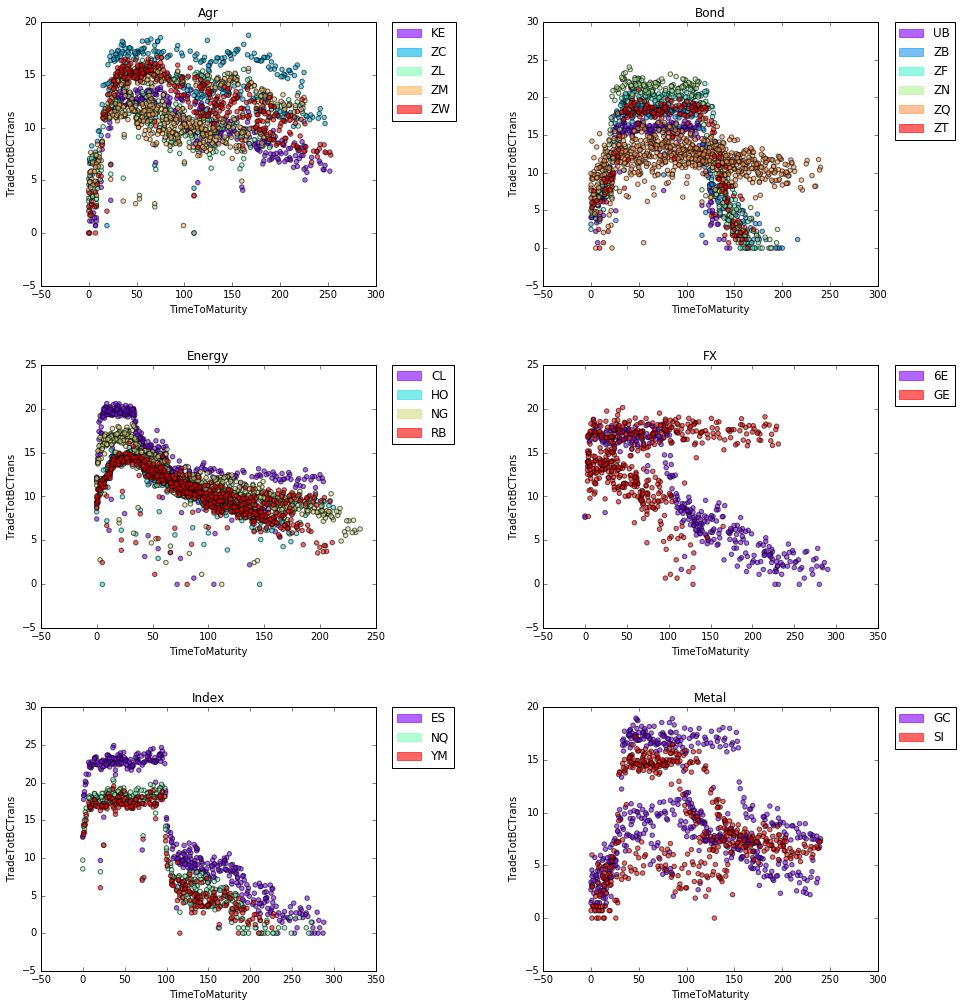
\includegraphics[width=15cm]{types_time_to_mat.png}
		\caption{Plot of trade volume as time to maturity gets further for instrument types}
		\label{fig:4}
	\end{center}
\end{figure}

Finally, in Figure 5, the trend in daily trade volume as time to maturity increased was visualized for each market. Like the histograms, agriculture, bond, and energy plots follow the general trend of low trade volume far from the maturity and close to maturity, but foreign exchange, index, and metal do not. There is some clustering in the index and metal plots as well which seems in line with the trimodal and bimodal histograms respectively in 
Figure 3. This clustering is also consistent with plots in Figure 4.

%Regression
The above described exploratory analysis deemed spline regression reasonable for trade volume prediction. Thus, both one linear model and multiple linear models paradigms were considered, two versions for each, making four models in total as shown in Table 1. All models under consideration were linear. One model paradigm employed a single model for all markets, whereas in the multiple models paradigm each market had its own model. Spline variables are denoted by ``s". The models were fit on data from May 2, 2016 to August 2, 2016 and tested or forecasted on data from August 2, 2016 through November 18, 2016. The mean absolute deviation (MAD) was then calculated for each model to compare the errors of forecasted volumes in a robust manner. MAD is defined as: $\displaystyle \sum_{i=1}^{N} \frac{|\hat{Y_i}-Y_i|}{N}$. The models were penalized with an integrated square second derivative cubic spline. This amounted to a natural spline and so generalized cross validation was employed to find an optimal smoothing parameter. The knots were placed at fixed intervals.
%smooth.terms {mgcv}
%smooth.construct.cr.smooth.spec {mgcv}	

\begin{table}[H]
	\caption{Predictors used in models}
	\begin{center}
		\begin{tabular}{ |c|c|c|c| } 
		\hline
		\multicolumn{2}{| c |}{One Linear Model}
		&
		\multicolumn{2}{| c |}{Multiple Linear Models}\\
		\hline
		\hline
		Model 1' & Model 1 & Model 2' & Model 2\\
		\hline
		 s(TimeToMaturity) & s(TimeToMaturity) & s(TimeToMaturity) & s(TimeToMaturity) \\ 
		s(DayofMonth) & s(DayofMonth) & s(DayofMonth) & s(DayofMonth) \\ 
		Market & Market & DayOfTheWeek & DayOfTheWeek \\ 
		DayOfTheWeek & DayOfTheWeek &  & Instrument \\
		           & Instrument &  & \\
		\hline
		\end{tabular}
	\end{center}
	\label{tab:dum1}
\end{table}

An additional goal of this study was to understand the relationship between price volatility and trade volume. To this end, hourly aggregation similar to that which was done for trade volume was done for price volatility. Volatility was measured using standard deviation. Data was filtered for products with more 30 or more days of data. Next each product's daily price was plotted against daily trade volume for the full period over which the data was collected; that is from May to November. Hourly price volatility was plotted against its hourly trade volume was also plotted. Given past research, we expect a positive correlation between price and volume. Consistency of the correlation between price and volume over the days was of interest as well. This was investigated for each product by plotting daily correlations between hourly price volatility and hourly trade volume. 

Observations with trade counts within the 60th to 90th percentiles were used to identify periods of normal trade volumes. In other words, to avoid the nascent and near maturity periods of low trading which would confound results, only records rep-

\begin{figure}[H]
	\begin{center}
		\begin{tabular}{cc}
			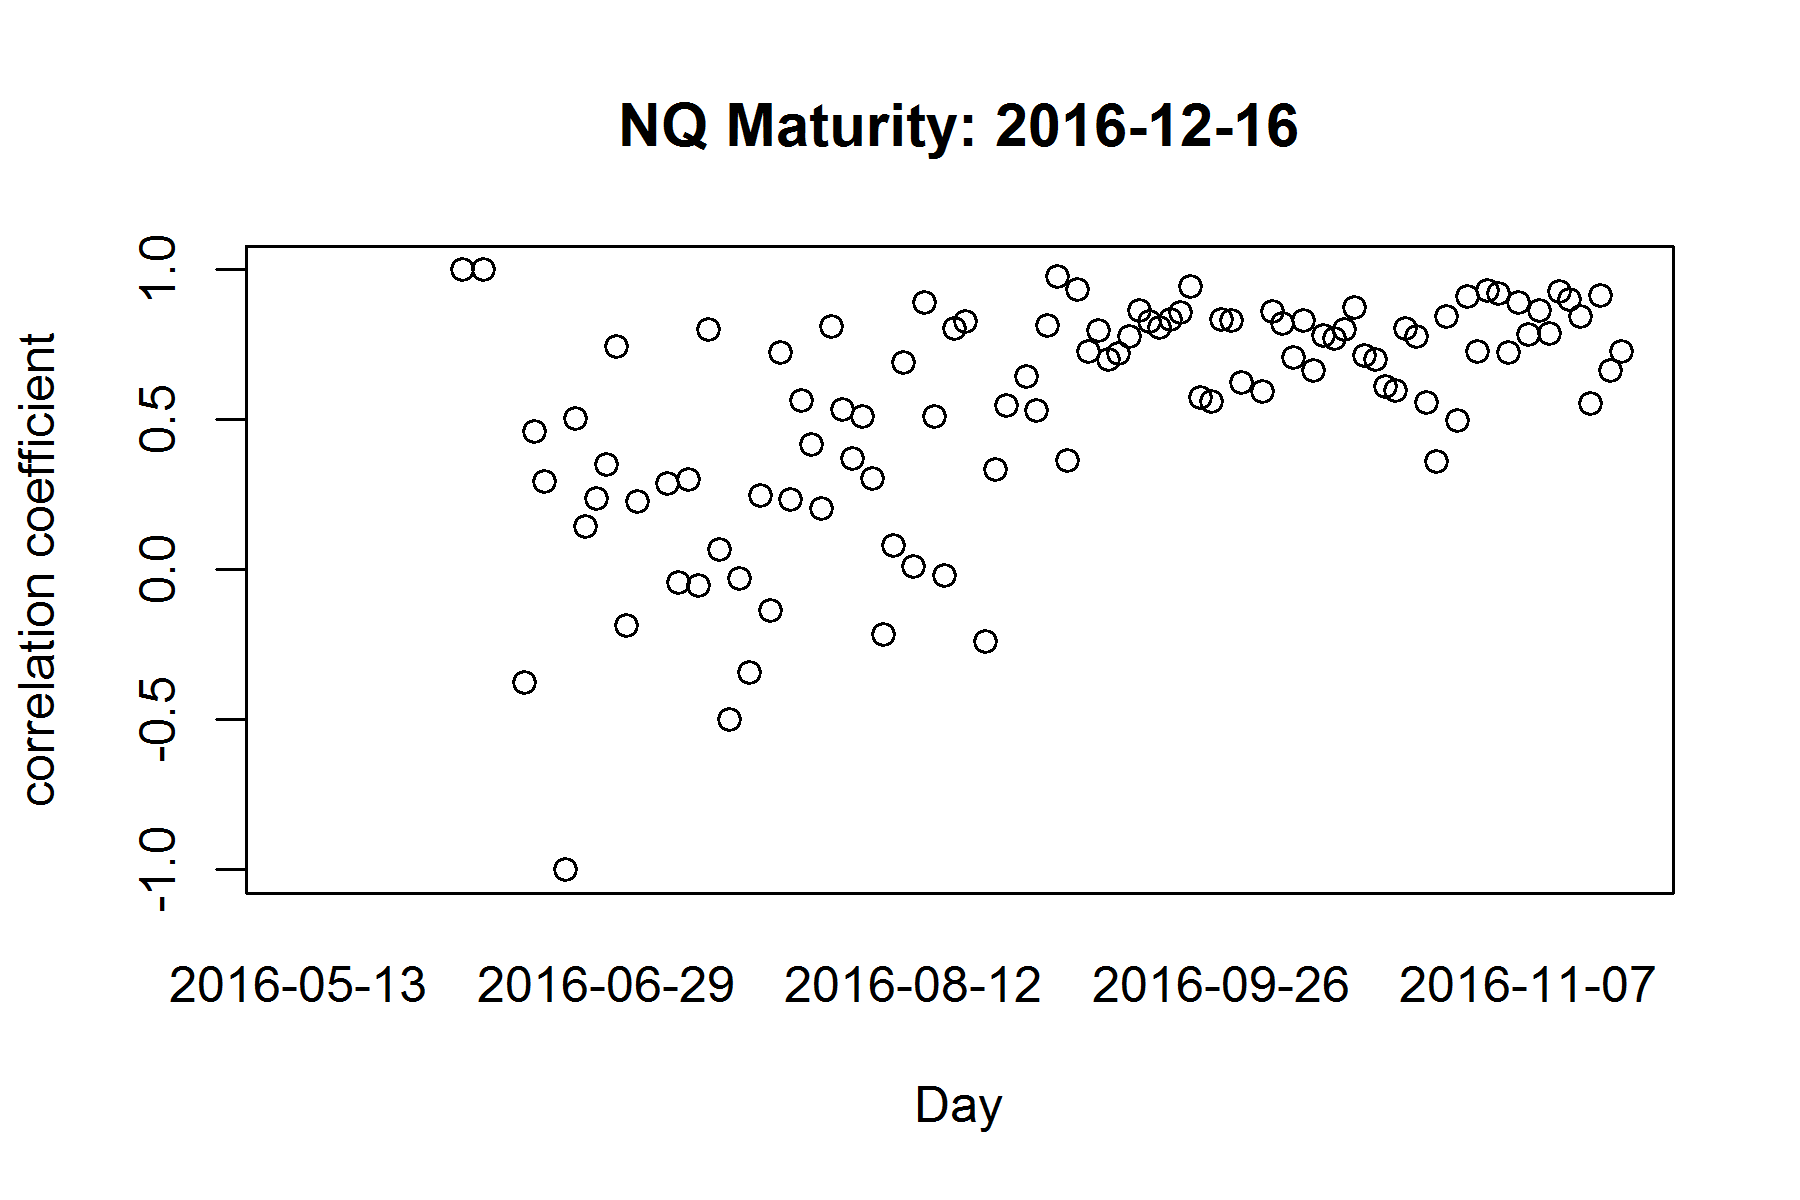
\includegraphics[width=10cm]{NQcor_plot.png} \\ 
			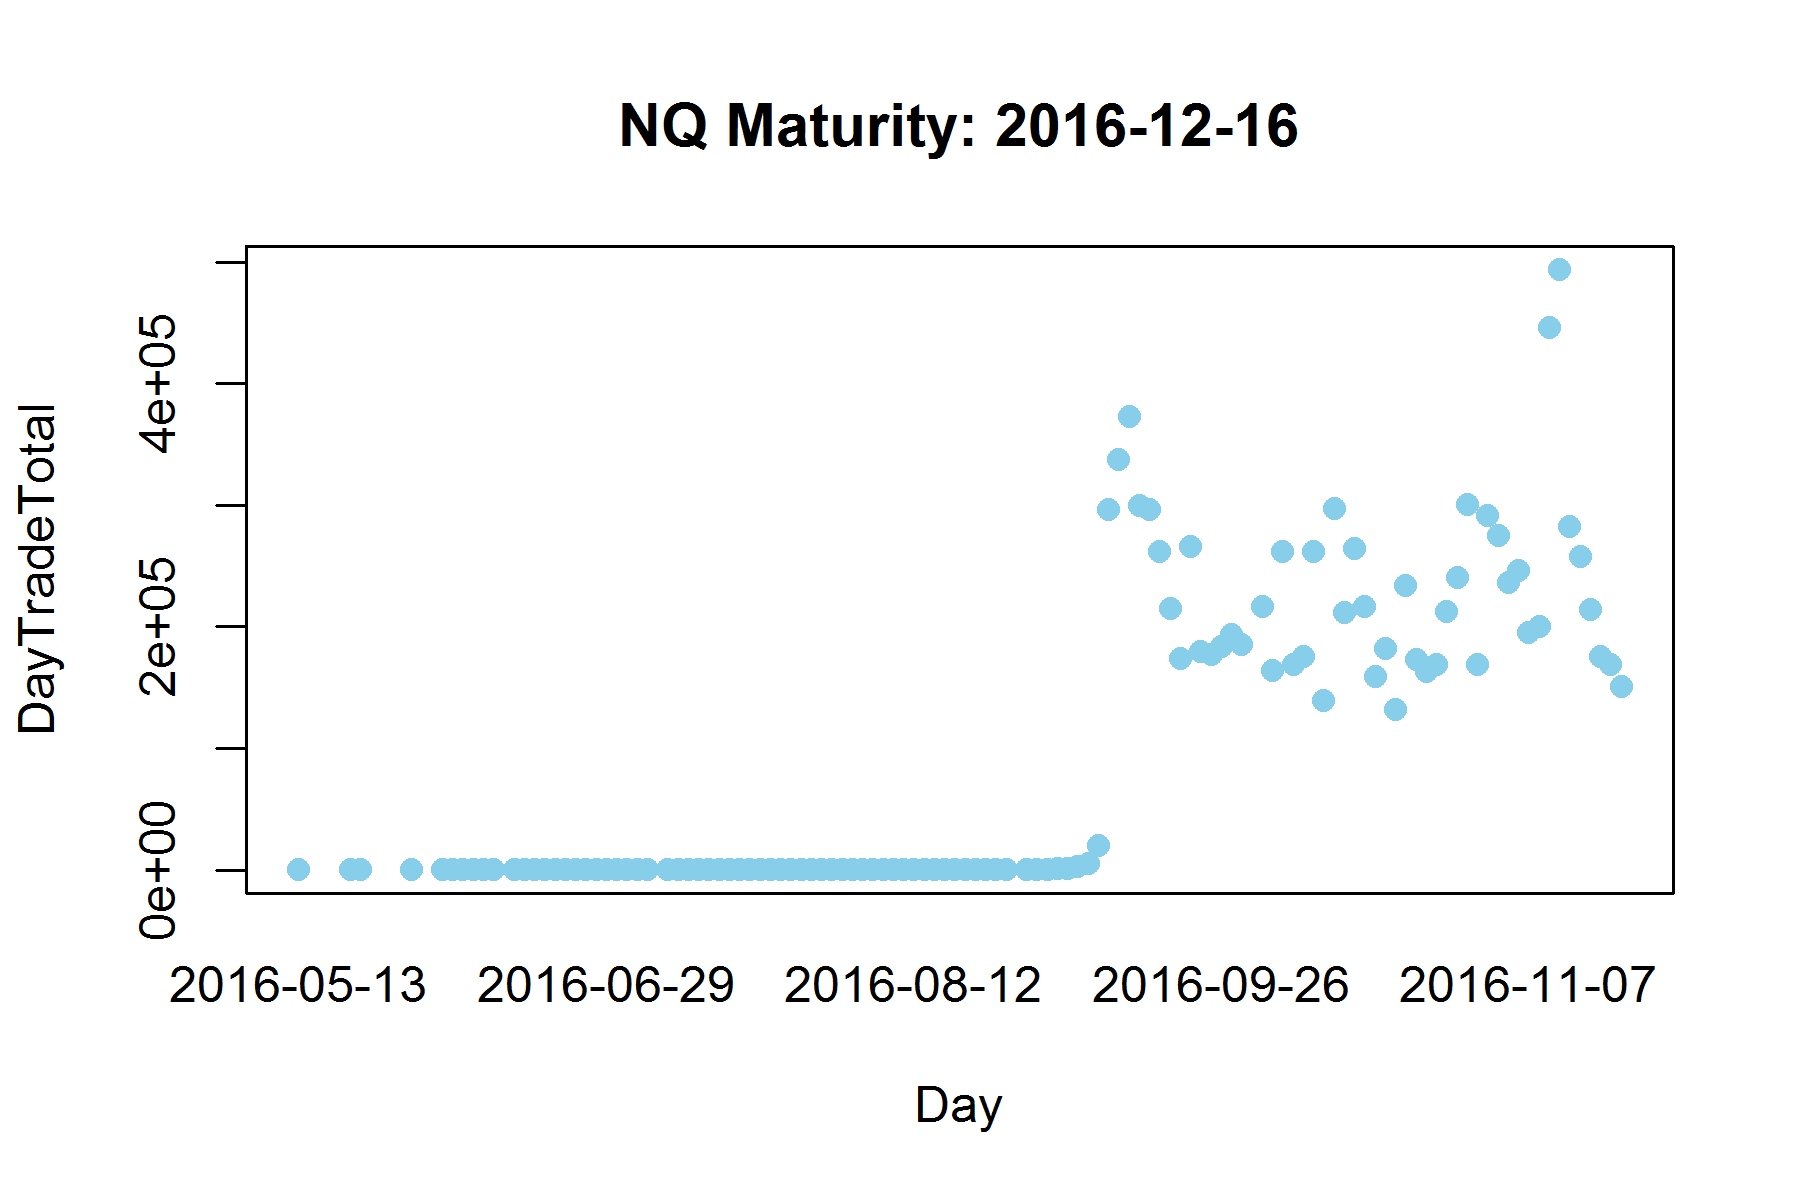
\includegraphics[width=10cm]{NQtradevolume.png}	\\ 
		\end{tabular}
	\end{center}
	\caption{Correlation (top) and trade volume (bottom) for NQ maturing 2016-12-16}
	\label{fig:NQ}
\end{figure}

\noindent resenting a product's active period were selected. The E-Mini Nasdaq 100 (NQ) with maturity 2016-12-16 is a product whose nascent period is captured in the time frame data was recorded, as demonstrated in Figure 6. From the top of Figure 6, it is clear that the correlation between price volatility and trade volume stabilizes around 2016-09-15. Looking at the bottom of Figure 6, 2016-09-15 is also the time that the daily trade volume makes a sharp increase from zero to around 100,000.  

\begin{figure}[H]
	\begin{center}
		\begin{tabular}{cc}
			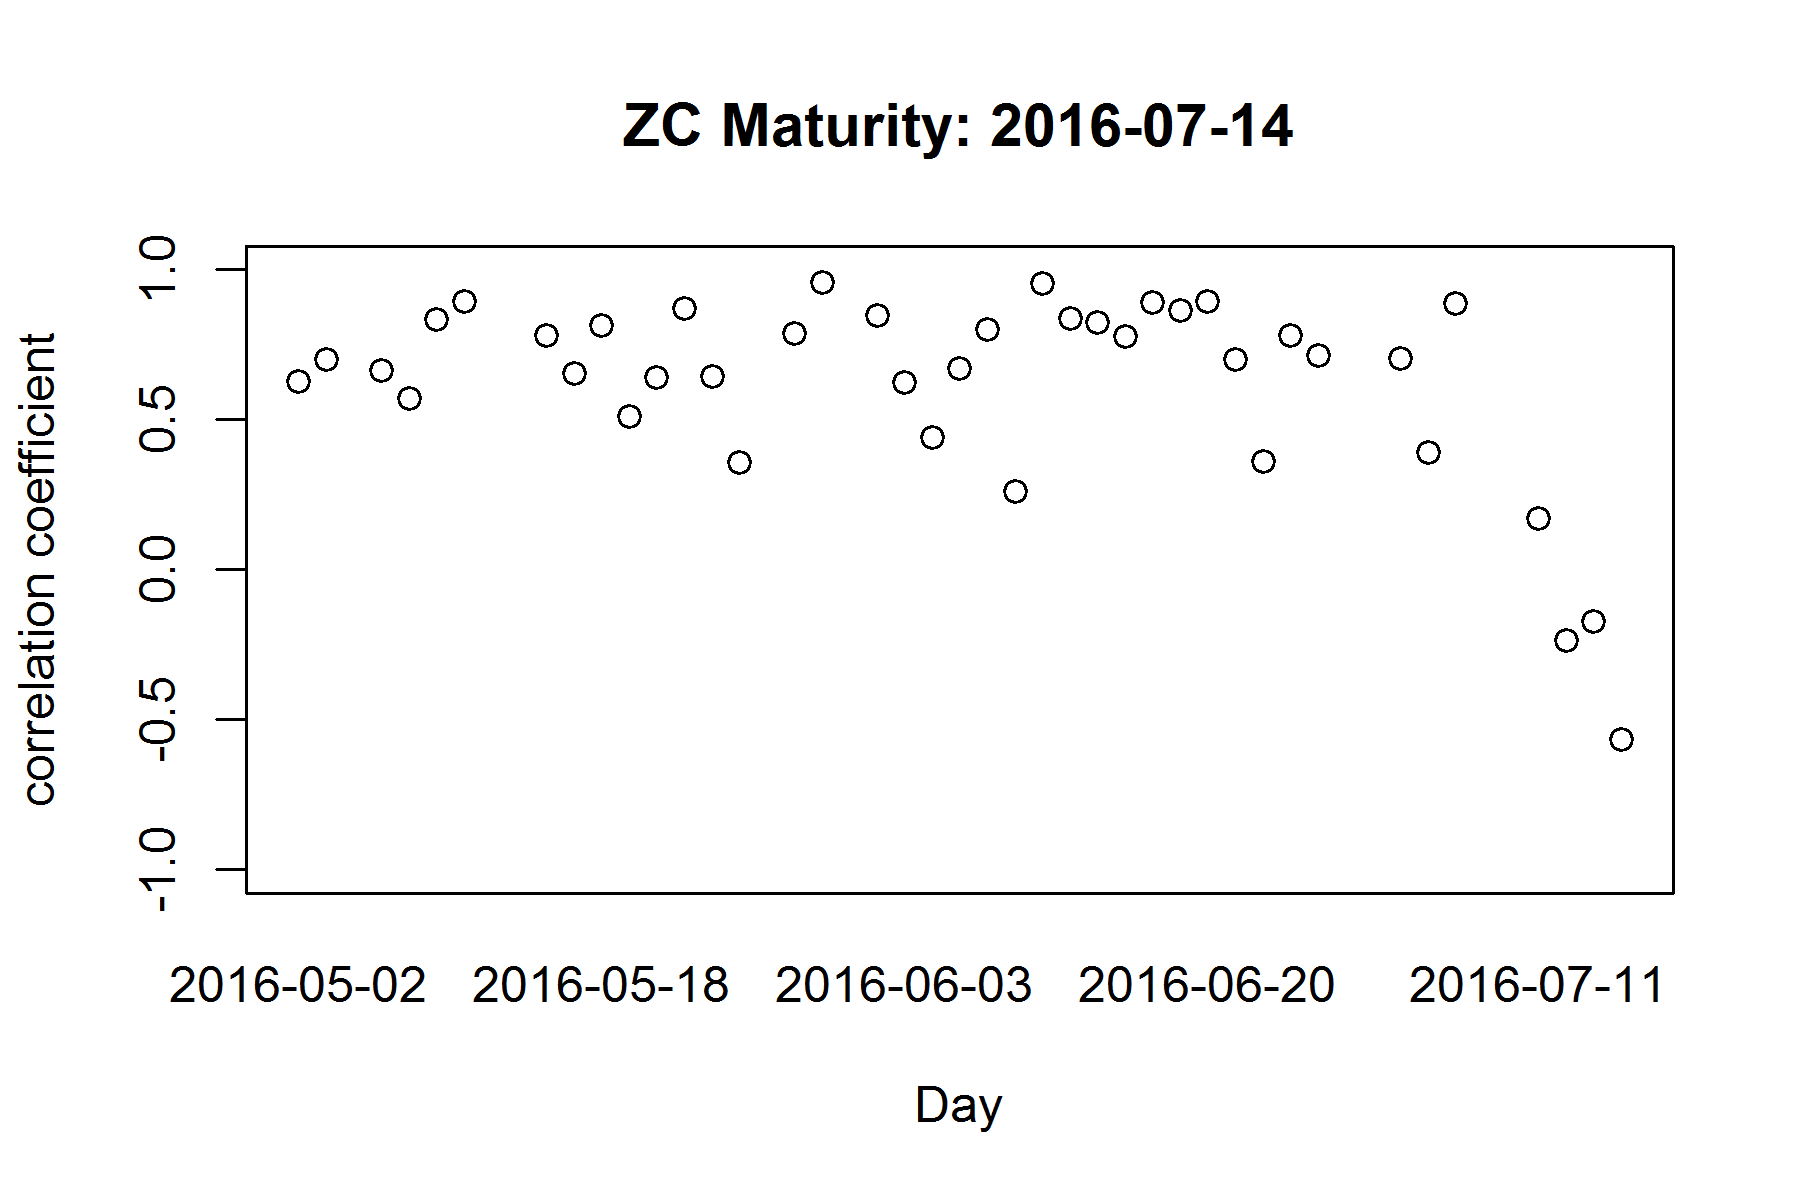
\includegraphics[width=10cm]{ZCcor_plot.png} \\ 
			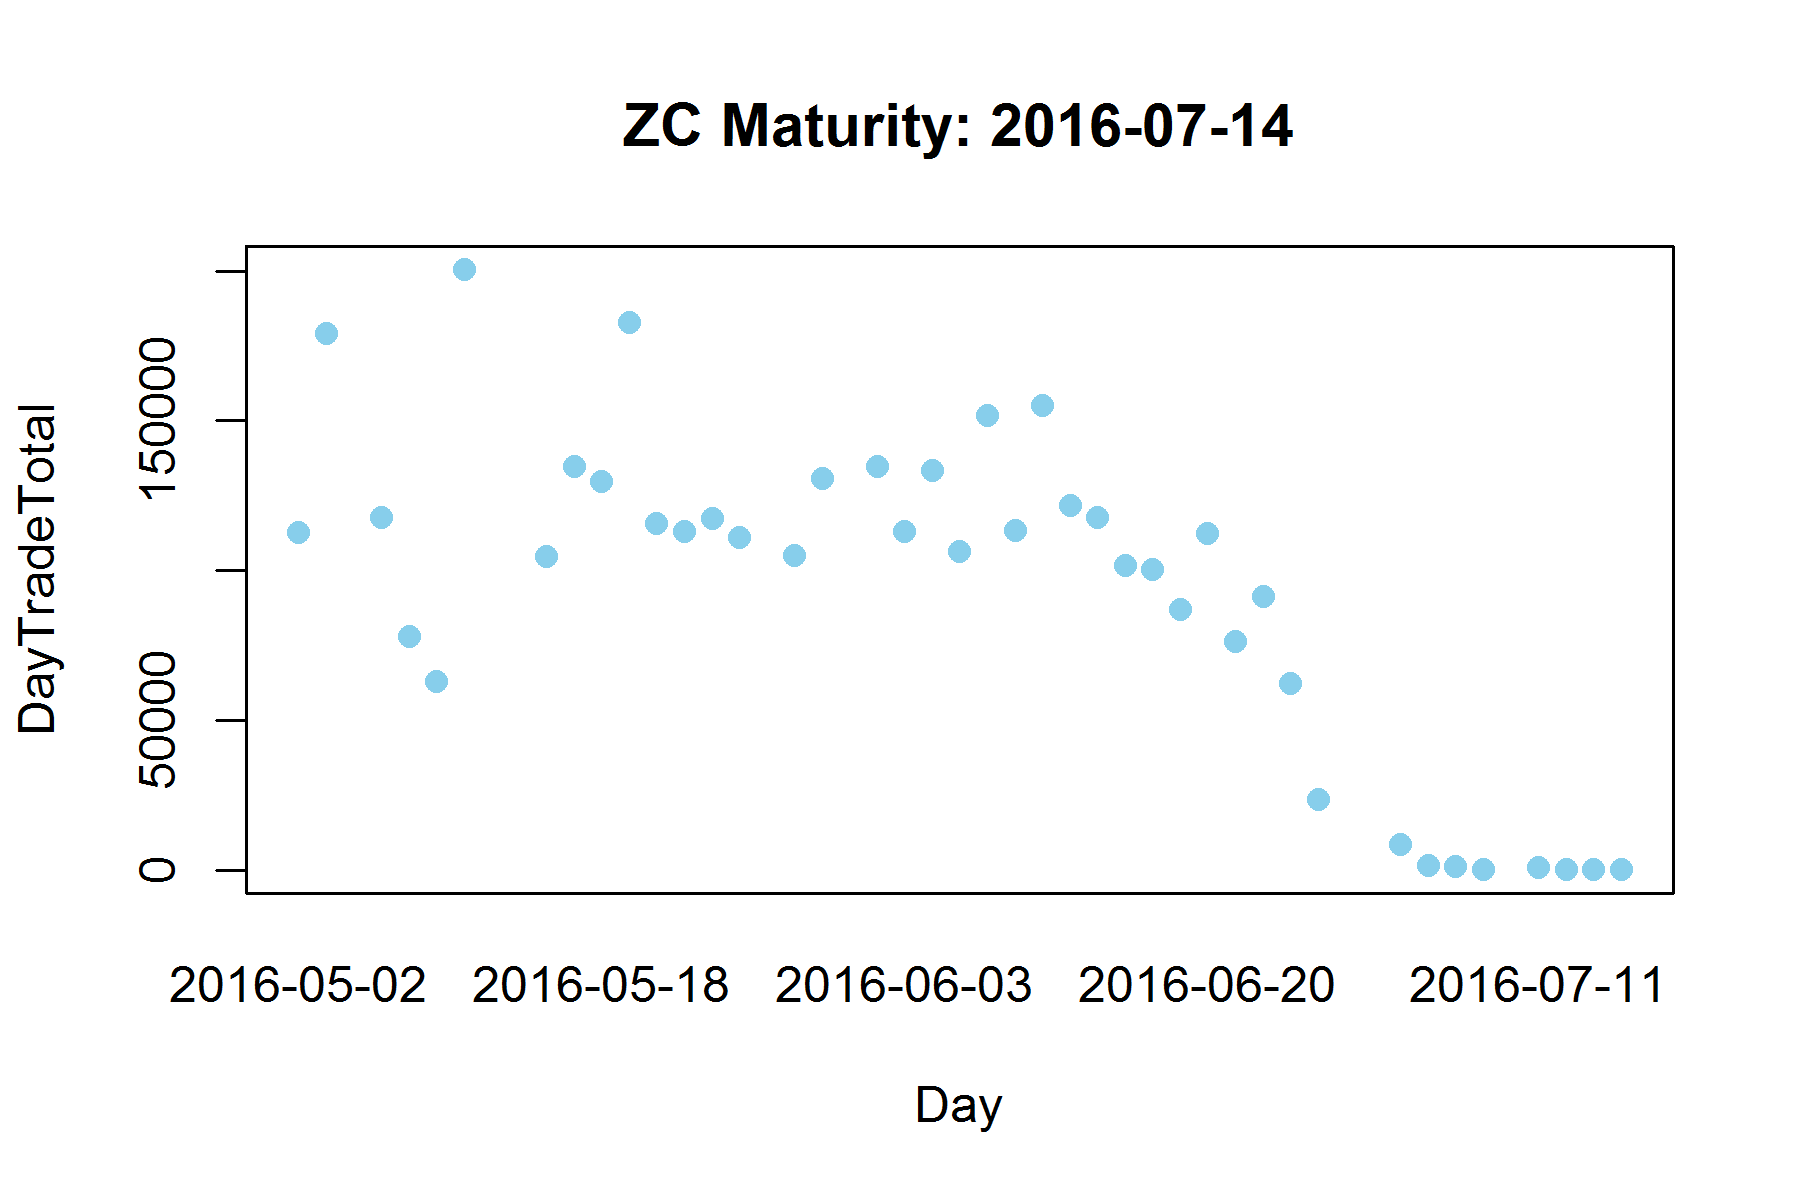
\includegraphics[width=10cm]{ZCtradevolume.png}	\\ 
		\end{tabular}
	\end{center}
	\caption{Correlation (top) and trade volume (bottom) for ZC maturing 2016-07-14}
	\label{fig:ZC}
\end{figure}

Corn (ZC) with maturity 2016-07-14 is a product whose near maturity period is captured in the time frame data was recorded, as demonstrated in Figure 7. Like NQ, the top of Figure 7 shows that the correlation for ZC is constant until around 2016-07-01. Looking at the bottom of Figure 7, 2016-07-01 is also the time that the daily trade volume makes a sharp decrease from 65,000 to zero.

After records in a product's active period were selected, linear regression was  done on the correlation coefficient between the price volatility and trade volume to test whether the best fit line was constant or flat. A flat regression line would mean that the expected correlation between price volatility did not change with time.

\section*{Results} 
\addcontentsline{toc}{section}{Results}

%for trade quantity regression
The best linear regression model is Model 2 based on Table 2 since Model 2 has the lowest MAD across markets. Thus the multiple models paradigm is better than the one model paradigm. 

\begin{table}[H]
	\centering
	\caption{Linear models comparison at market level}
	\label{Table 2}
	\begin{tabular}{|c|c|c|c|c|c|c|c|}
		\hline
		\multirow{2}{*}{}                & Market      & Metal & Bond   & Agr    & Energy & Index & FX     \\ \cline{2-8} 
		& Median       & 7.98  & 12.512 & 11.579 & 11.751 & 9.705 & 12.478 \\ \hline
		\multirow{2}{*}{One Model}       & Model 1' MAD & 3.537 & 3.742  & 2.261  & 1.958  & 5.103 & 4.223  \\ \cline{2-8} 
		& Model 1 MAD  & 3.603 & 3.615  & 1.809  & 1.818  & 5.455 & 4.08   \\ \hline
		\multirow{2}{*}{Multiple Models} & Model 2' MAD & 3.966 & 4.463  & 3.966  & 4.463  & 3.966 & 4.463  \\ \cline{2-8} 
		& Model 2 MAD  & 3.023 & 3.174  & 2.103  & 1.327  & 1.591 & 3.753  \\ \hline
	\end{tabular}
\end{table}

Referring to Table 3, at the instrument level MAD is lower for Model 2 than Model 2' for the most part. Given its superiority at the market level, it is not surprising that model 2 is also superior at the instrument level. 

Figure 8 shows that the time to maturity influences trade volume more significantly than day of the month since all the day of the month cubic spline curves hover around zero.

\begin{table}[H]
	\centering
	\caption{Multiple linear models comparison at instrument level}
	\label{Table 3}
	\begin{tabular}{|c|c|c|c|}
		\hline
		\multicolumn{4}{|c|}{Multiple Linear Models}     \\ \hline
		Instrument & Median & Model 2' MAD & Model 2 MAD \\ \hline
		GC         & 8.1    & 3.417        & 2.914       \\ \hline
		SI         & 7.807  & 3.685        & 3.158       \\ \hline
		ZQ         & 11.944 & 2.159        & 3.066       \\ \hline
		ZT         & 16.55  & 4.229        & 2.5         \\ \hline
		ZF         & 19.266 & 5.222        & 3.095       \\ \hline
		ZB         & 12.466 & 4.665        & 3.313       \\ \hline
		UB         & 15.629 & 2.762        & 2.642       \\ \hline
		ZN         & 19.061 & 5.473        & 4.335       \\ \hline
		ZW         & 11.917 & 1.963        & 2.269       \\ \hline
		ZM         & 10.891 & 2.302        & 2.071       \\ \hline
		KE         & 10.514 & 1.76         & 2.009       \\ \hline
		ZC         & 13.935 & 3.303        & 2.202       \\ \hline
		ZL         & 11.099 & 2.139        & 2.004       \\ \hline
		CL         & 14.407 & 2.744        & 1.556       \\ \hline
		NG         & 11.549 & 1.929        & 1.26        \\ \hline
		HO         & 11.083 & 1.912        & 1.251       \\ \hline
		RB         & 10.907 & 1.497        & 1.299       \\ \hline
		NQ         & 16.341 & 4.997        & 1.607       \\ \hline
		ES         & 9.624  & 5.664        & 1.765       \\ \hline
		YM         & 9.087  & 4.271        & 1.262       \\ \hline
		GE         & 13.956 & 3.966        & 3.724       \\ \hline
		6E         & 8.244  & 4.463        & 3.78        \\ \hline
	\end{tabular}
\end{table}

\begin{figure}[H]
	\begin{center}
		\begin{tabular}{ll}
		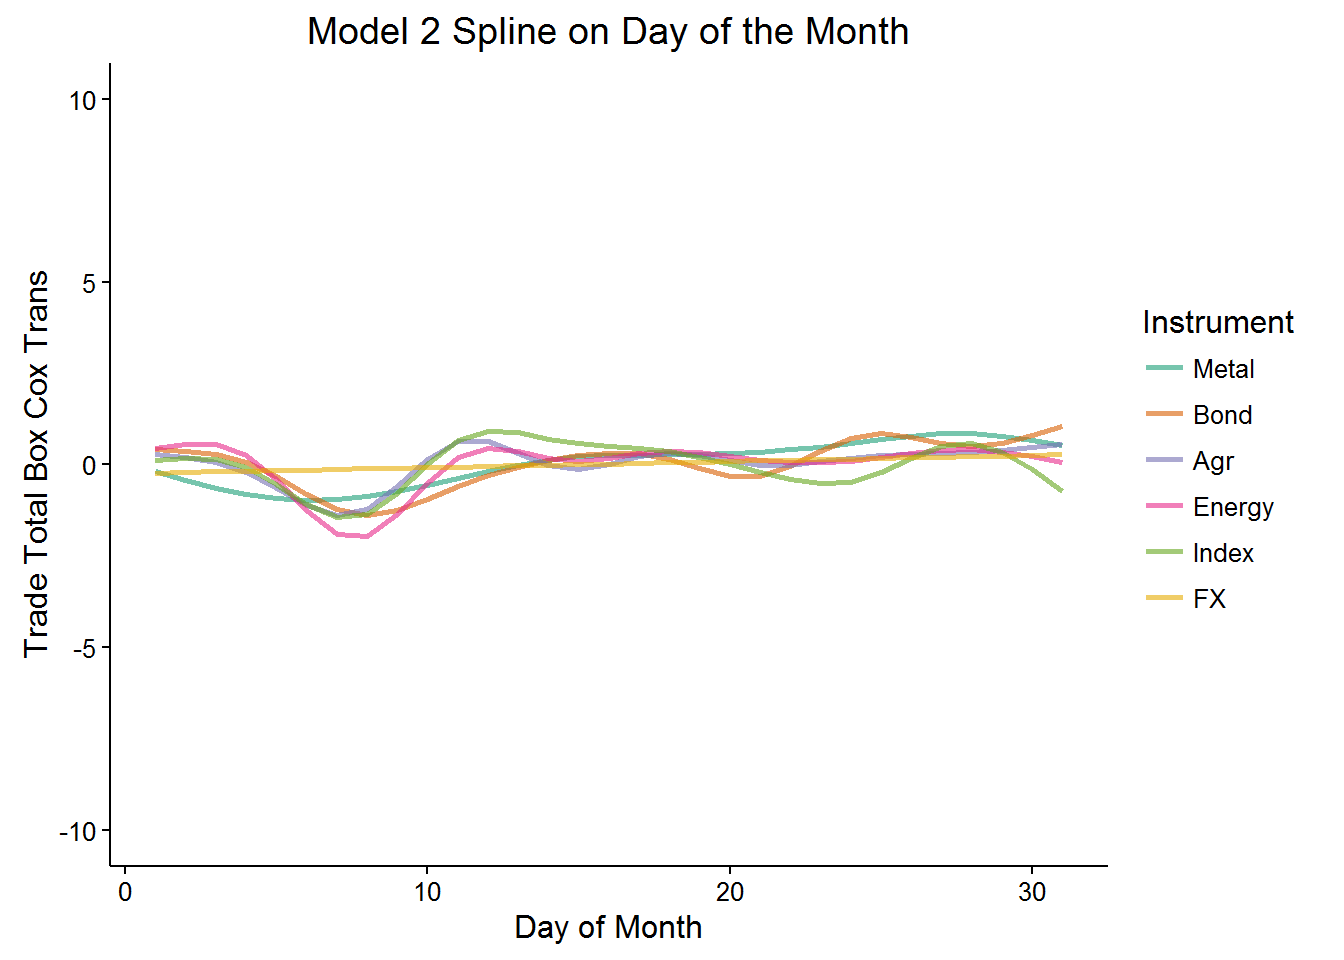
\includegraphics[width=8cm]{splineDoM.png}	&
		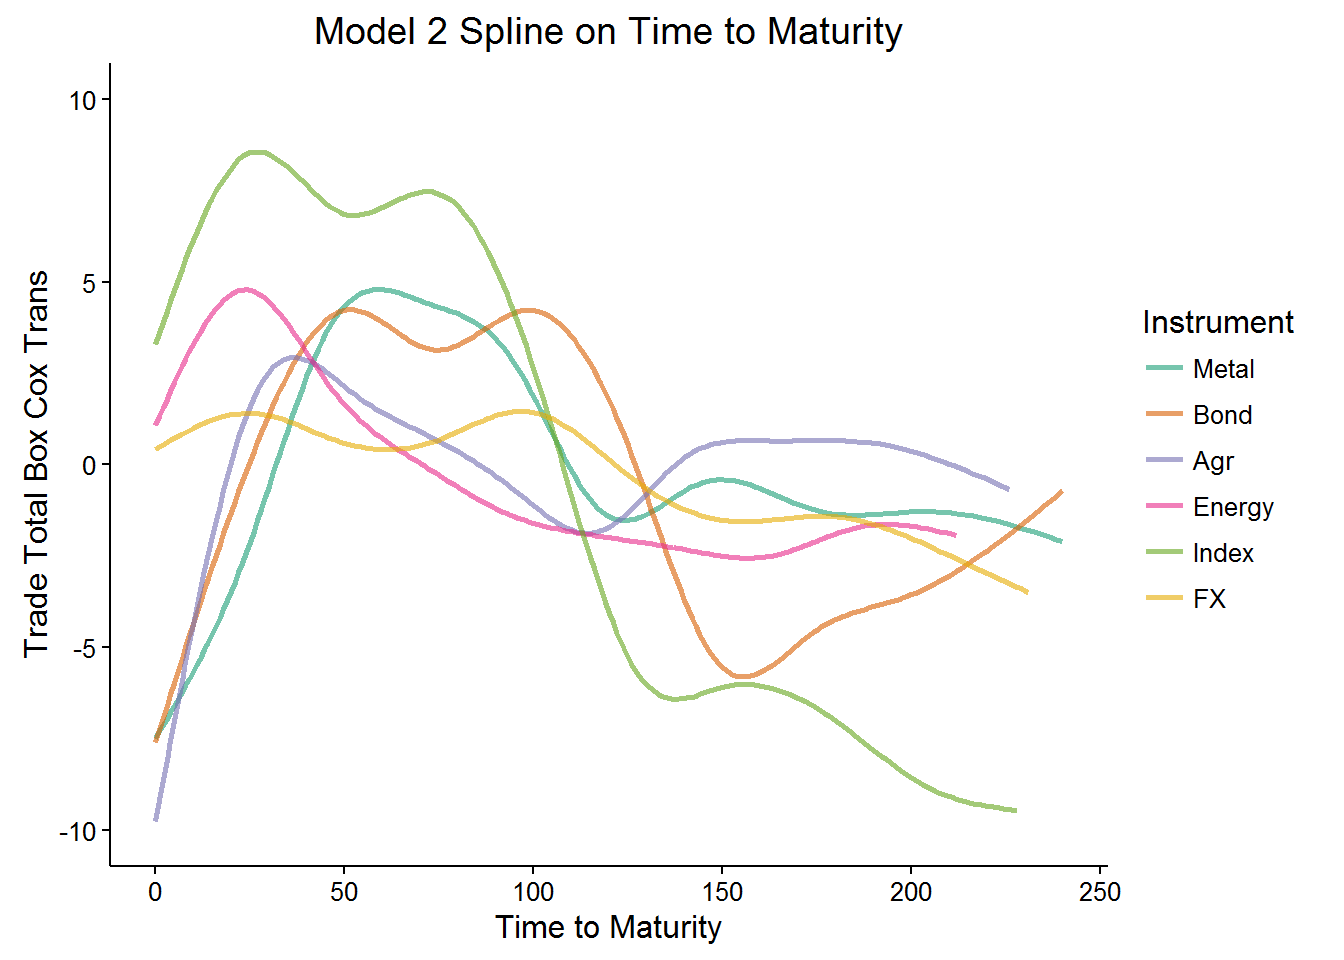
\includegraphics[width=8cm]{splineTTM.png}	\\		
		\end{tabular}
	\end{center}
	\caption{Spline curves for best model}
	\label{fig:8}
\end{figure}

%volume/vola relation
\

Figure 9 shows that p-values for testing consistency of correlations between price volatility and trade volume across products tend to be smaller than expected under the null hypothesis of constant correlations (under which the p-values should appear standard uniform). Consequently the hypothesis of constant correlations is legitimately rejected in some cases.
\begin{figure}[H]
	\begin{center}
		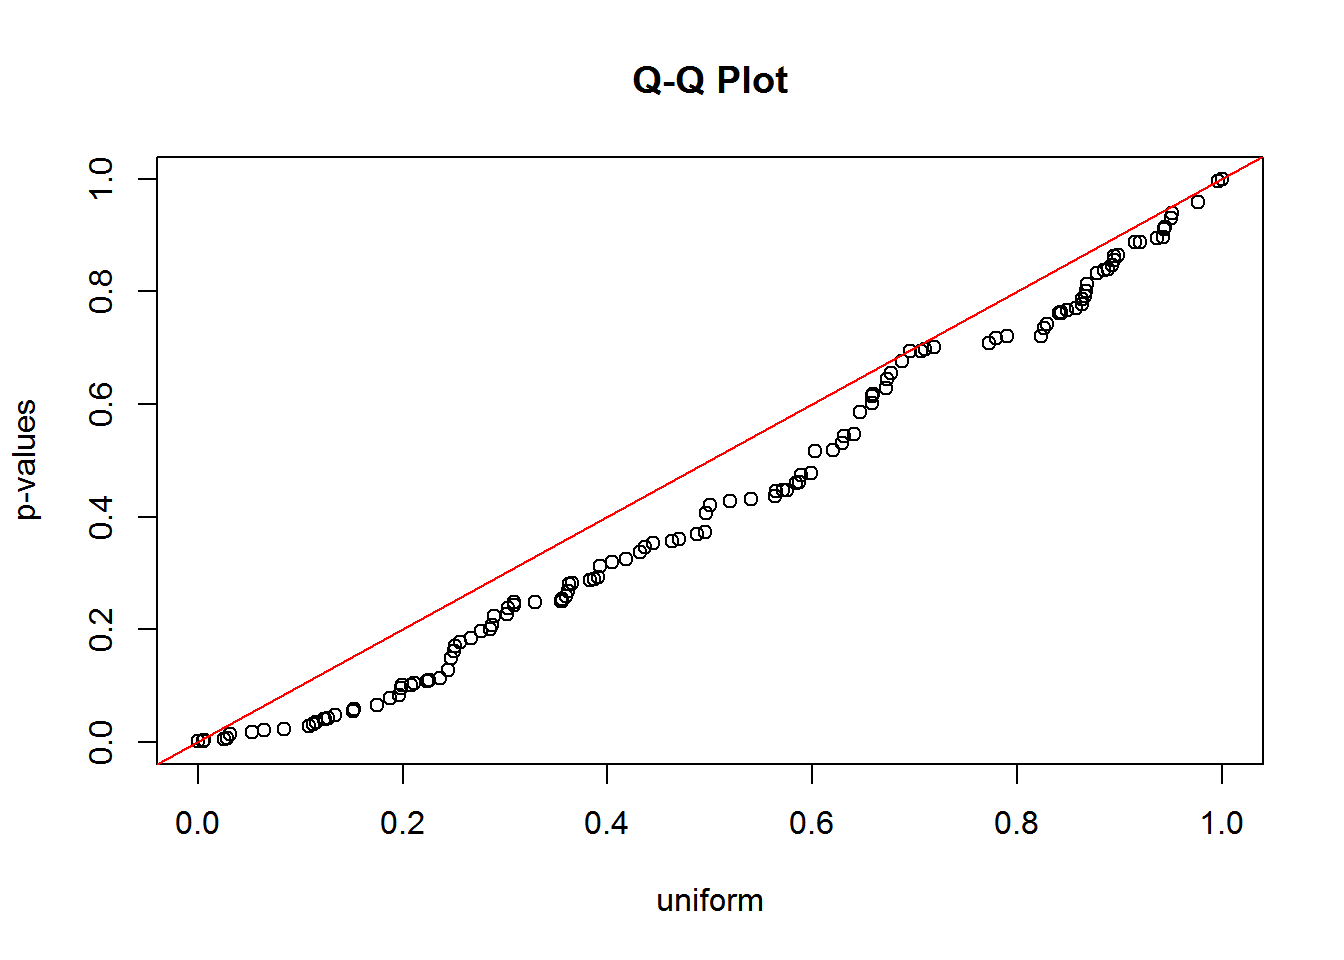
\includegraphics[width=9cm]{unifQQ2.png}
		 \vspace{-1em}	
		\caption{Uniform Q-Q plot}
		 \vspace{-1em} %reduces white space below figure
		\label{fig:9}
	\end{center}
\end{figure} 

Table 4 shows the five products, using the Benjamini-Hochberg(B-H) procedure to control false discovery rate(FDR), that were deemed as not having constant correlation, meaning the null hypothesis $\beta_1=0$ was rejected.
%http://www.tablesgenerator.com/
\begin{table}[H]
	\centering
	\caption{Significant p-values at FDR=.2}
	\label{Table 4}
	\begin{tabular}{|c|c|}
		\hline
		Product          & P-value \\ \hline
		ZQ 2016-08-31    & 0.00132        \\ \hline
		YM 2017-03-17    & 0.00222      \\ \hline
		HO 2016-11-30    & 0.00281      \\ \hline
		ZF 2016-12-30    & 0.00449      \\ \hline
		RB 2016-07-29    & 0.00693     \\ \hline
	\end{tabular}
\end{table}

The correlation plots for these five products are shown in Figure 10  with lines of best fit in red.

Figures 11 to 17 show trends in price volatility versus trade volume plots daily and hourly for the entire data collection period.
\begin{figure}[H]
	\begin{center}
		\begin{tabular}{ll}
			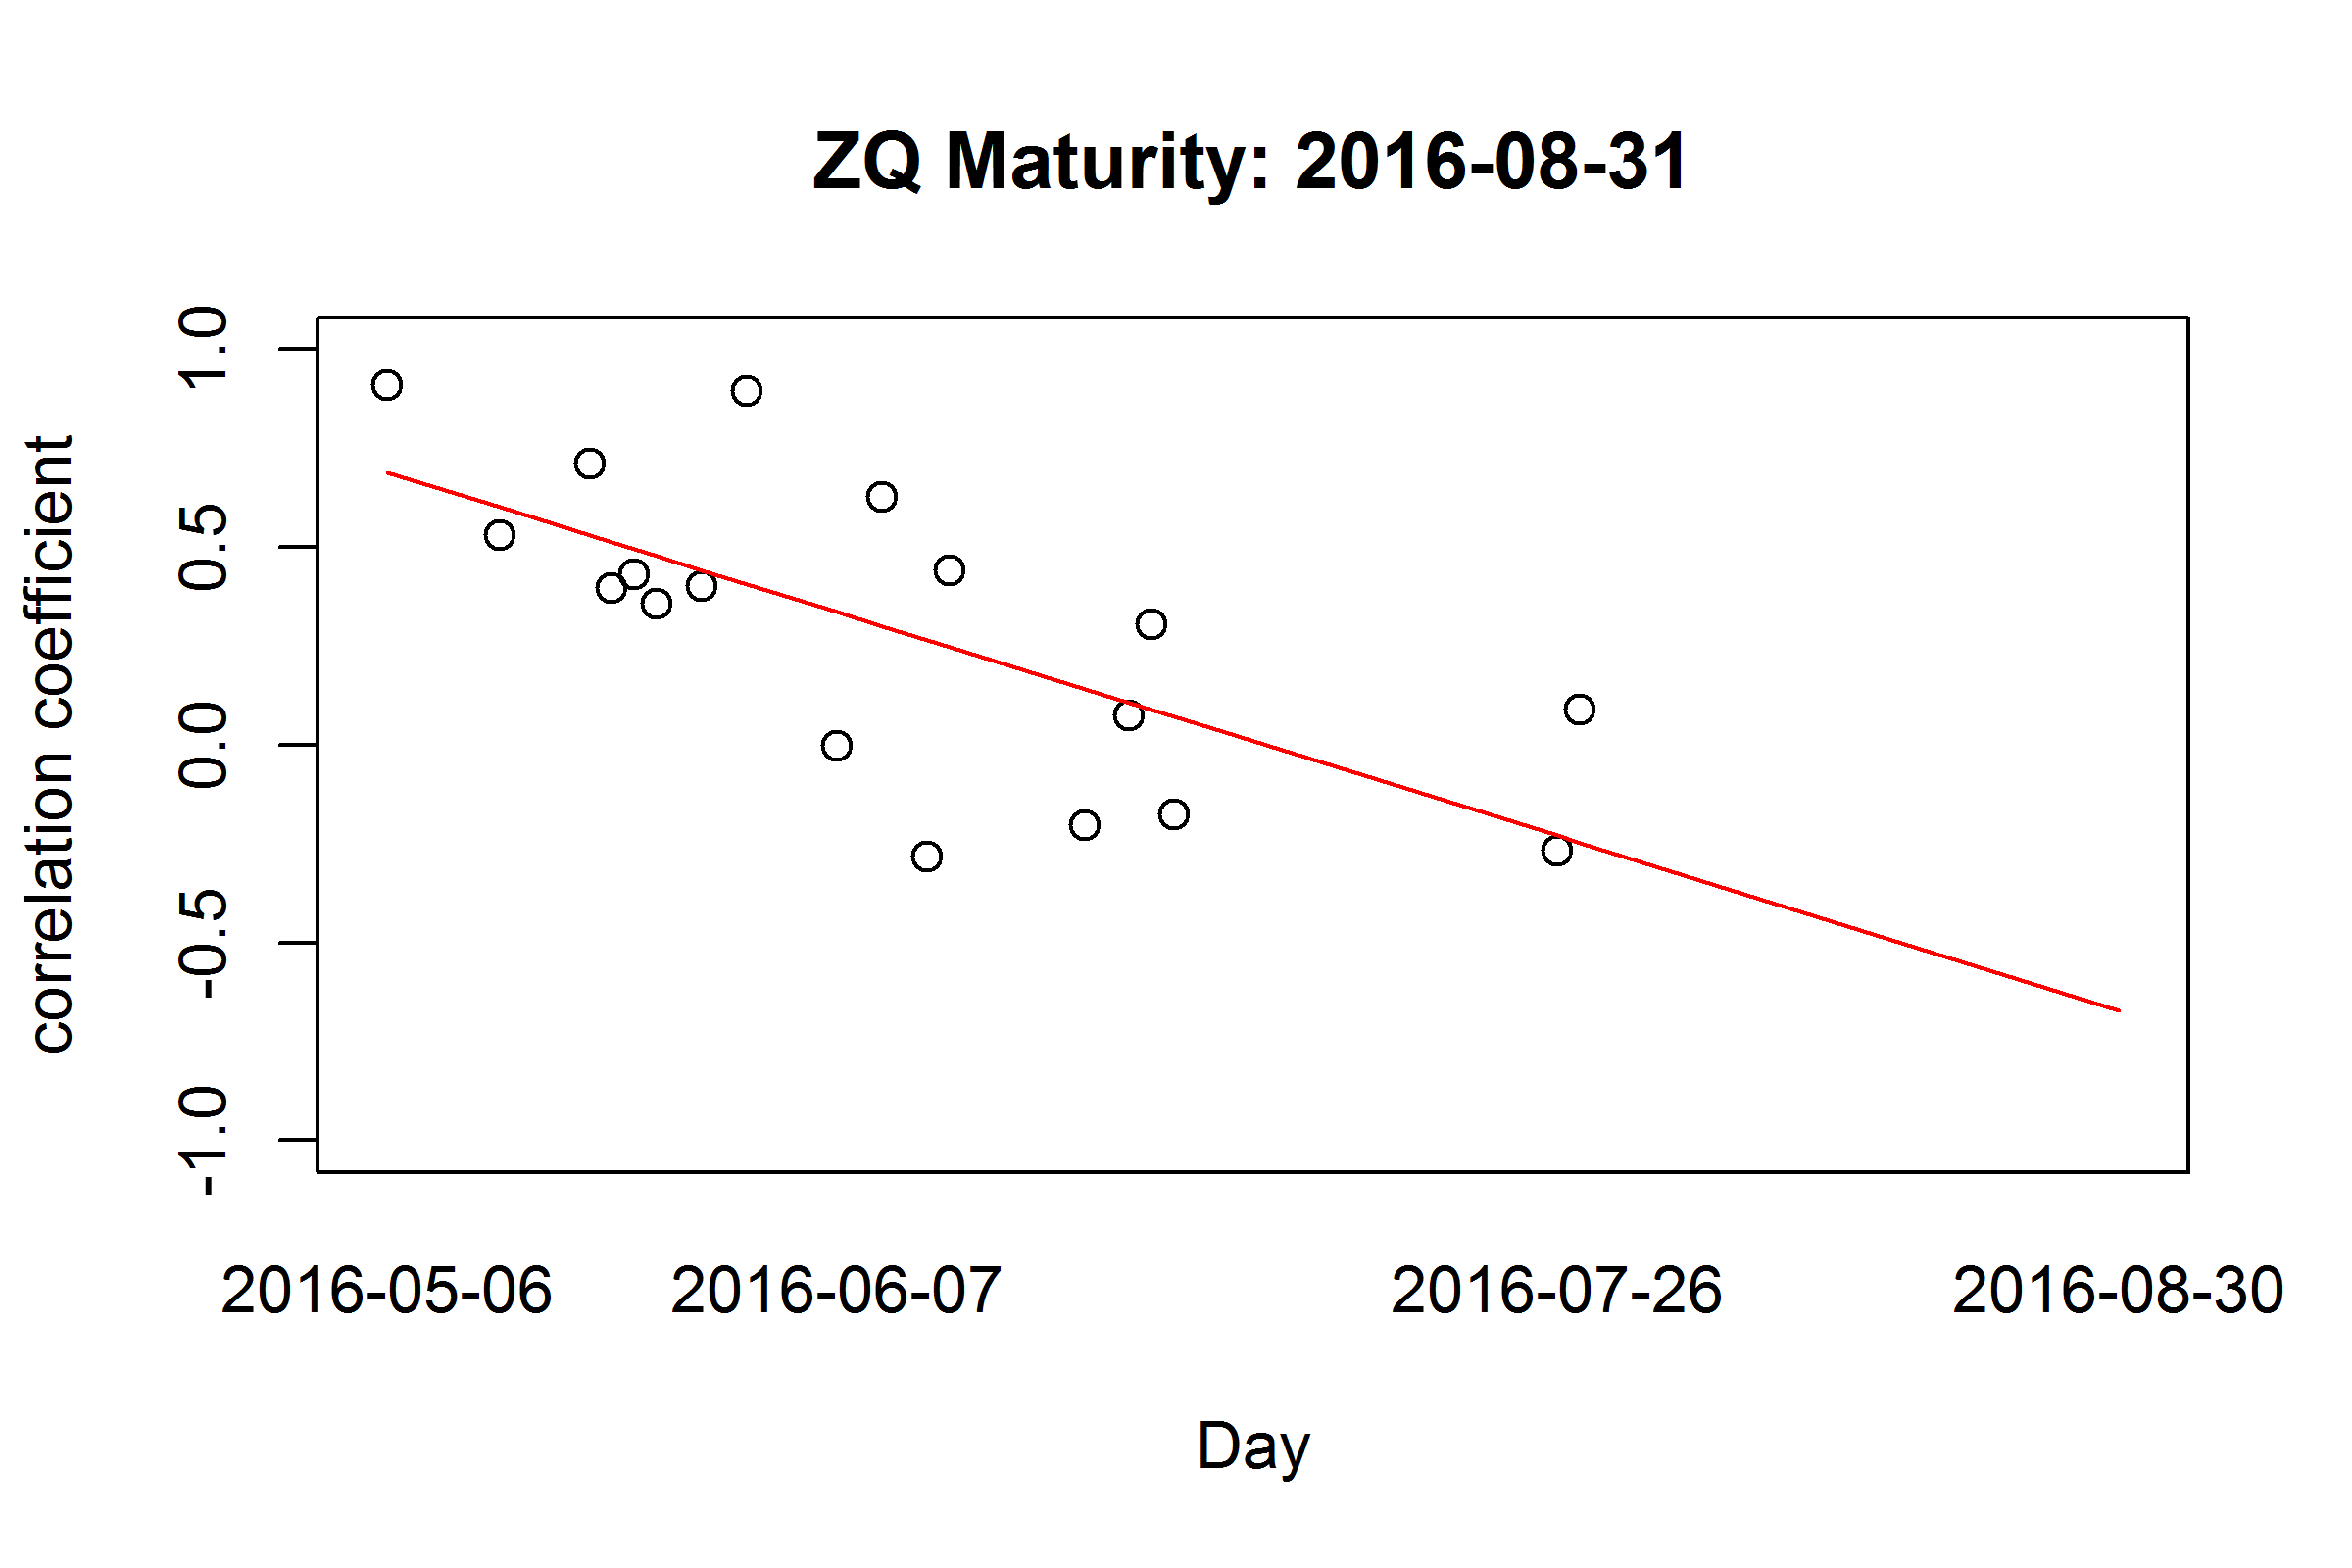
\includegraphics[width=8cm]{Coeff_fitZQ2016-08-31.png} &
			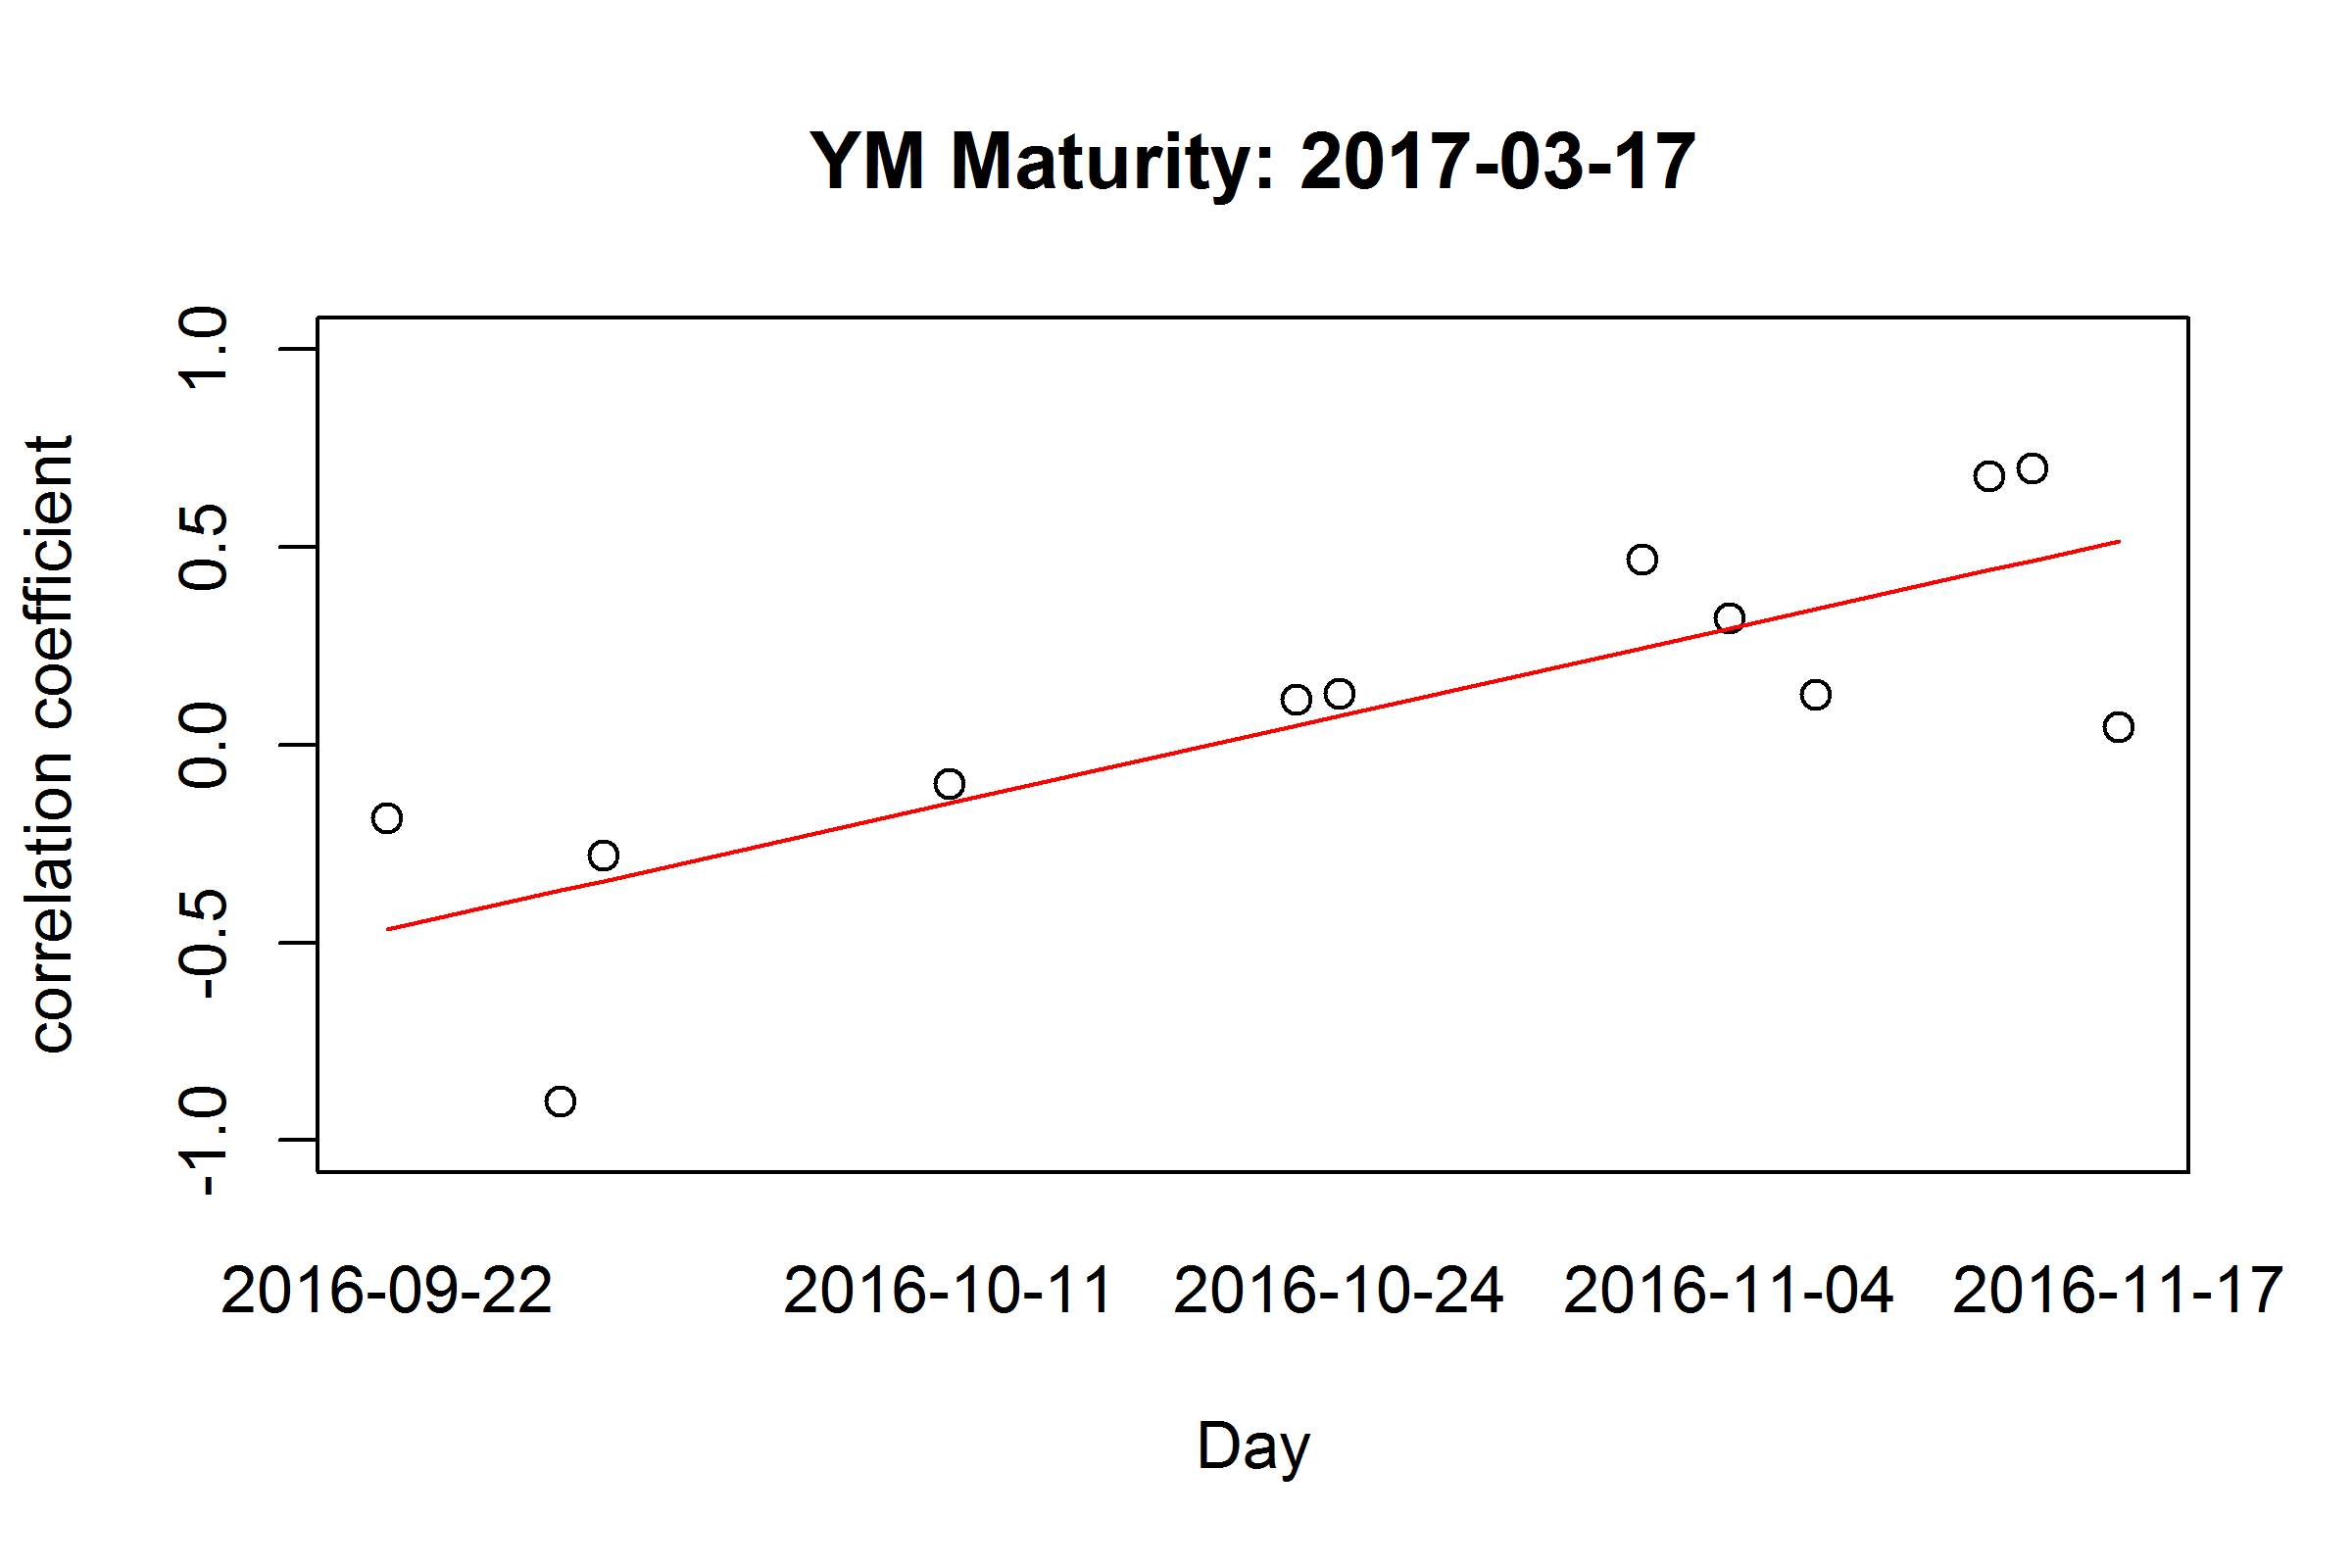
\includegraphics[width=8cm]{Coeff_fitYM2017-03-17.png}\\ 
			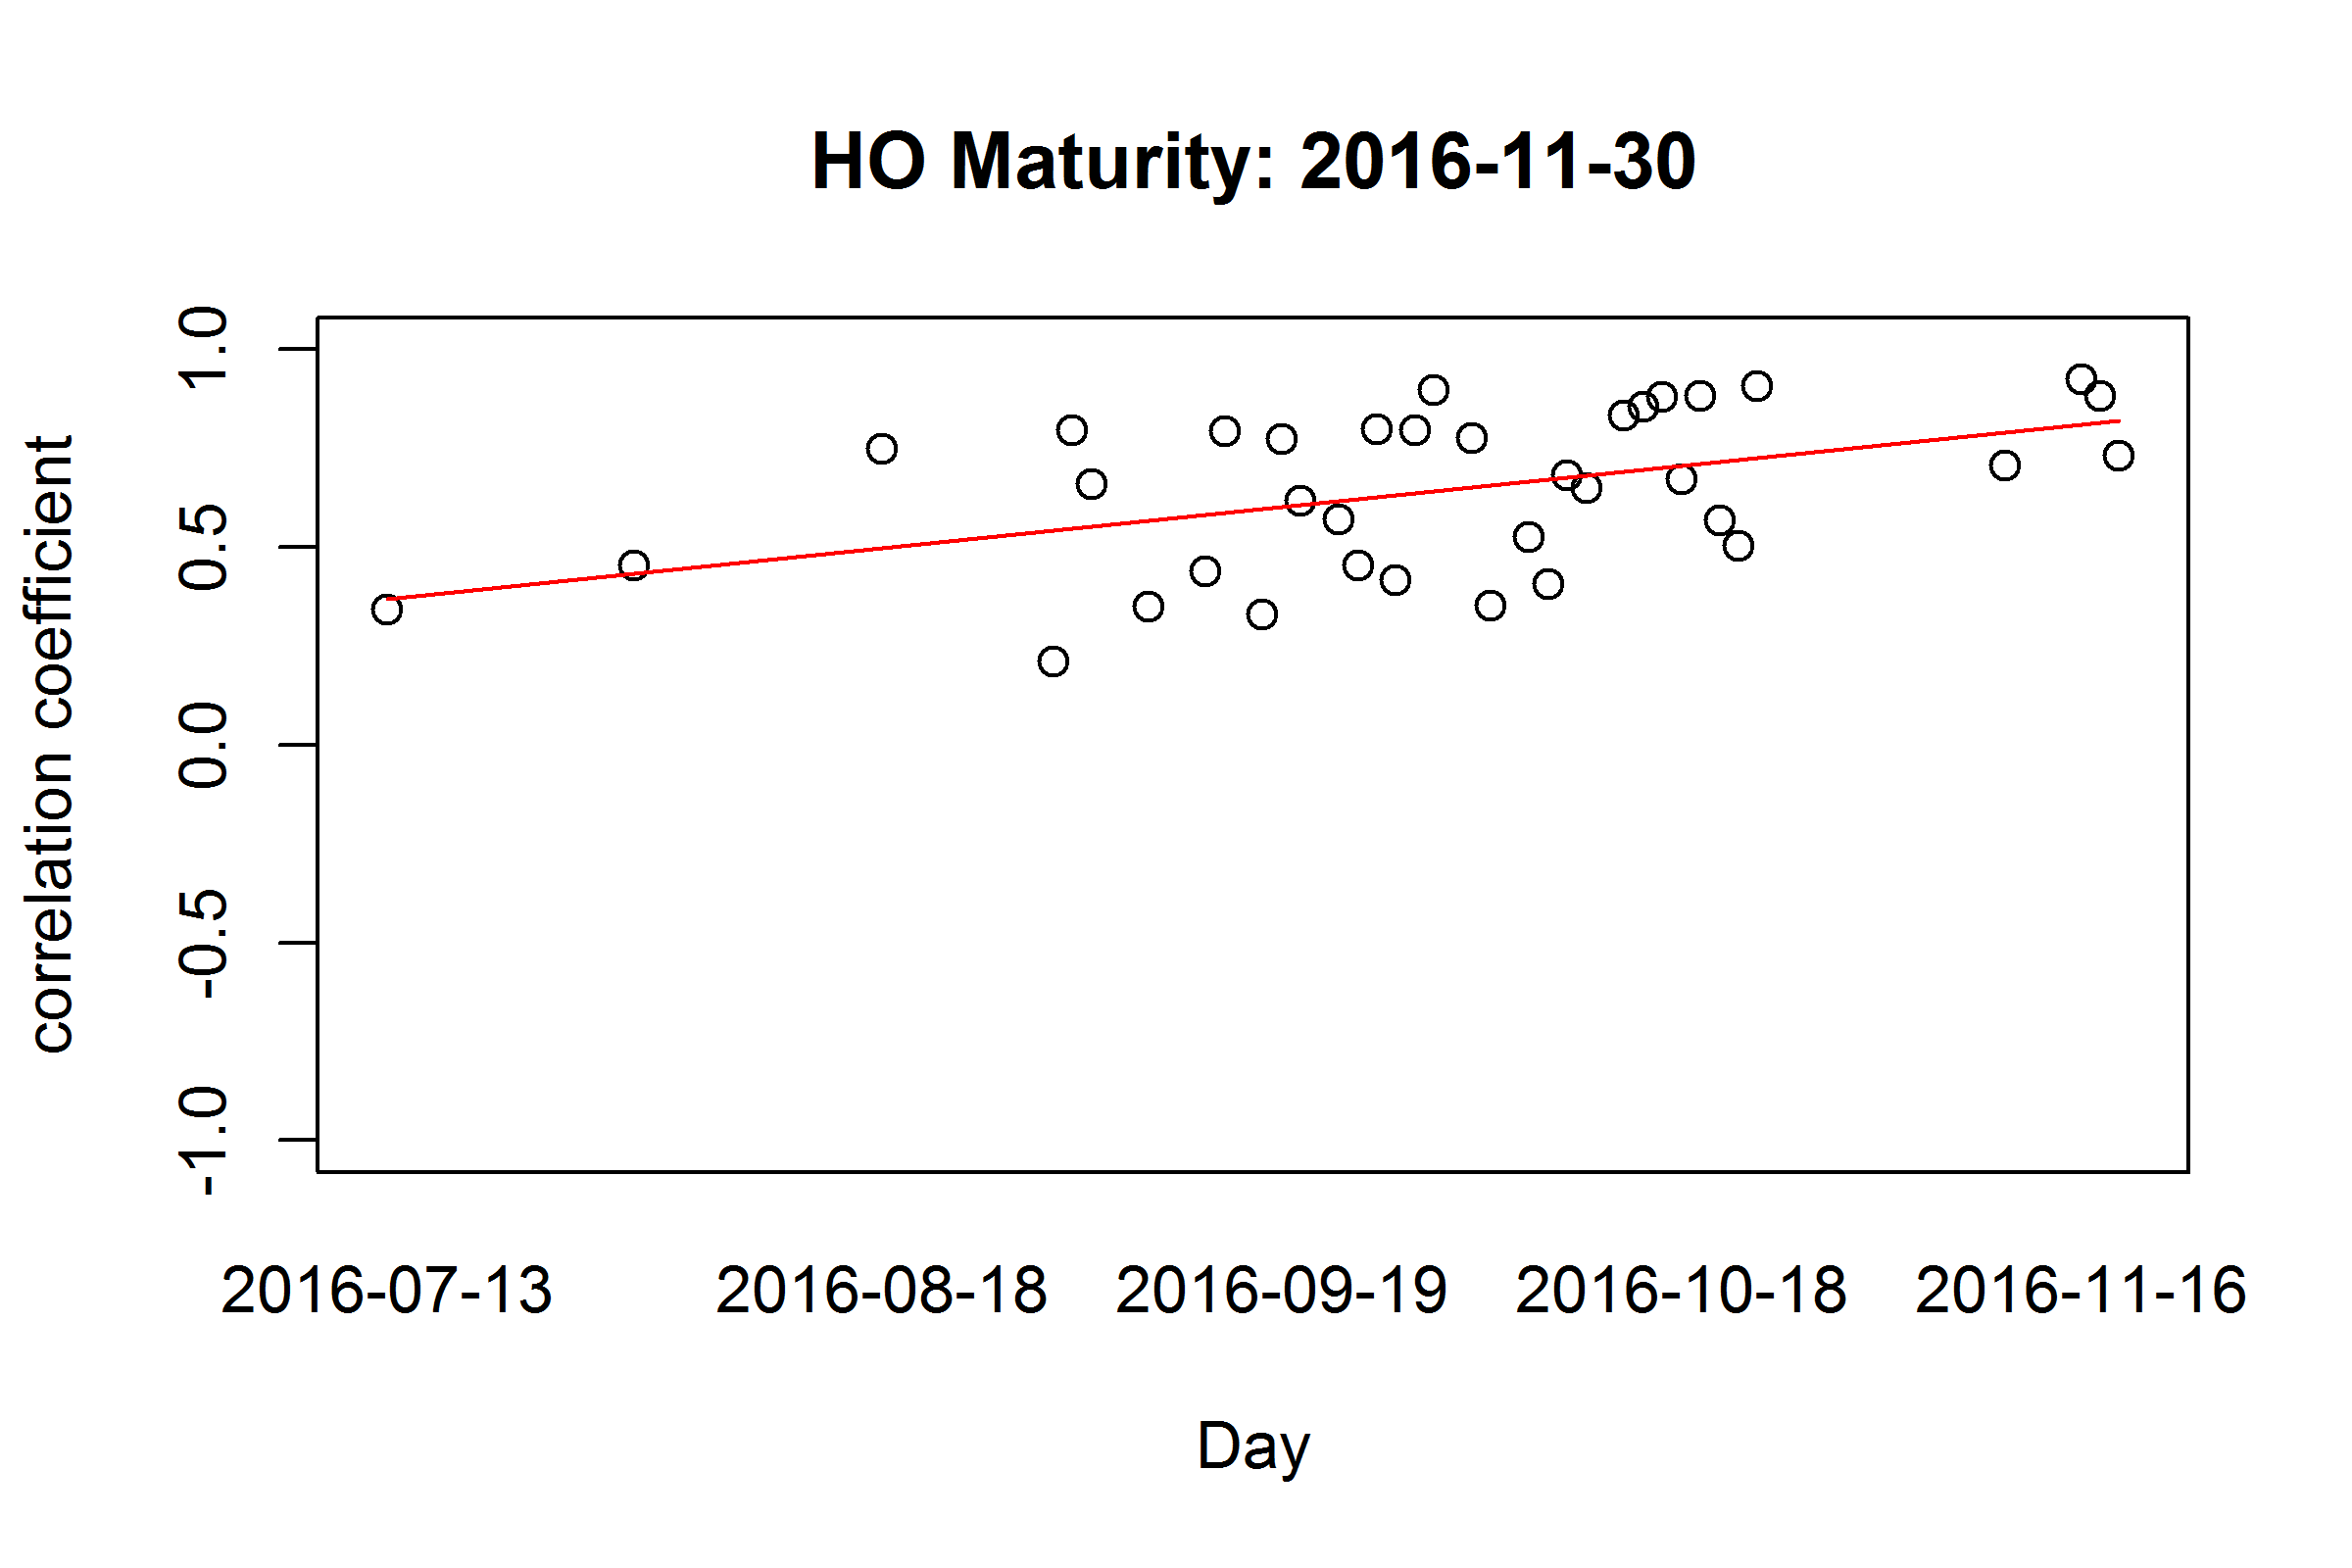
\includegraphics[width=8cm]{Coeff_fitHO2016-11-30.png} &
			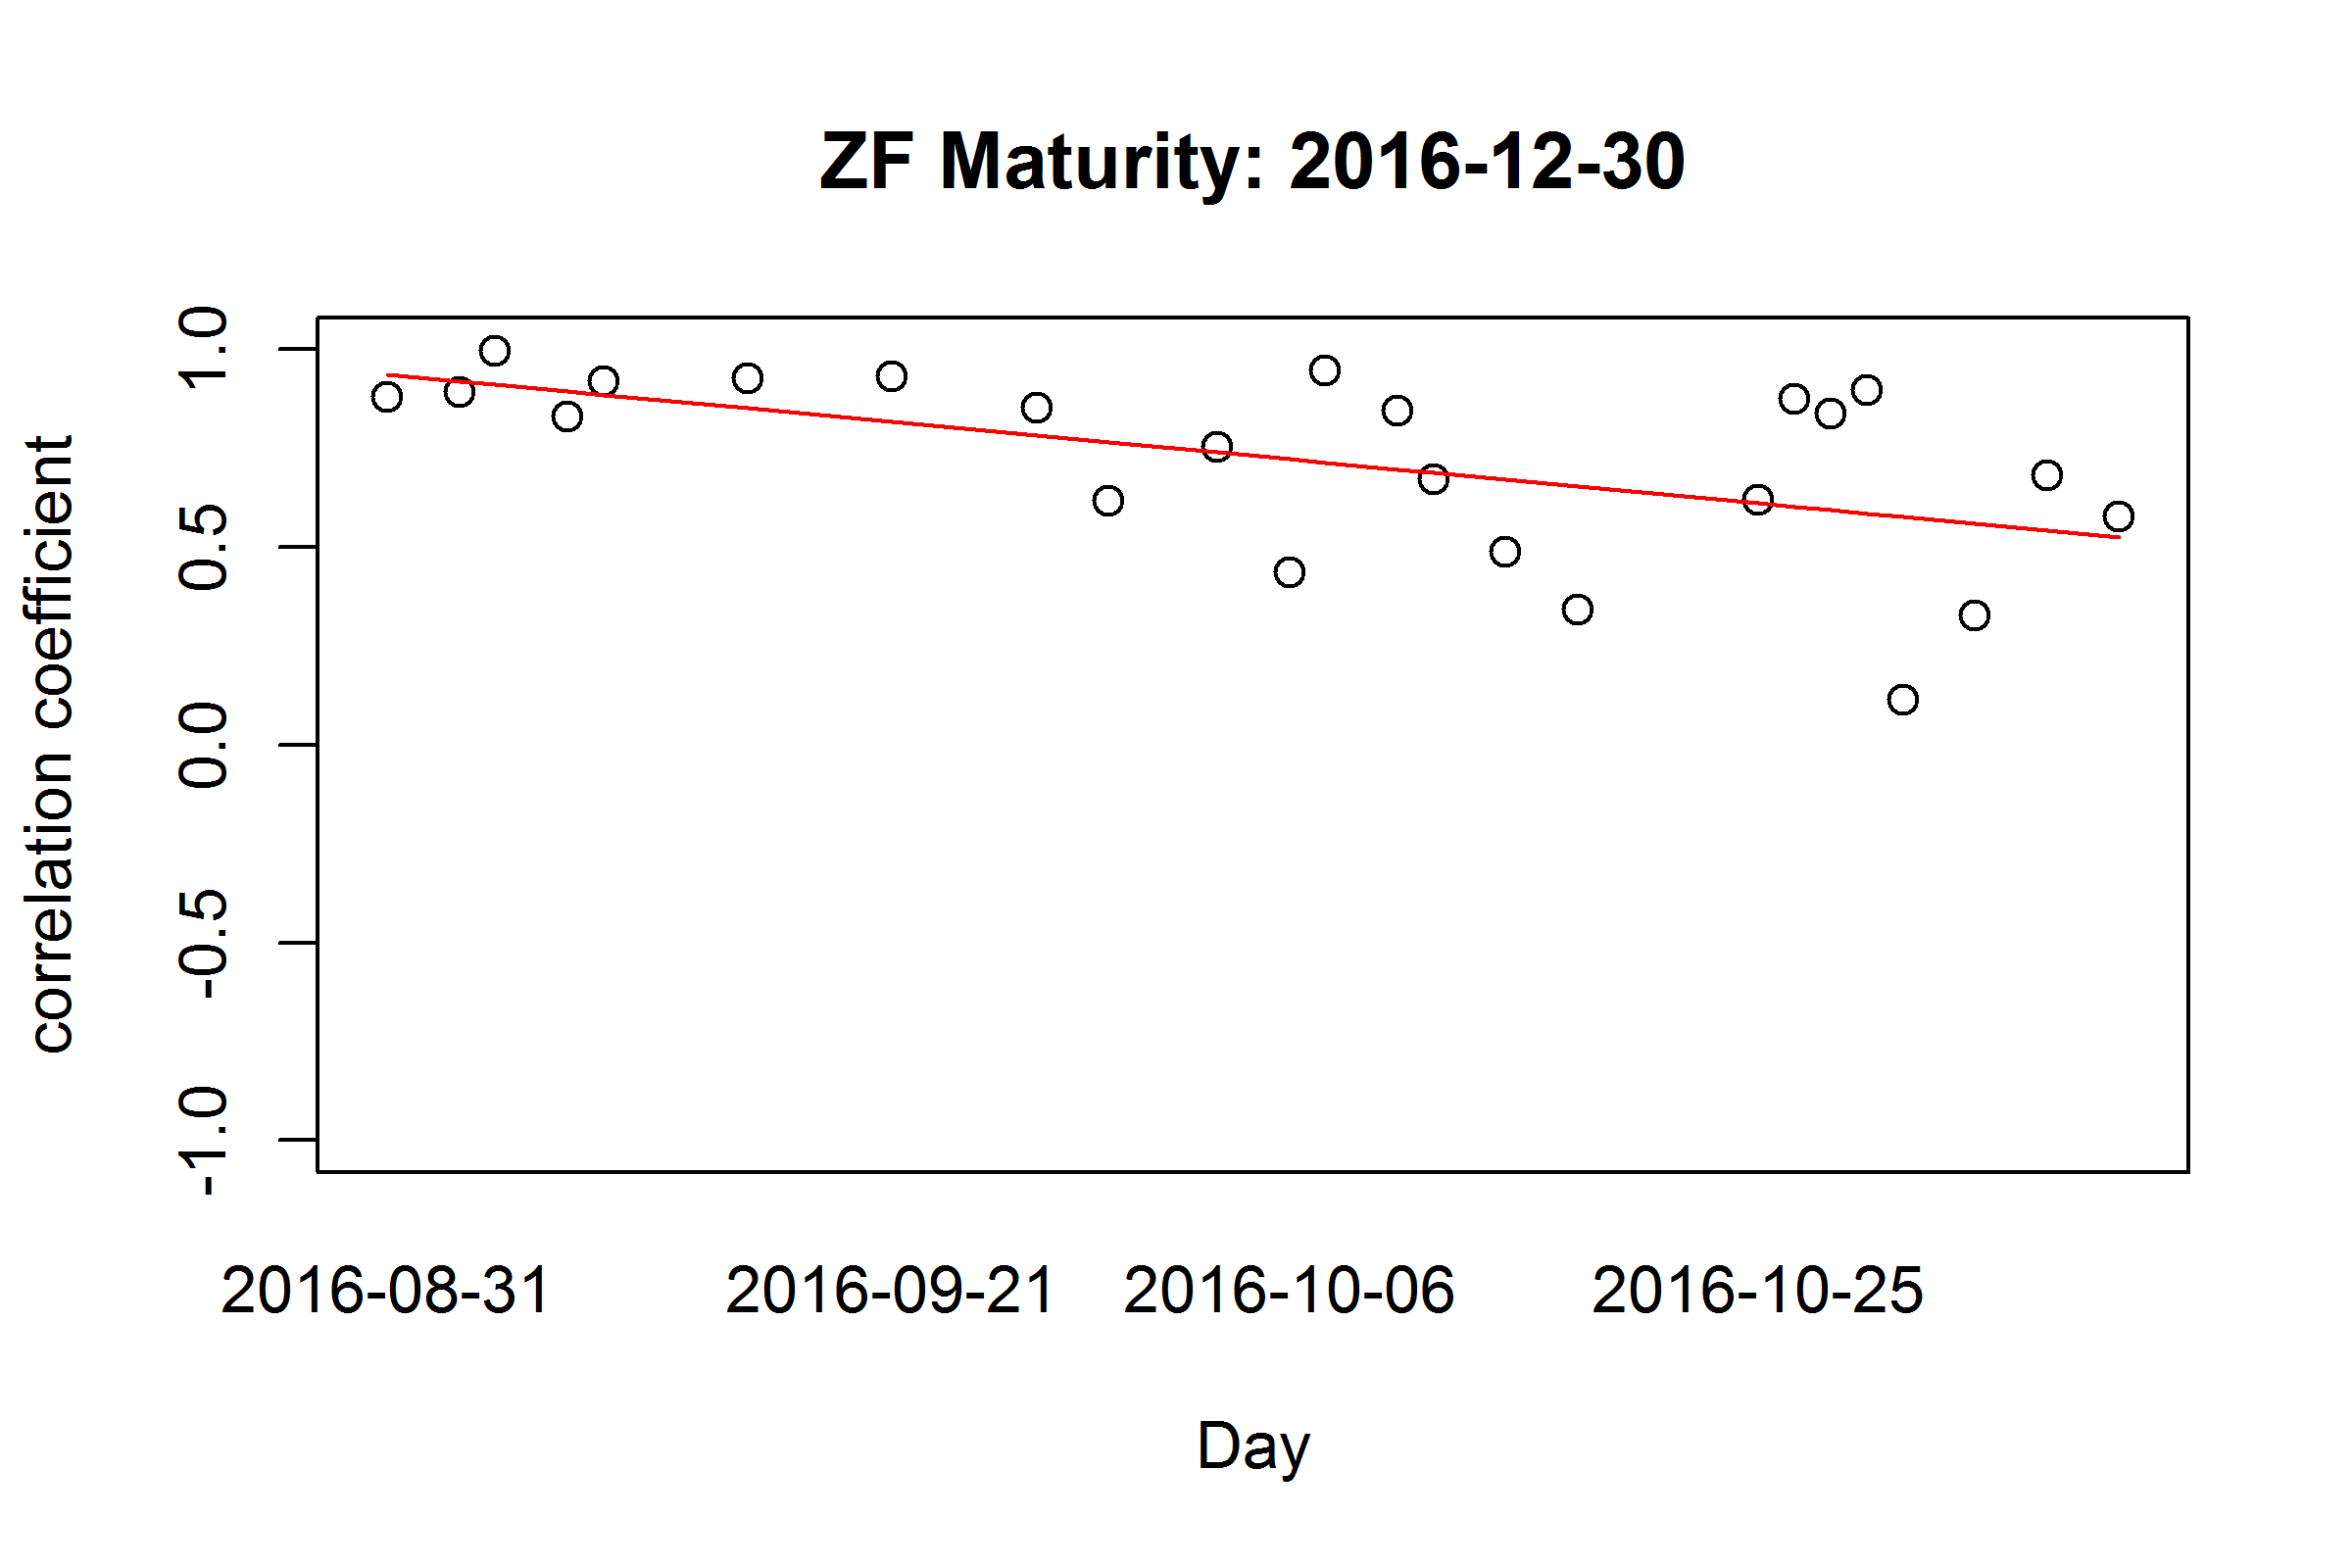
\includegraphics[width=8cm]{Coeff_fitZF2016-12-30.png}\\
			\multicolumn{2}{c}{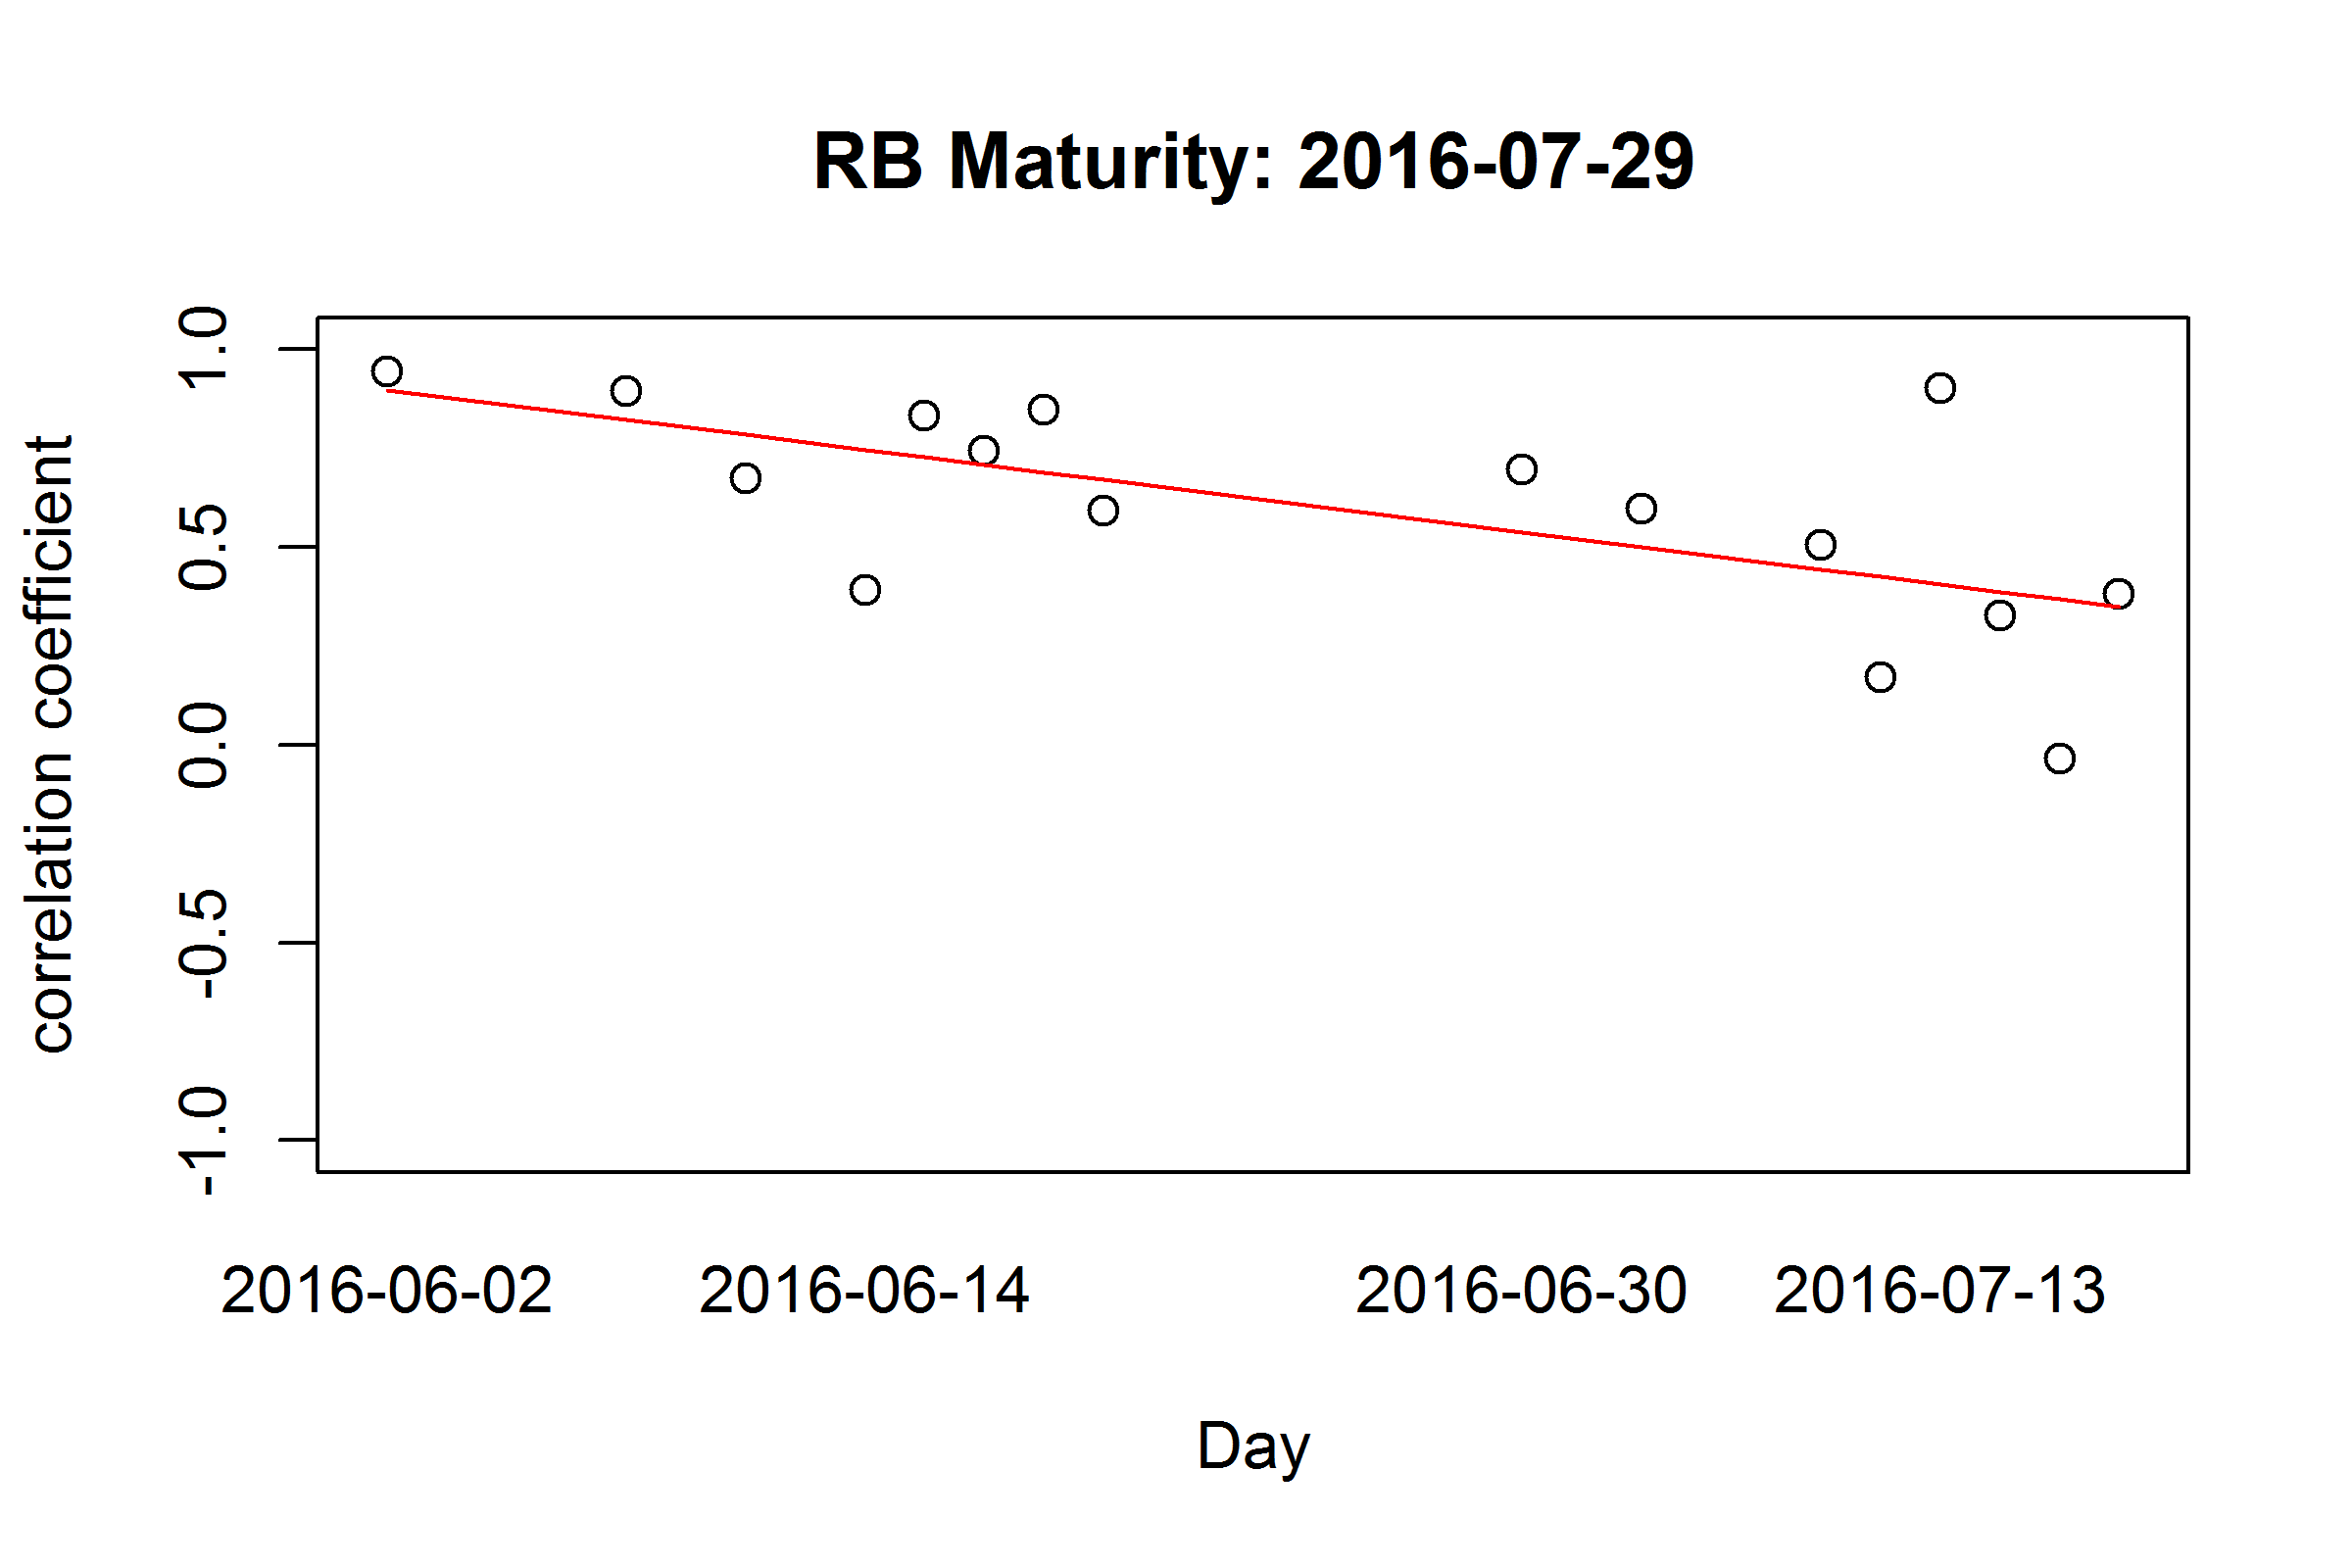
\includegraphics[width=8cm]{Coeff_fitRB2016-07-29.png}}
		\end{tabular}
	\end{center}
	\caption{Correlation regression plots for most significant products}
	\label{fig:10}
\end{figure}

Most products manifested the positive correlation expected between price volatility and trade volume as in Figure 11. The relationship, whether measurements were made hourly or daily, was also consistent for the most part. However, some plots (Figures 12 to 17) either deviated from each other when daily and hourly measurements were compared or did not exhibit the expectation of a positive correlation.

\begin{figure}[H]
	\begin{center}
		\begin{tabular}{ll}
			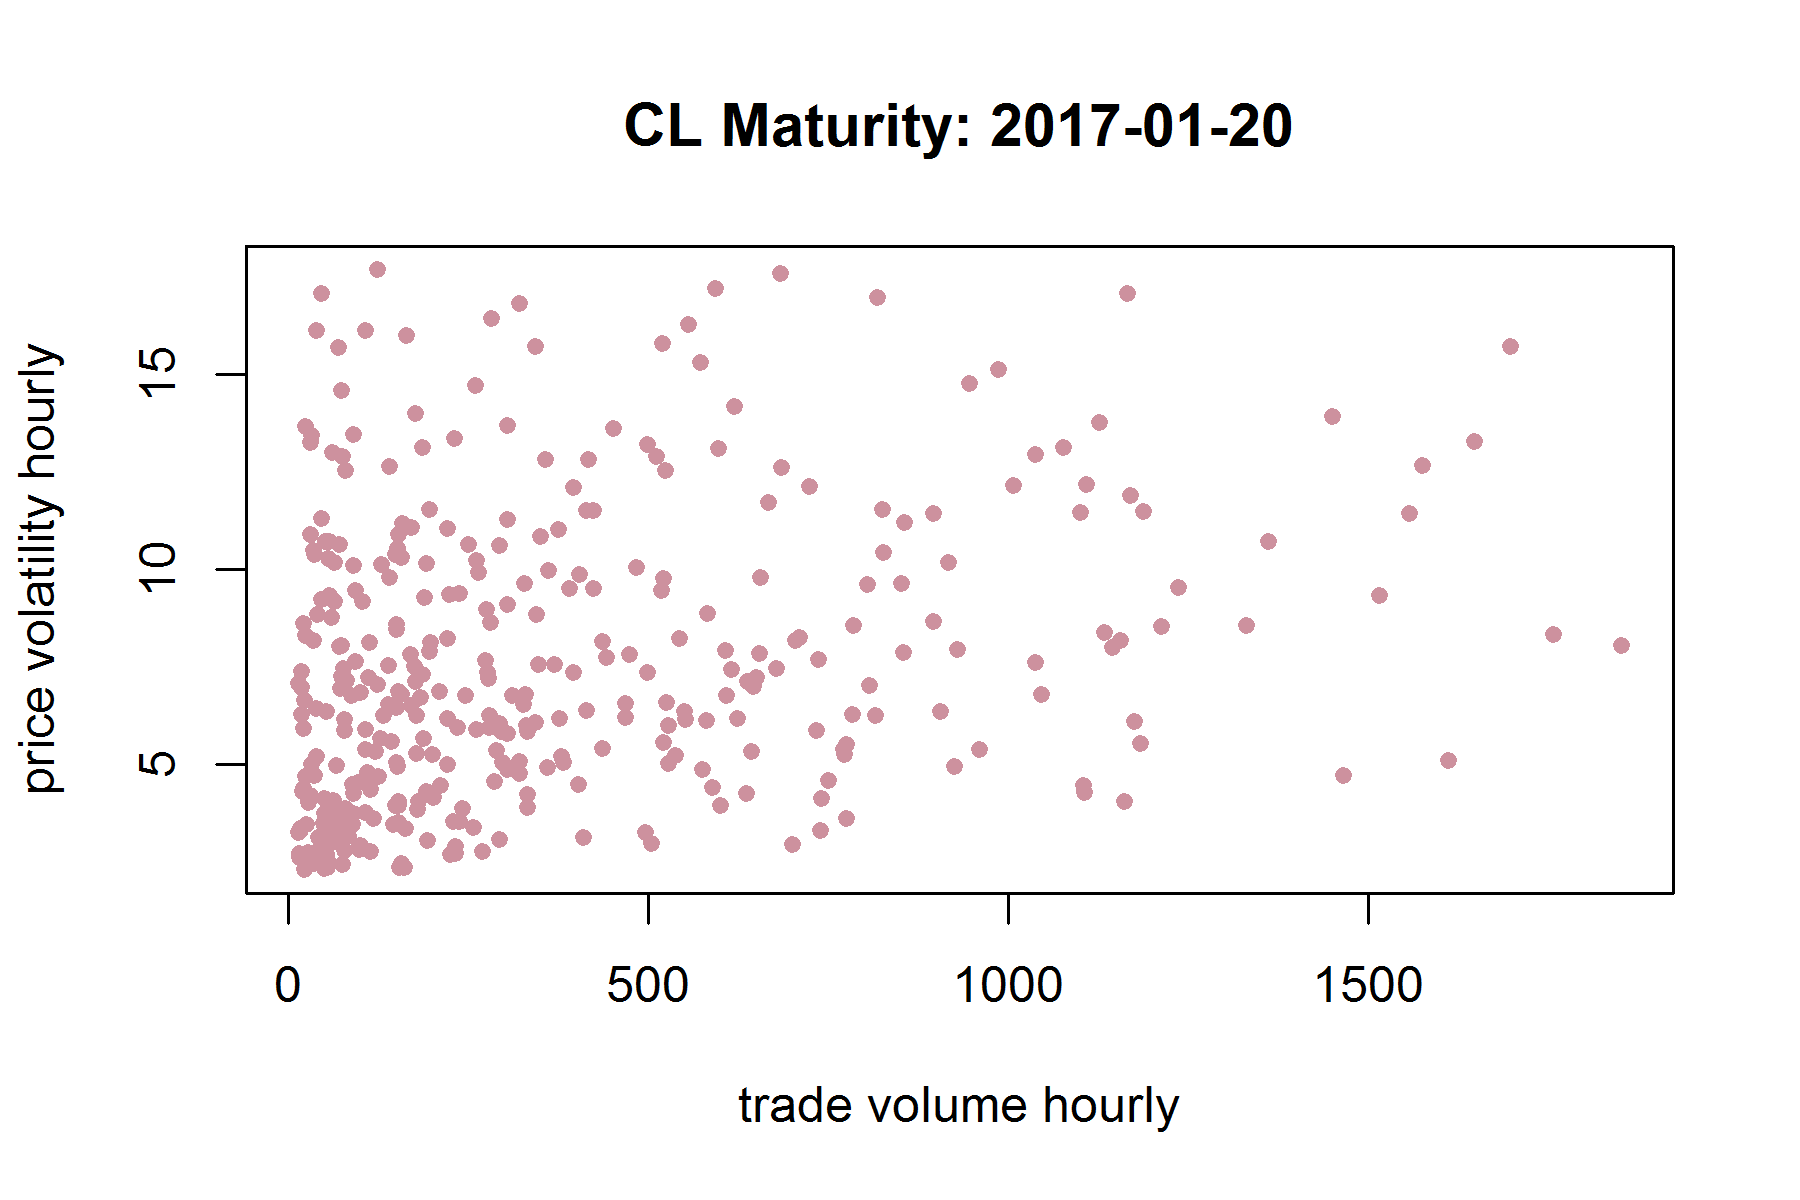
\includegraphics[width=8cm]{CL2017-01-20hourly.png} &
			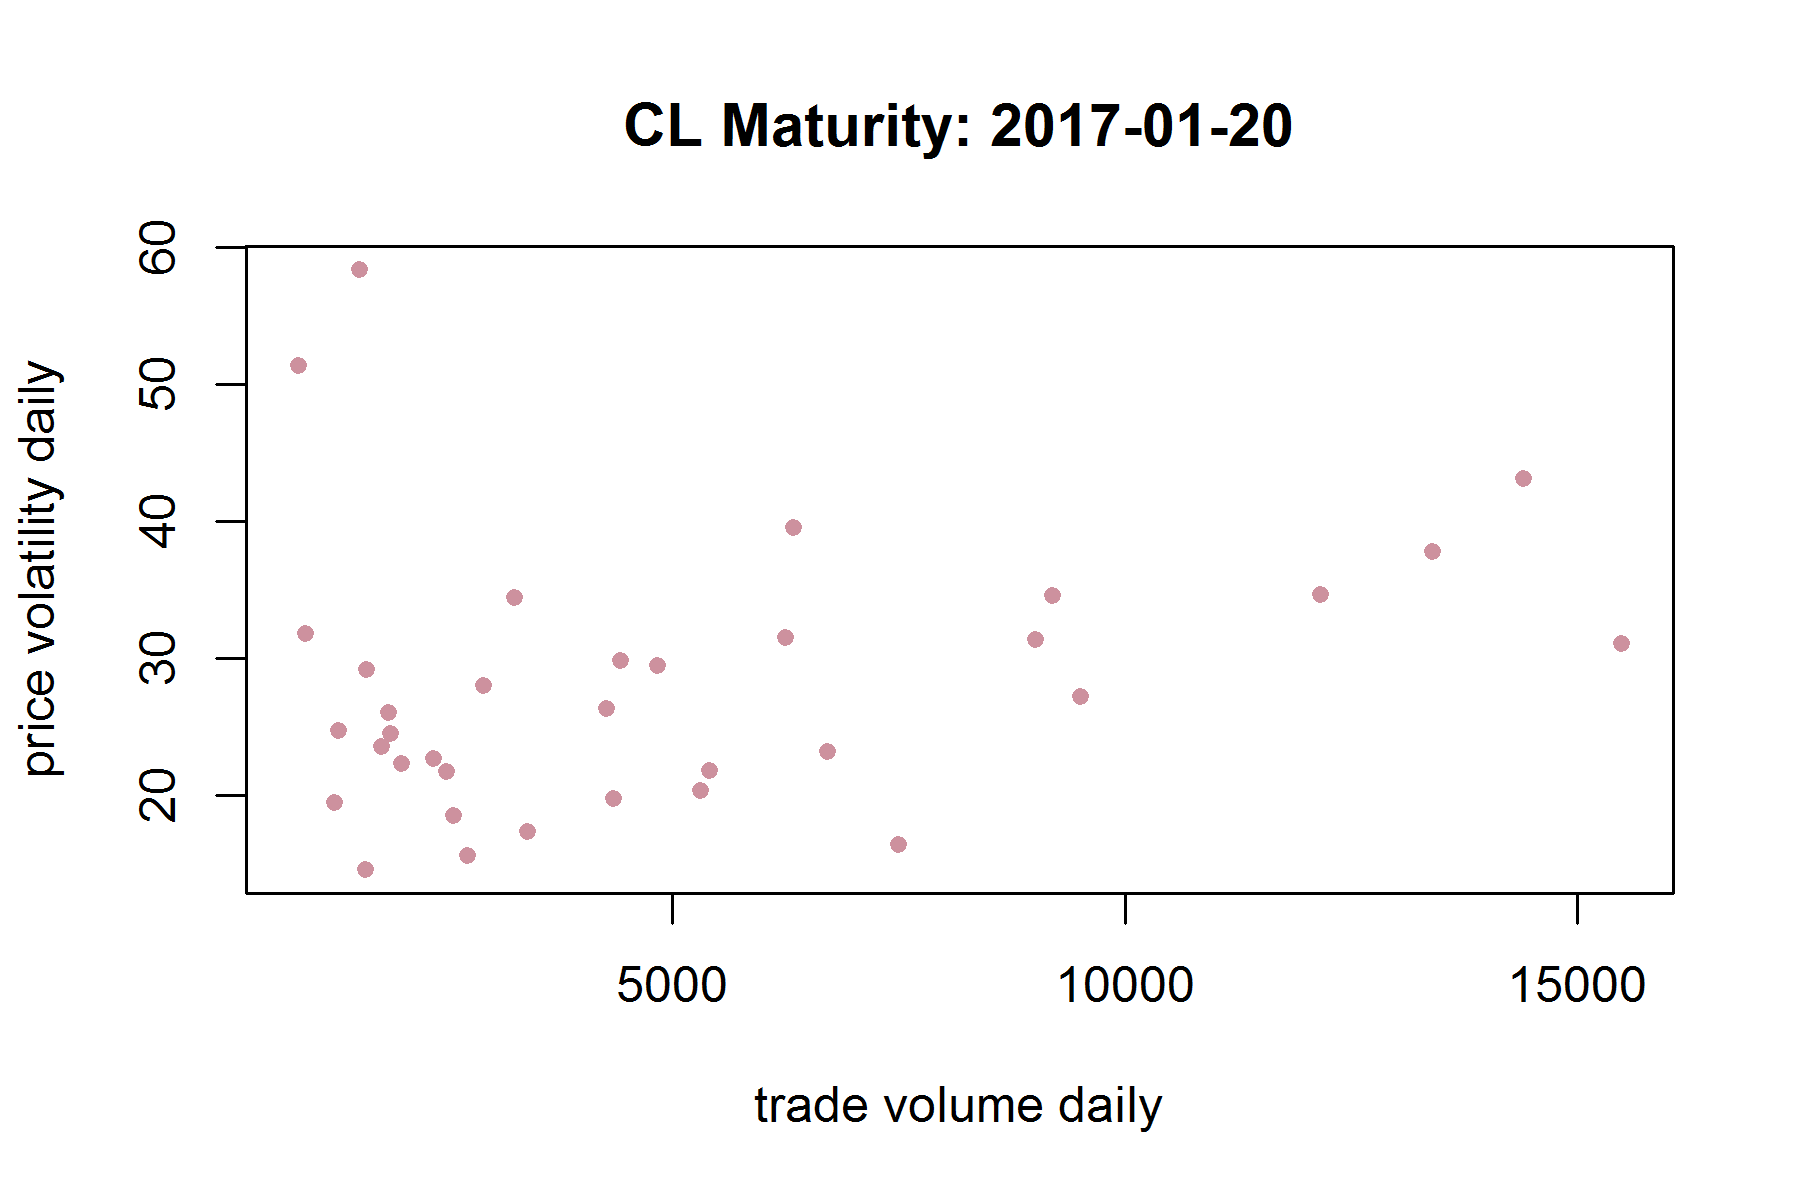
\includegraphics[width=8cm]{CL2017-01-20daily.png} \\
		\end{tabular}
	\end{center}
	\caption{Price volatility vs. trade volume shows positive correlation}
	\label{fig: 11}
\end{figure}

\begin{figure}[H]
	\begin{center}
		\begin{tabular}{ll}
		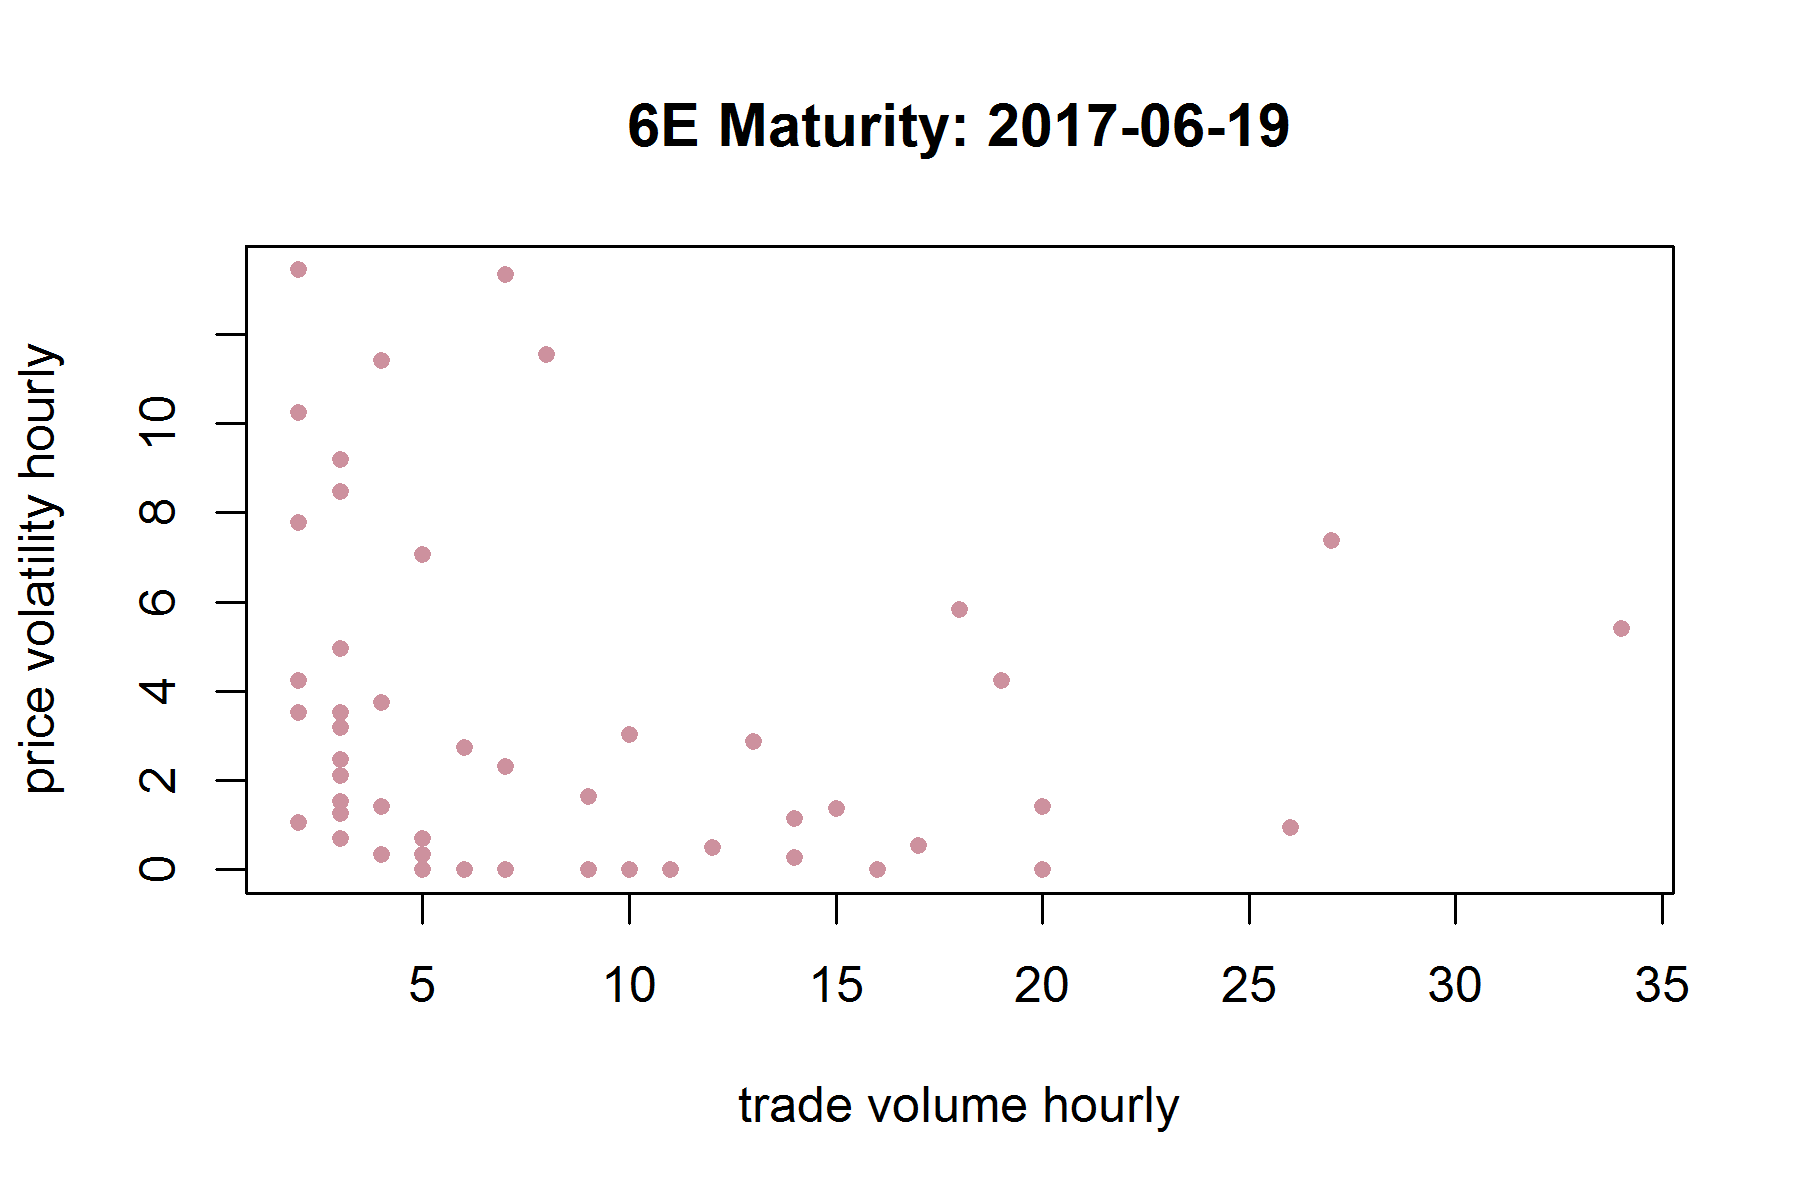
\includegraphics[width=8cm]{6E2017-06-19hourly.png} &
		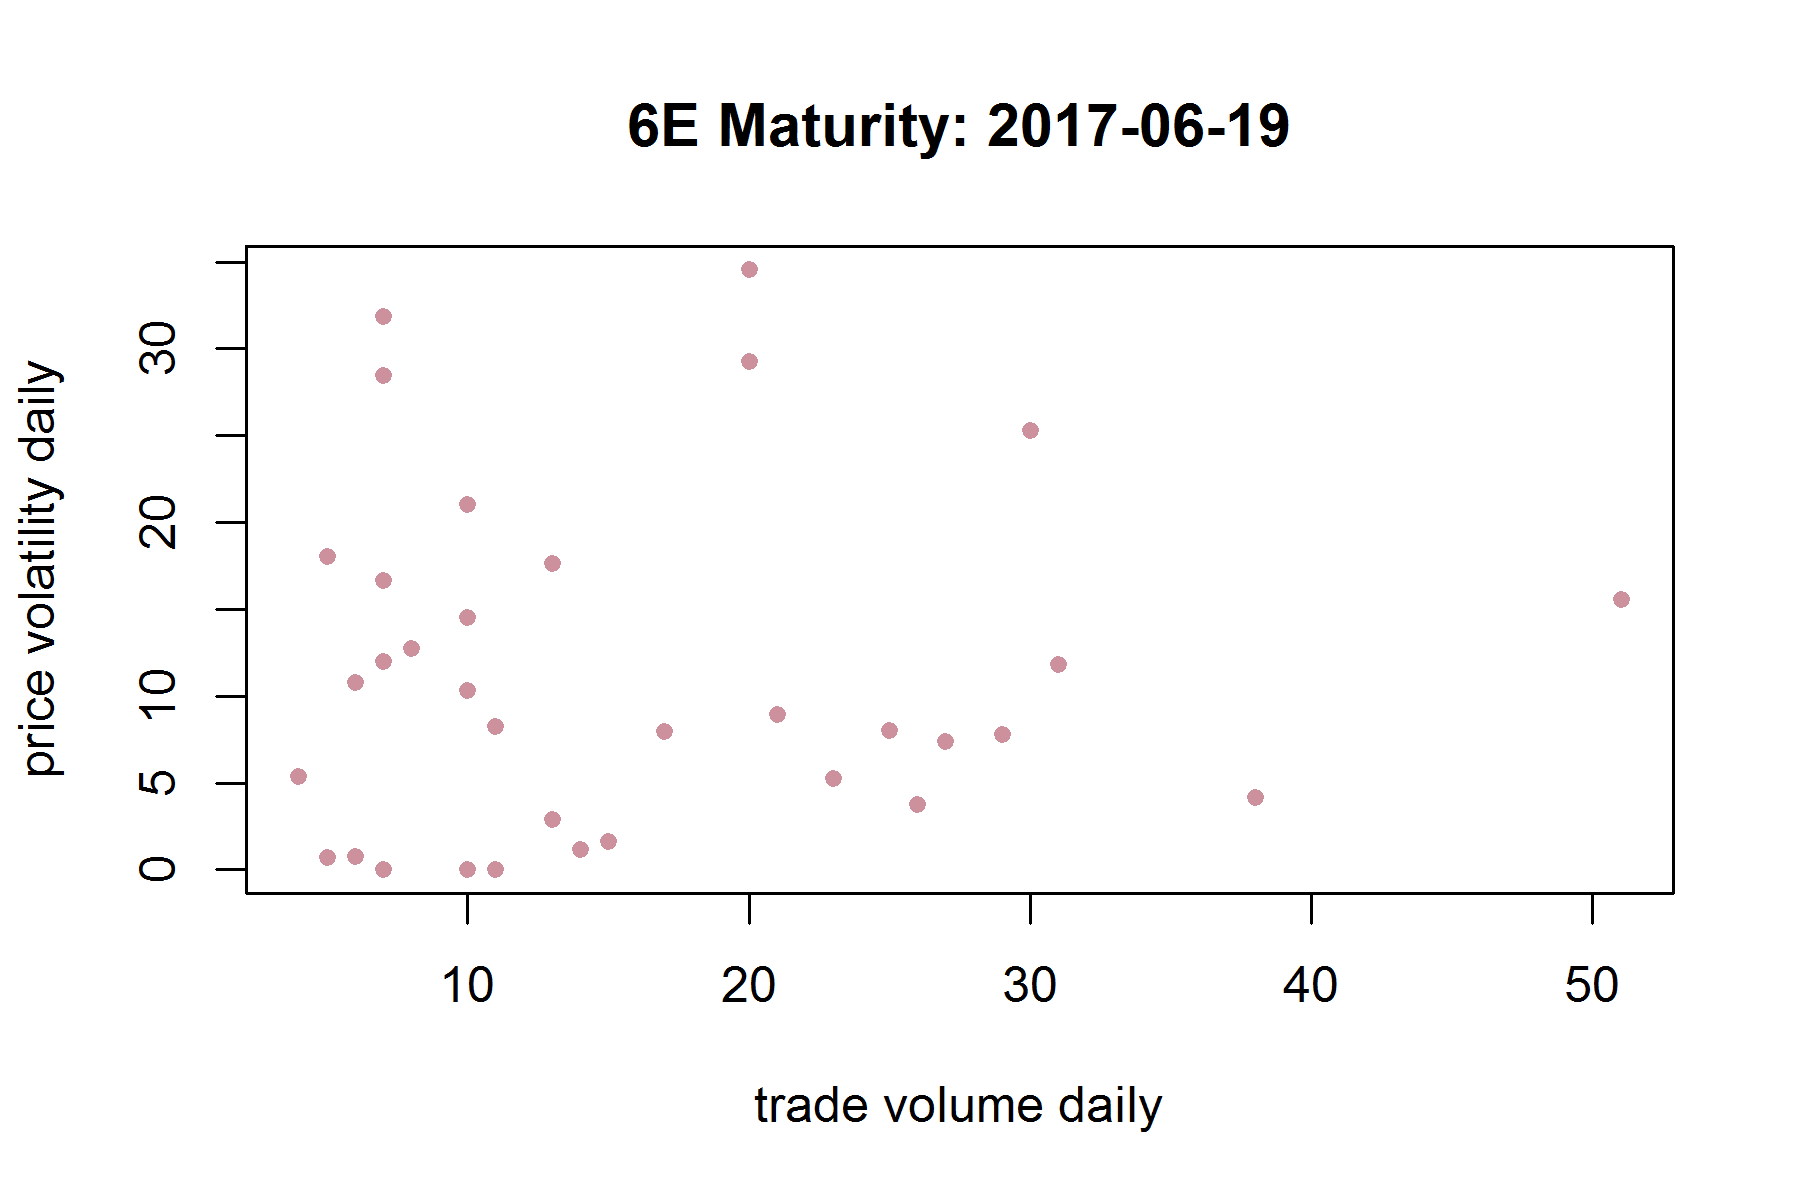
\includegraphics[width=8cm]{6E2017-06-19daily.png} \\
		\end{tabular}
	\end{center}
		\caption{Price volatility vs. trade volume shows negative correlation}
		\label{fig: 12}
\end{figure}

\begin{figure}[H]
	\begin{center}
		\begin{tabular}{ll}
			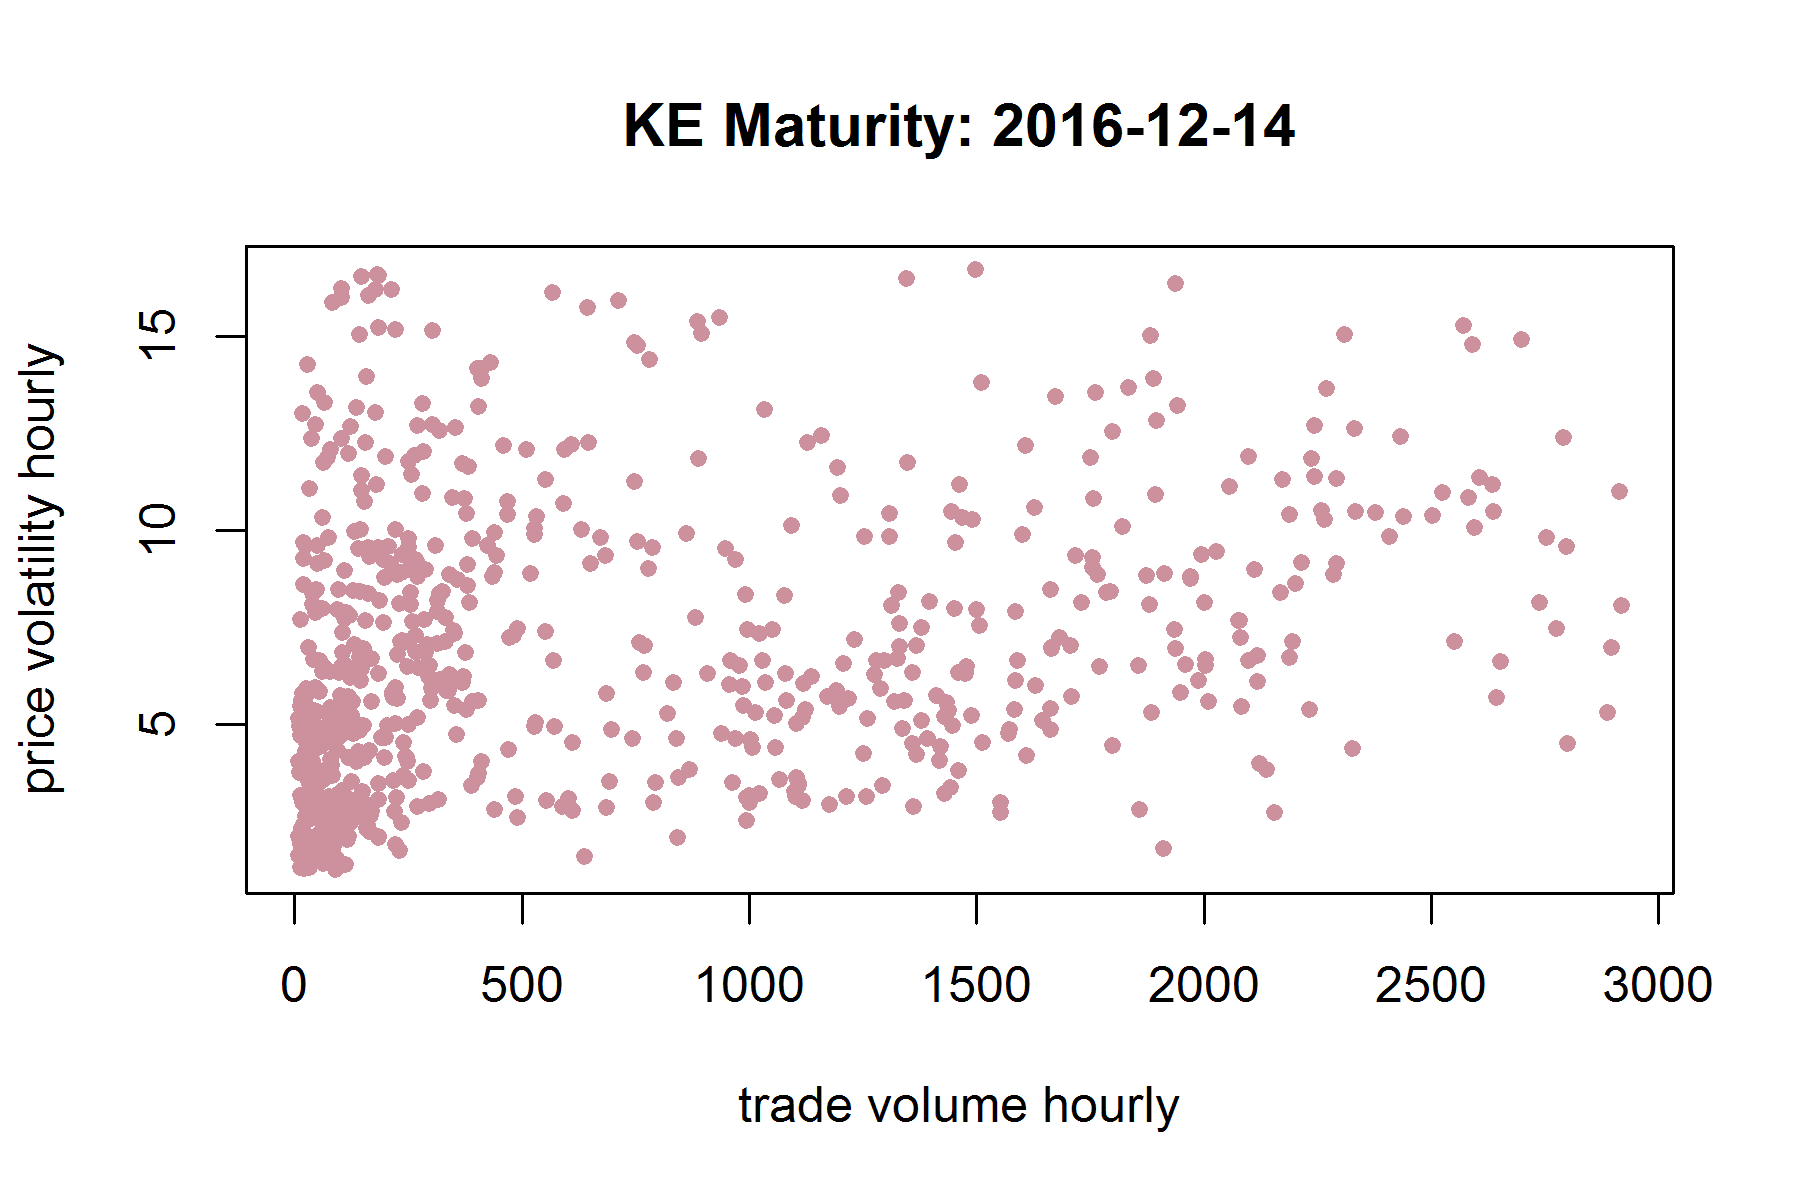
\includegraphics[width=8cm]{KE2016-12-14hourly.png} &
			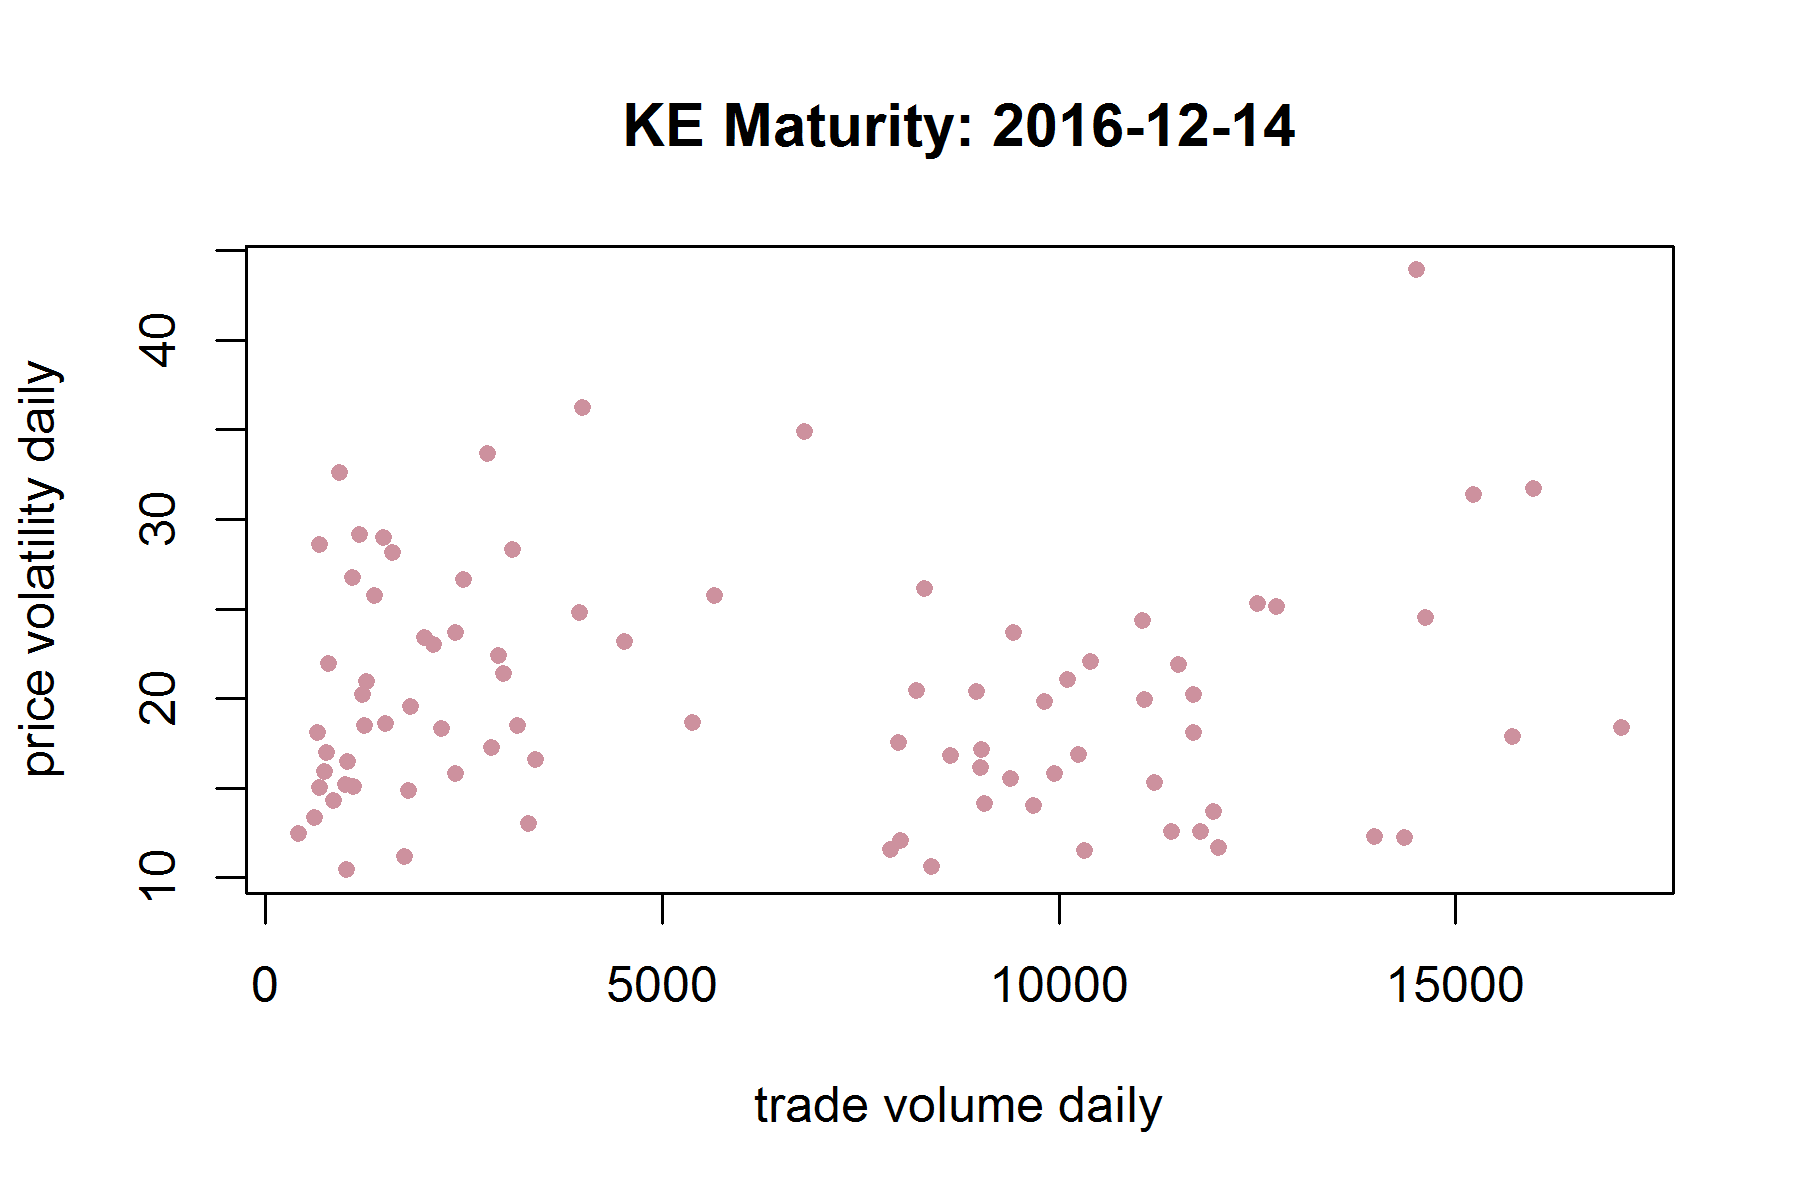
\includegraphics[width=8cm]{KE2016-12-14daily.png} \\
		\end{tabular}
	\end{center}
	\caption{Price volatility vs. trade volume shows two clusters}
	\label{fig: 13}
\end{figure}


\begin{figure}[H]
	\begin{center}
		\begin{tabular}{ll}
			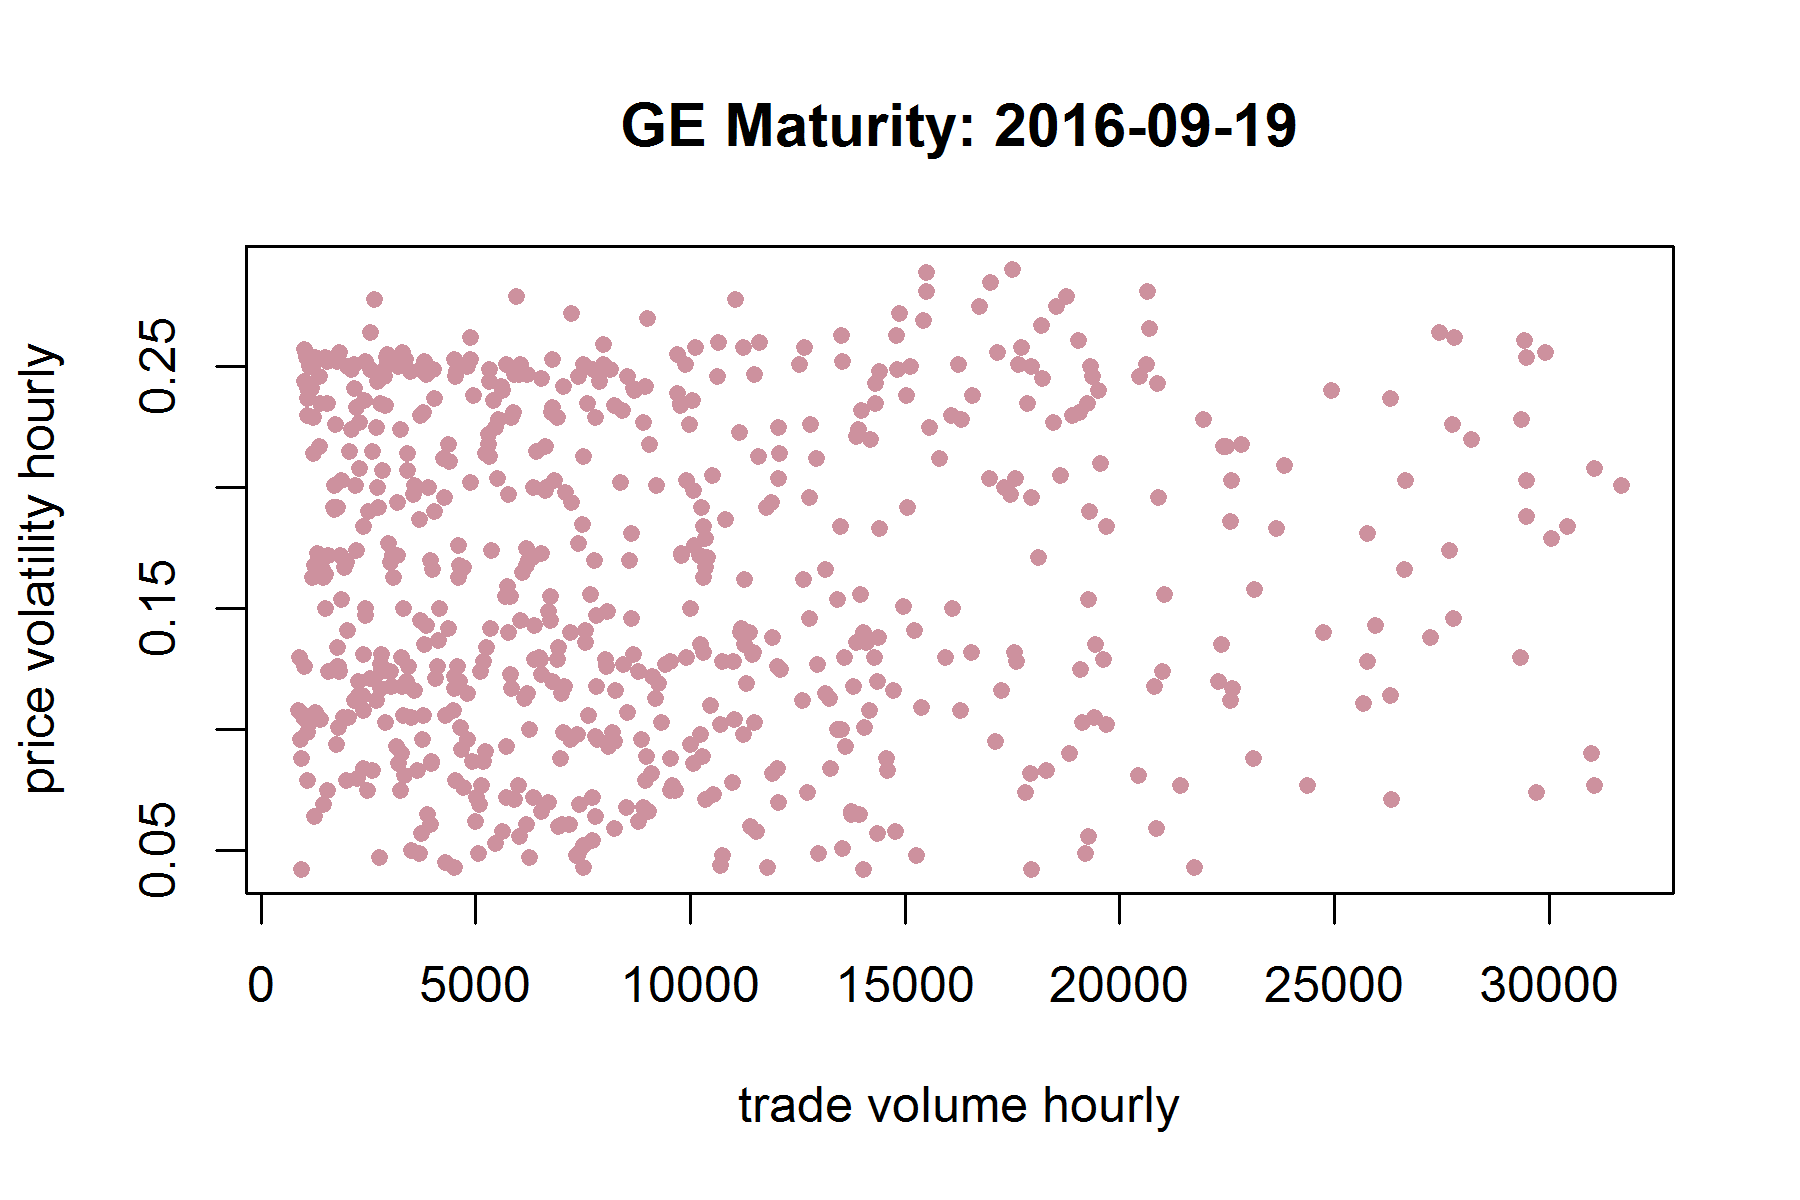
\includegraphics[width=8cm]{GE2016-09-19hourly.png} &
			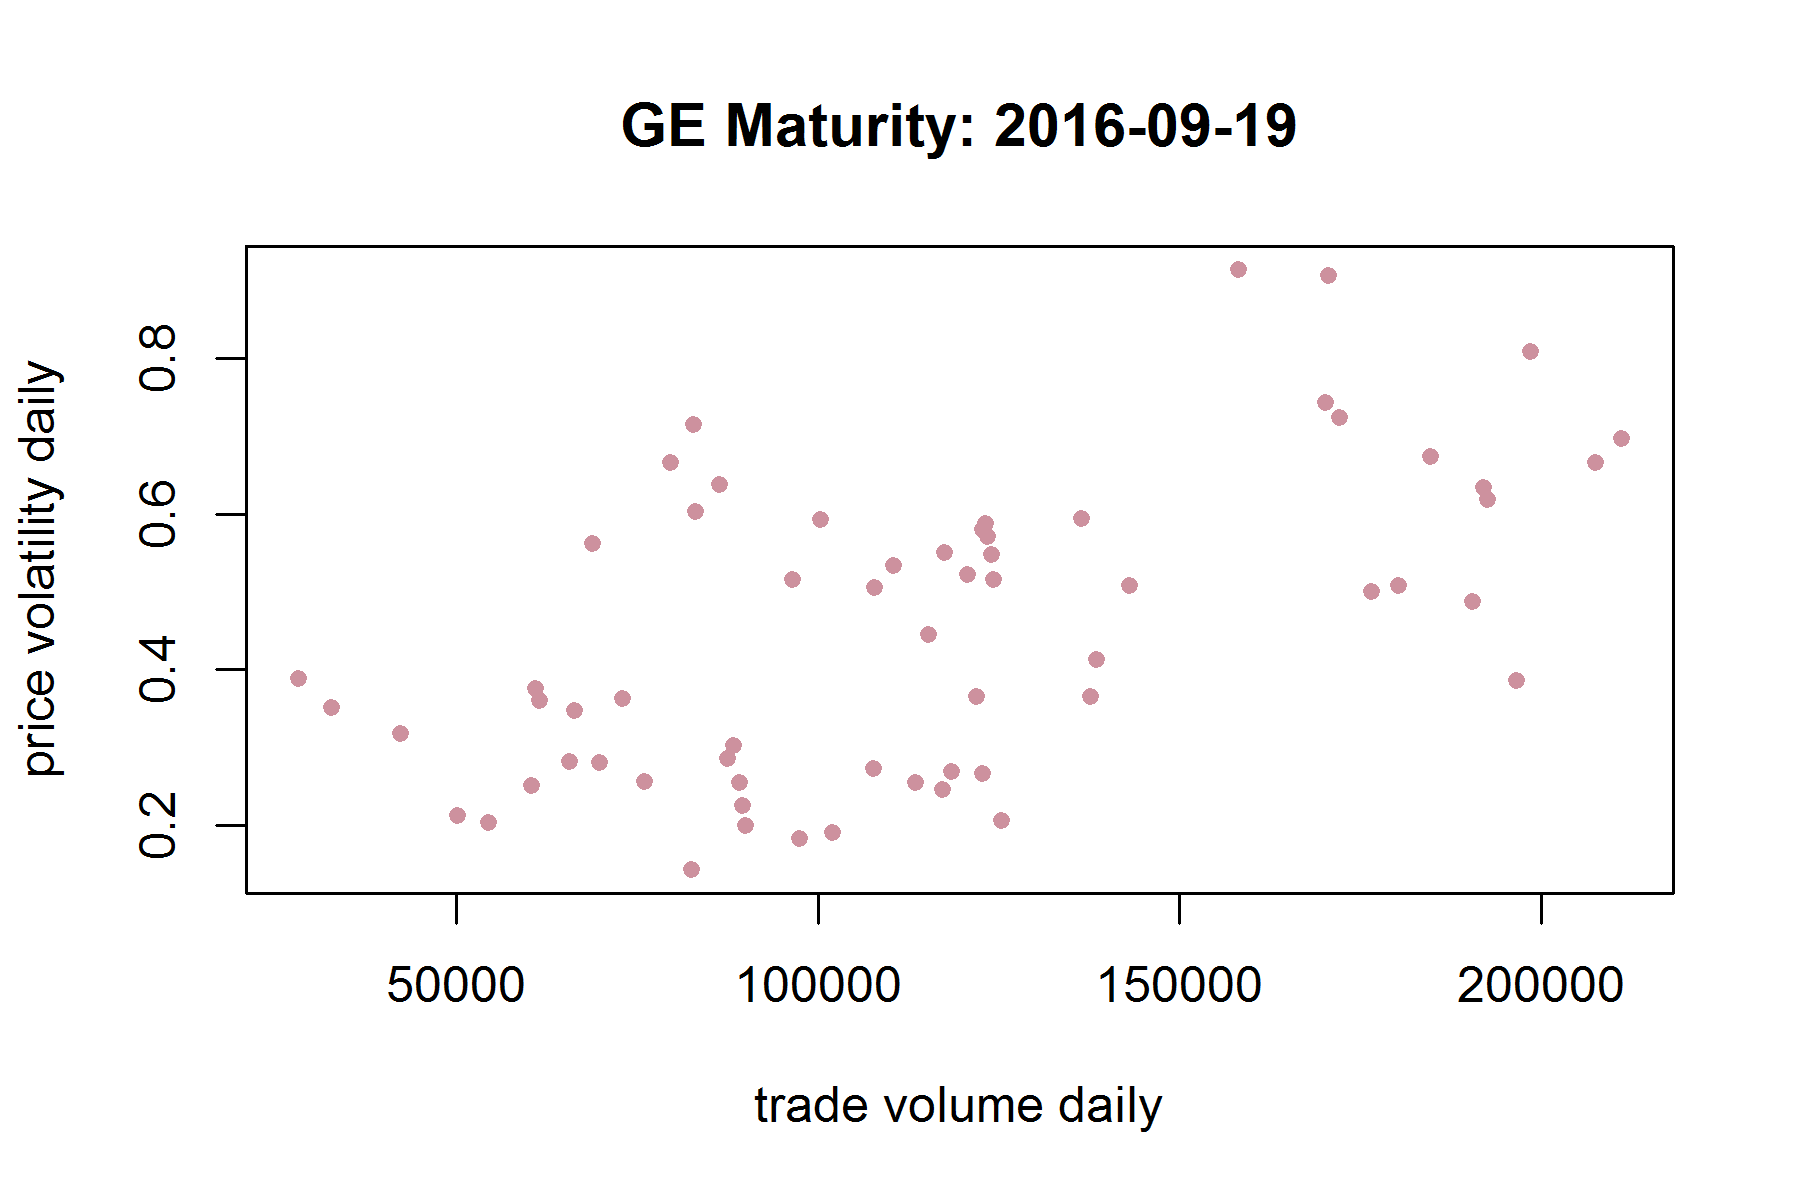
\includegraphics[width=8cm]{GE2016-09-19daily.png} \\
		\end{tabular}
	\end{center}
	\caption{Price volatility vs. trade volume hourly \& daily show different correlations}
	\label{fig: 14}
\end{figure}

\begin{figure}[H]
	\begin{center}
		\begin{tabular}{ll}
			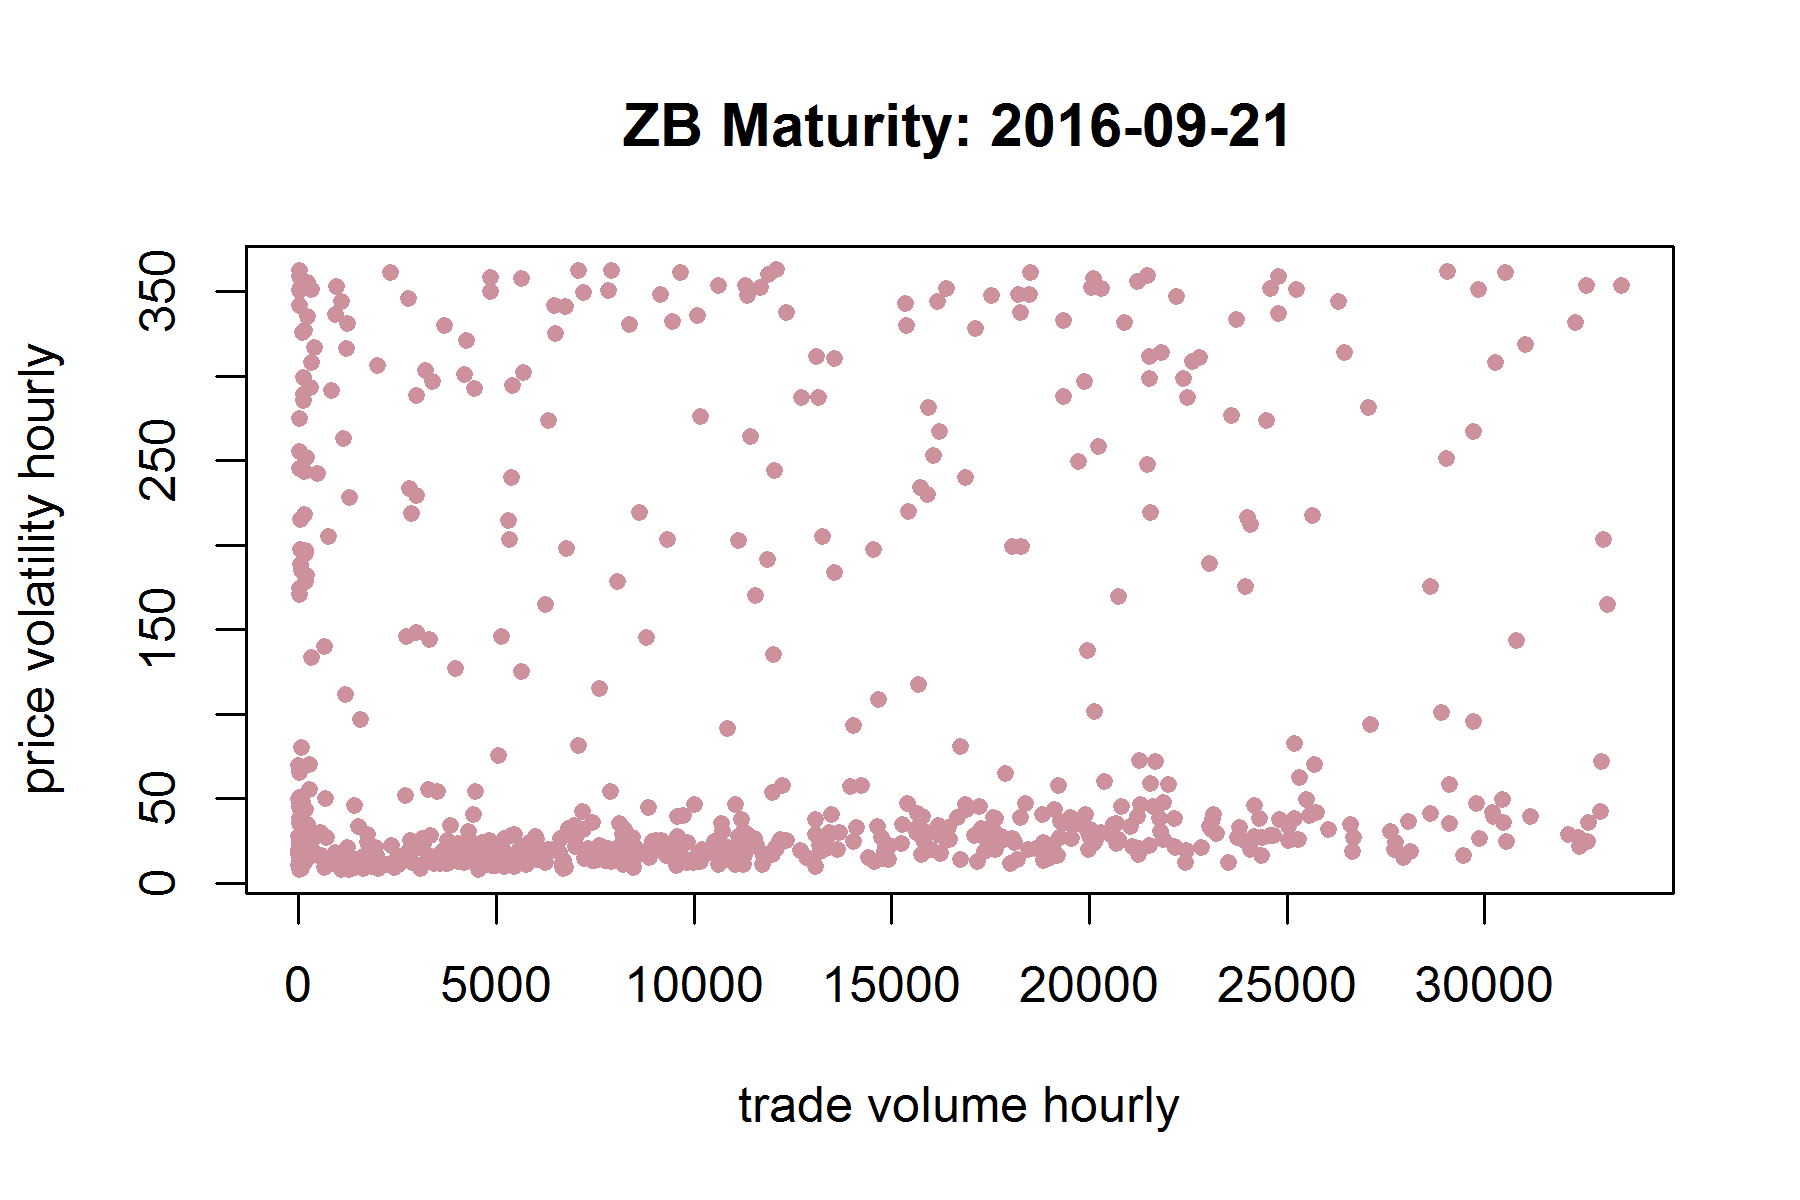
\includegraphics[width=8cm]{ZB2016-09-21hourly.png} &
			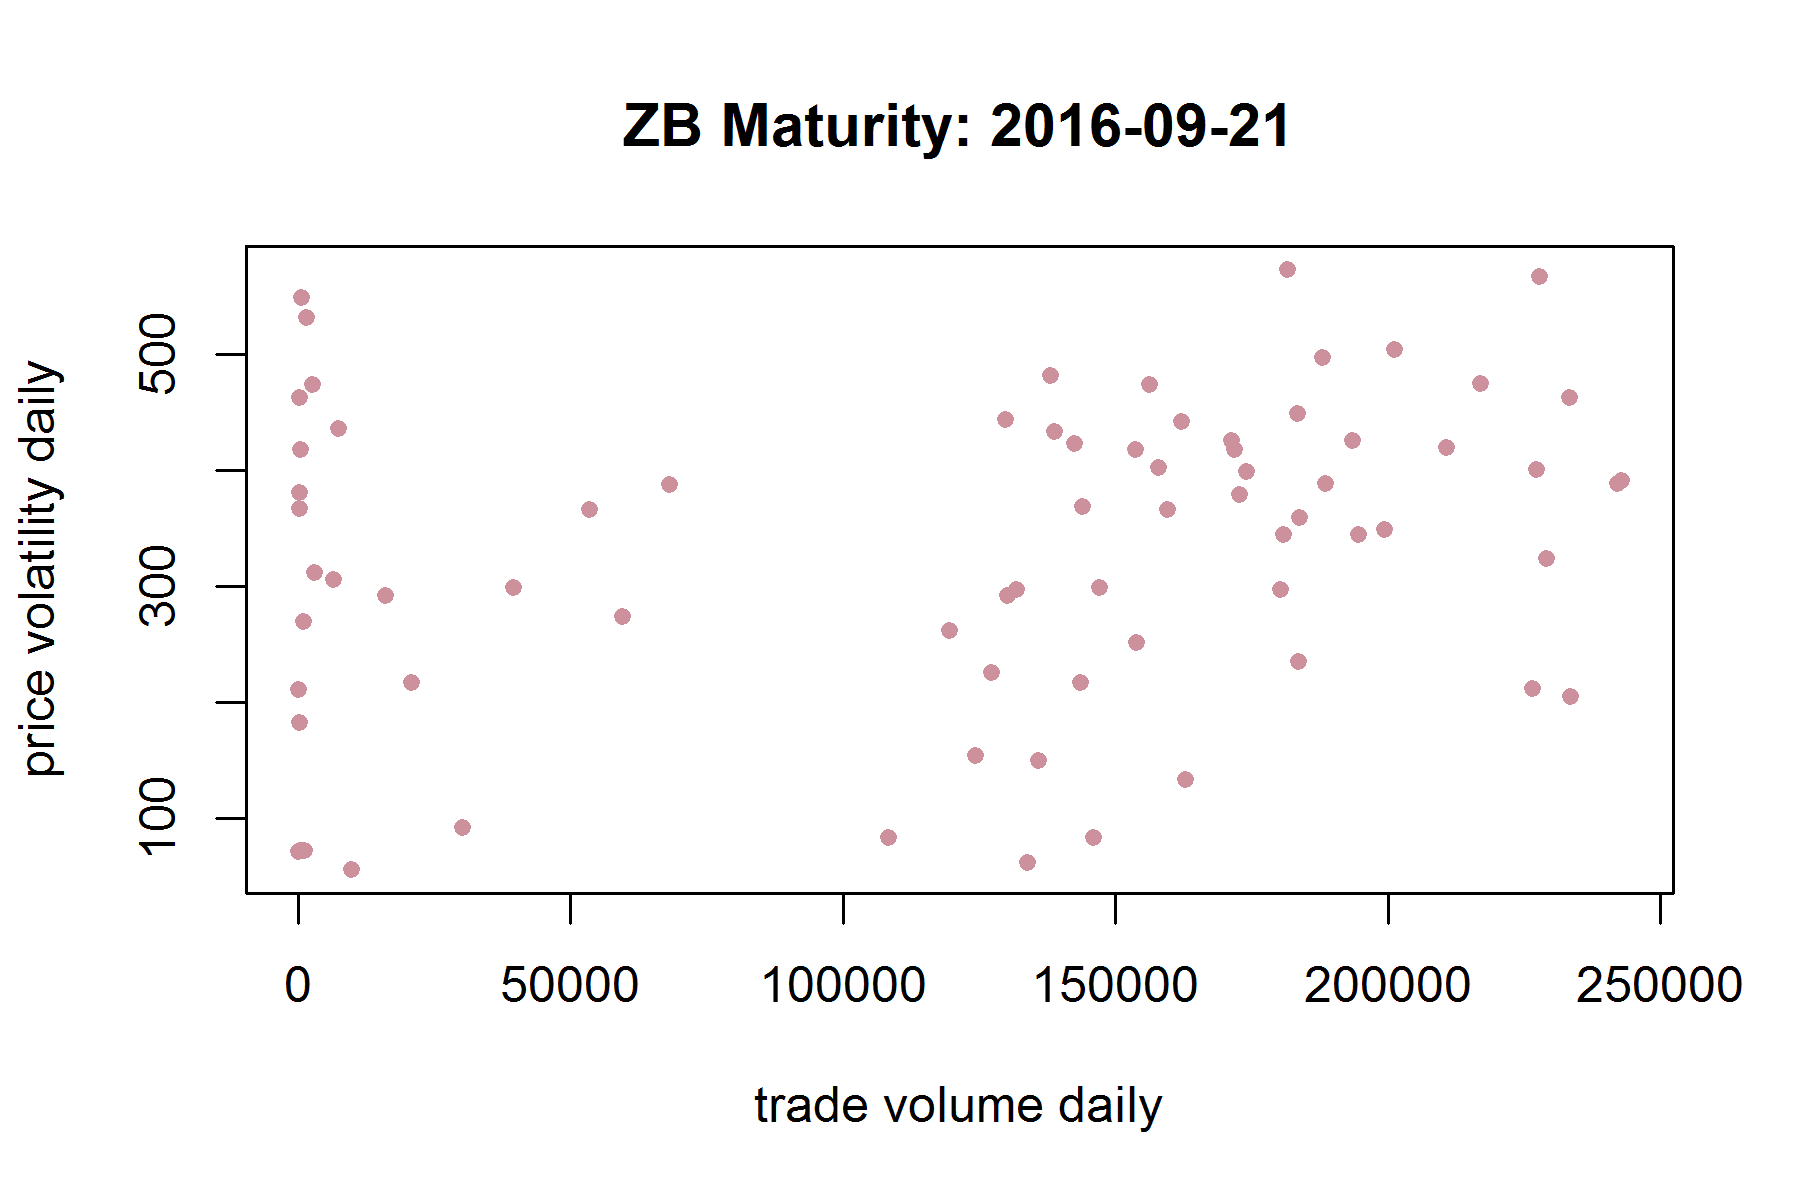
\includegraphics[width=8cm]{ZB2016-09-21daily.png} \\
		\end{tabular}
	\end{center}
	\caption{Price volatility vs. trade volume hourly \& daily show different clusters}
	\label{fig: 15}
\end{figure}

\begin{figure}[H]
	\begin{center}
		\begin{tabular}{ll}
			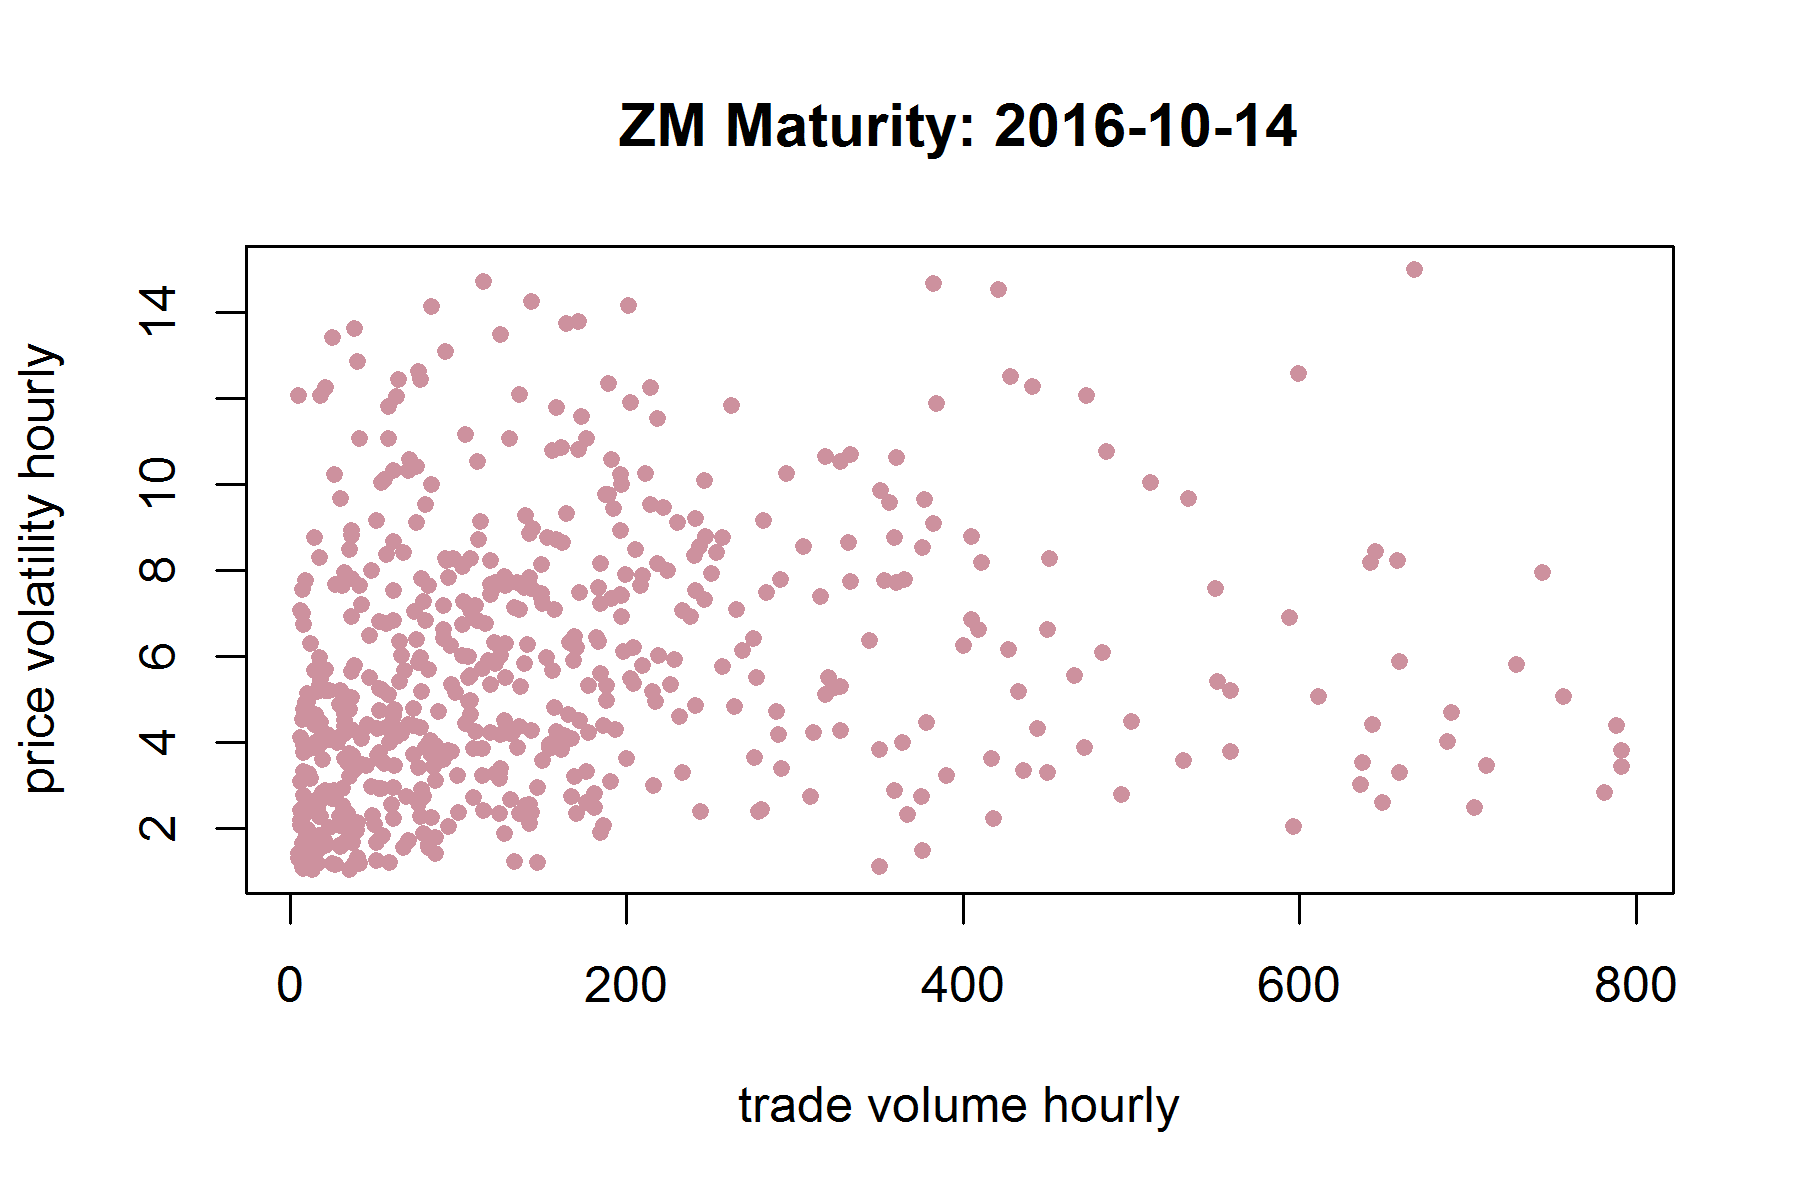
\includegraphics[width=8cm]{ZM2016-10-14hourly.png} &
			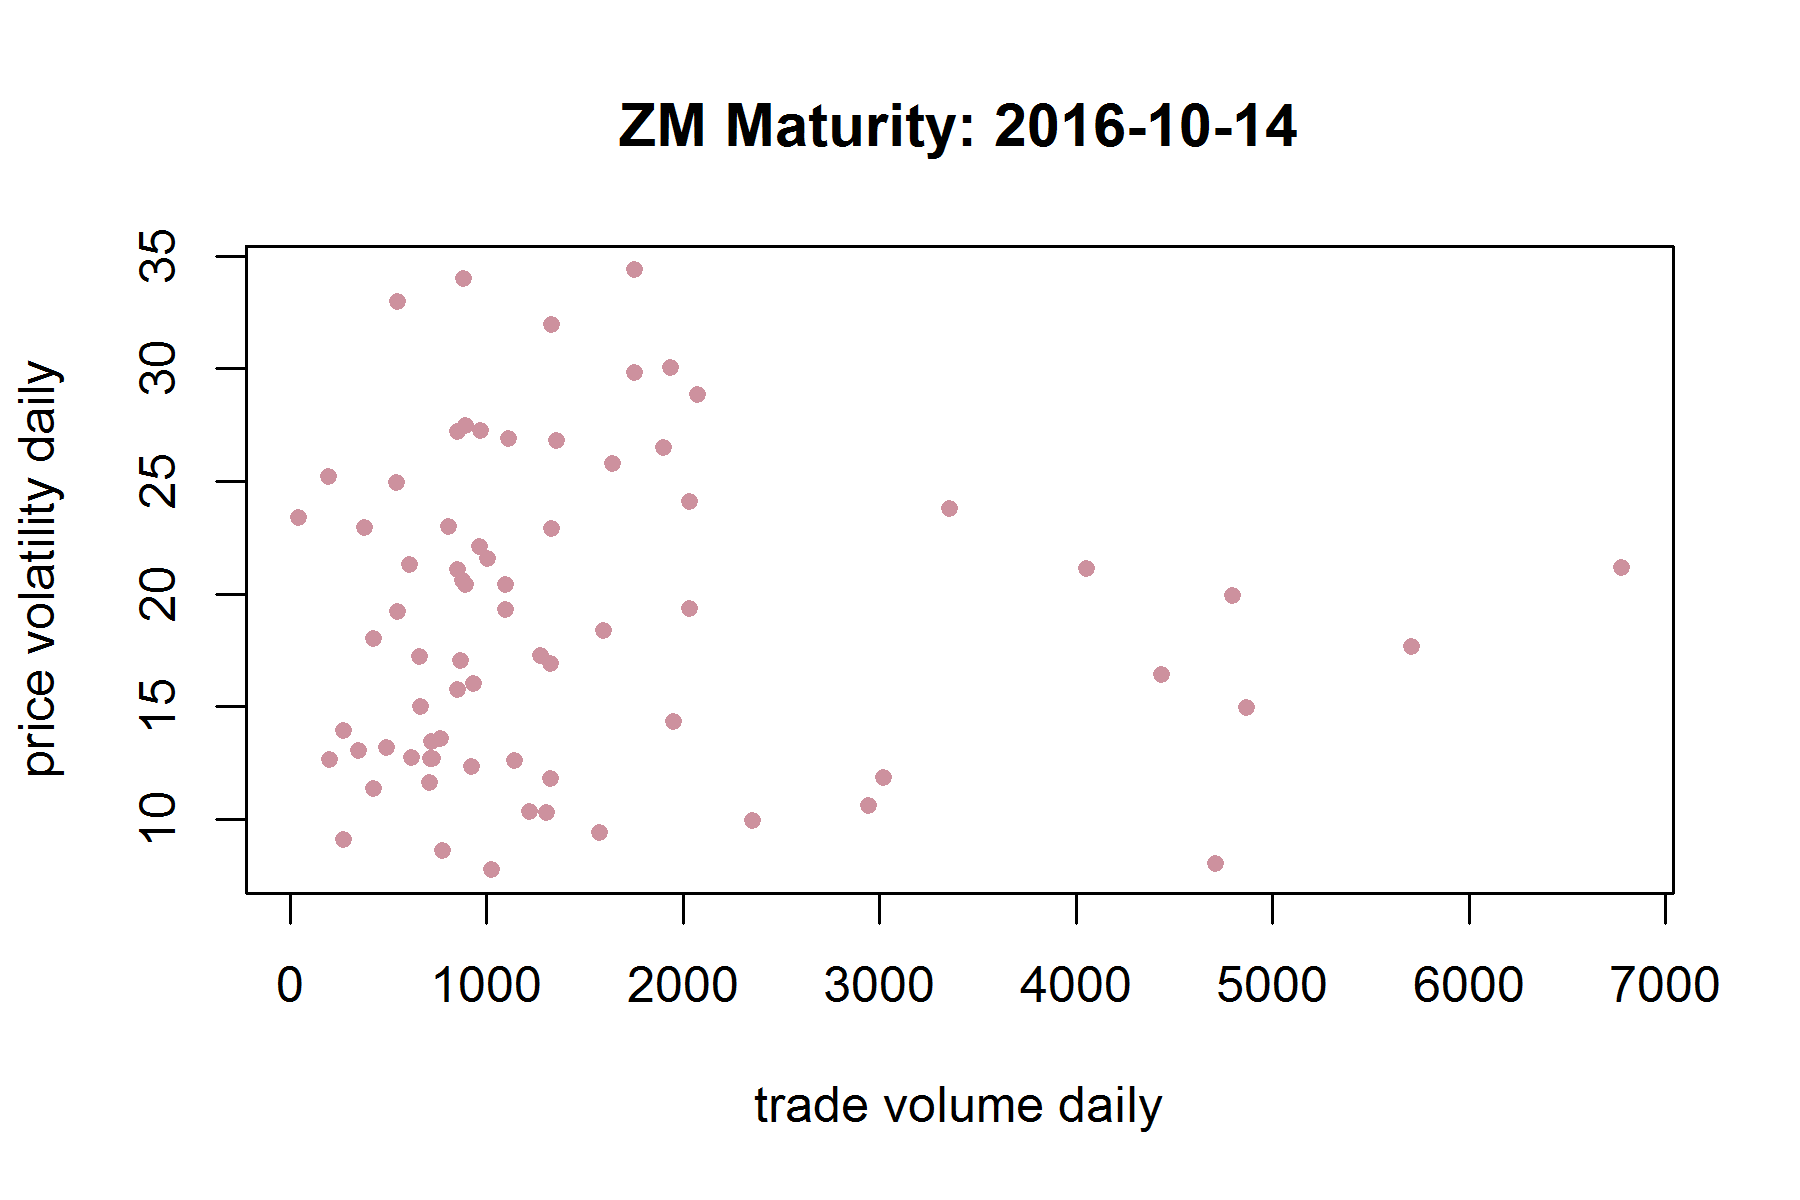
\includegraphics[width=8cm]{ZM2016-10-14daily.png} \\
		\end{tabular}
	\end{center}
	\caption{Price volatility vs. trade volume may show negative correlation cluster}
	\label{fig: 16}
\end{figure}


\begin{figure}[H]
	\begin{center}
		\begin{tabular}{ll}
			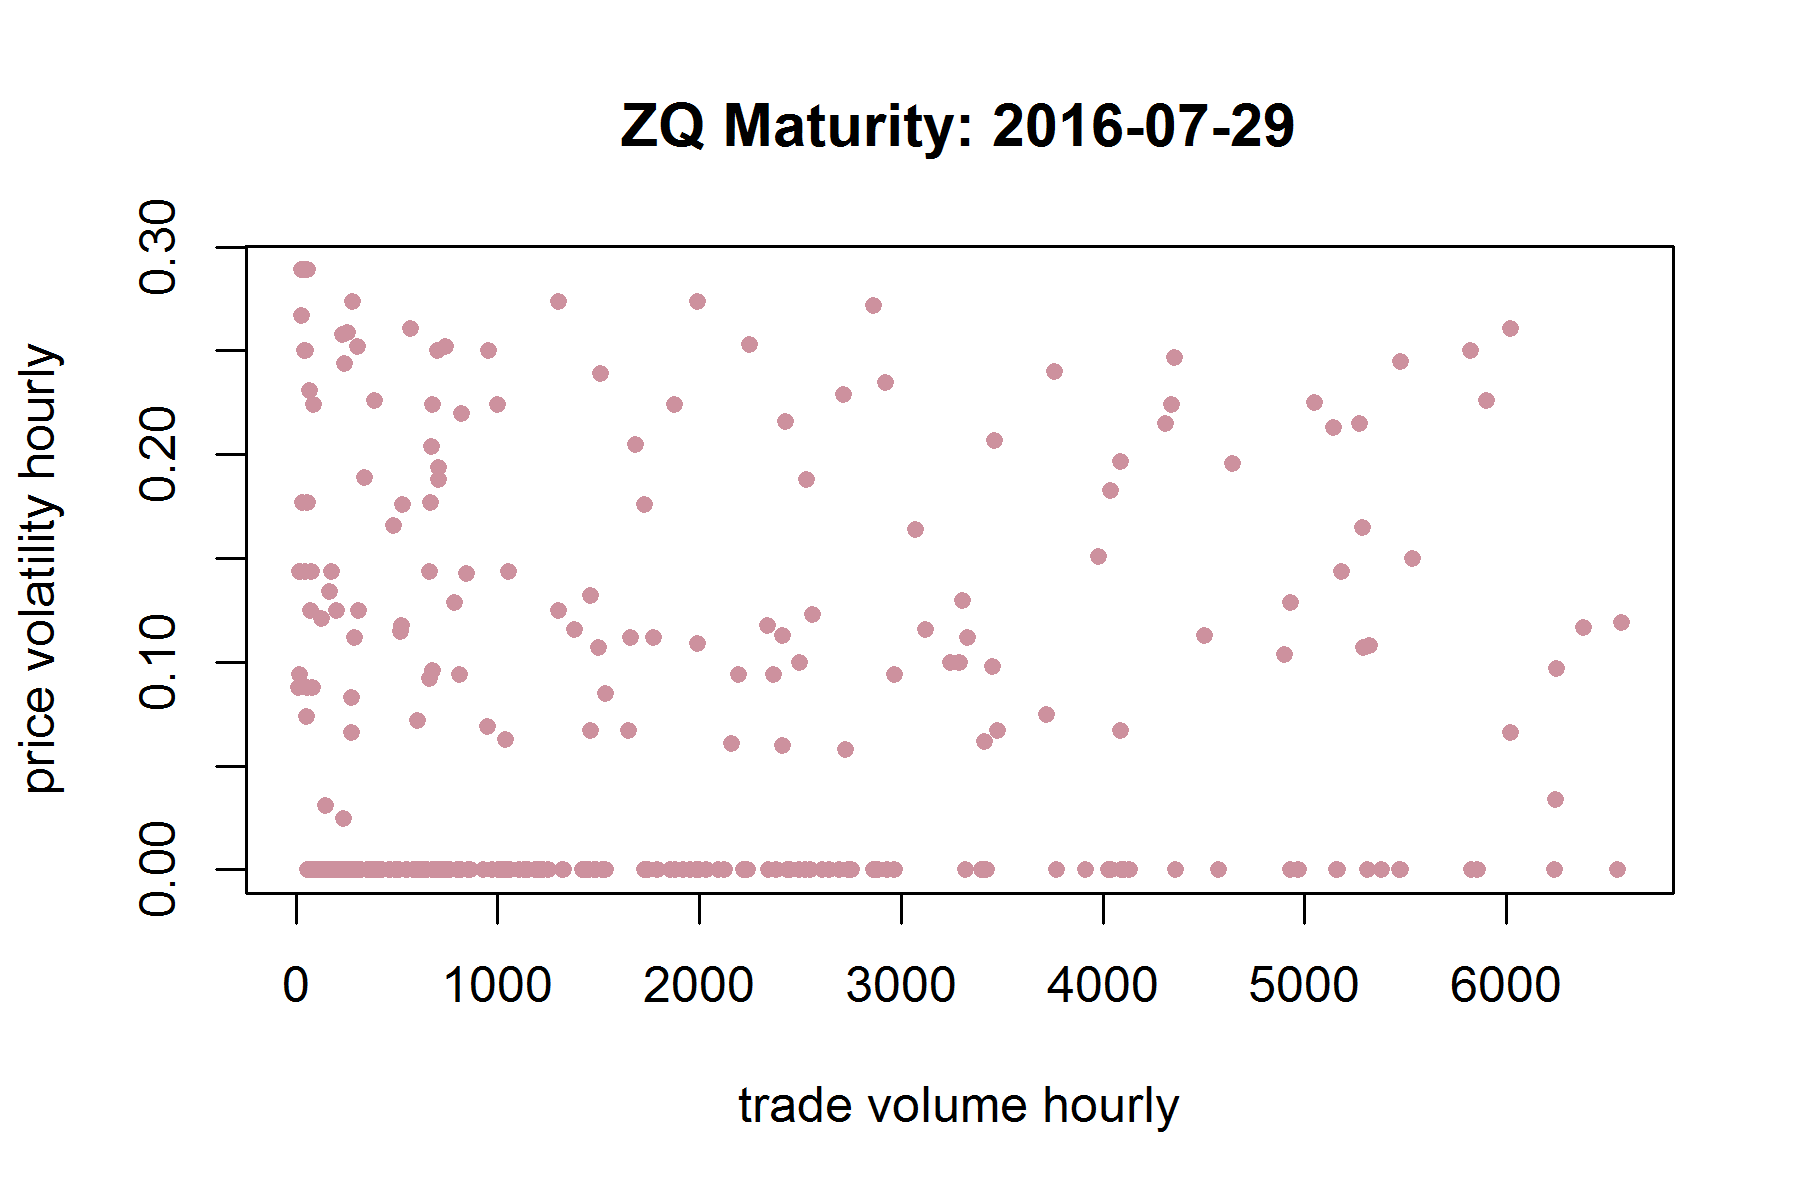
\includegraphics[width=8cm]{ZQ2016-07-29hourly.png} &
			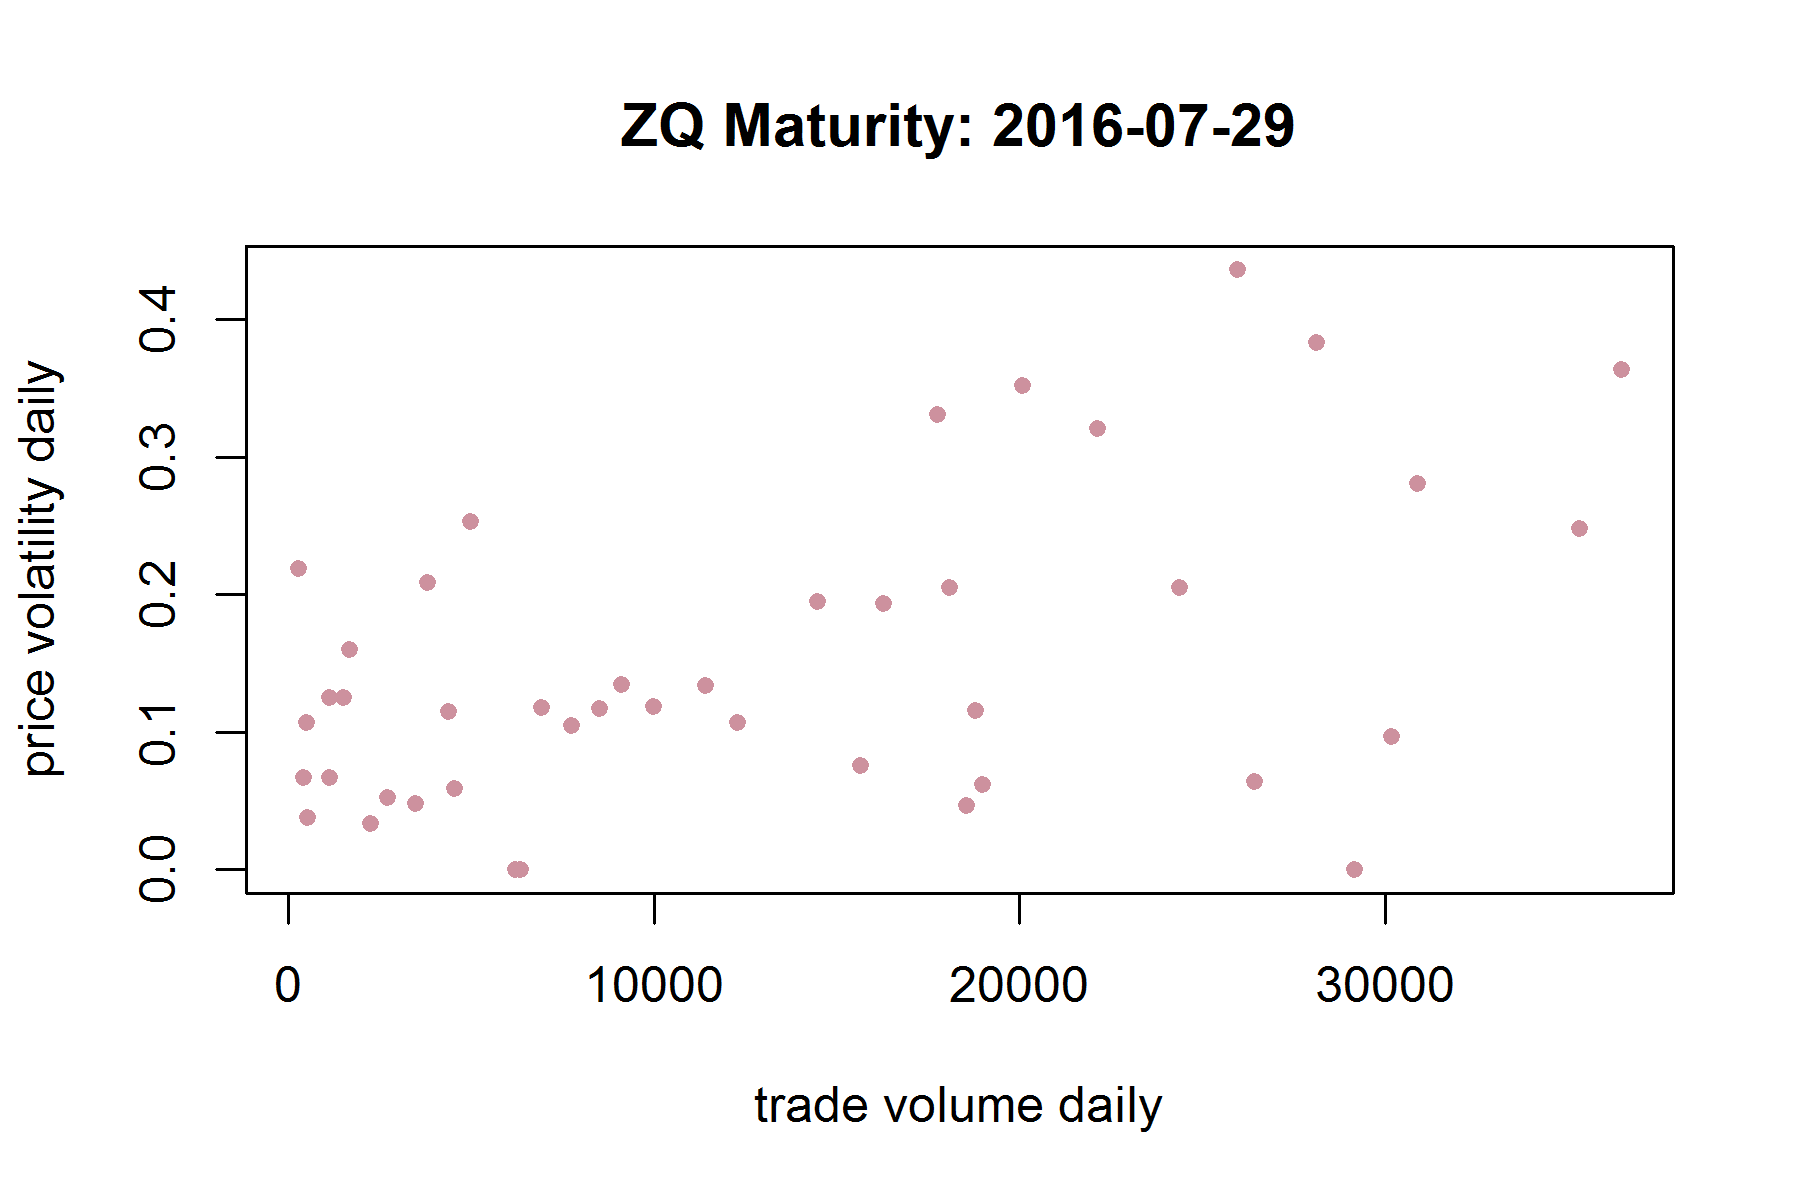
\includegraphics[width=8cm]{ZQ2016-07-29daily.png} \\
		\end{tabular}
	\end{center}
	\caption{Price volatility vs. trade volume hourly shows three clusters}
	\label{fig: 17}
\end{figure}


\section*{Discussion} 
\addcontentsline{toc}{section}{Discussion}
%products with lowest MAD suprising when compared with distributions?
%"relative error" the correct term?
Considering the best model, and comparing MAD to the median, agriculture, energy, and index have relative errors of 0.182, 0.113, and 0.164 respectively but metal, bond, and FX have relative errors of 0.379, 0.254, and 0.301 respectively. This indicates that the regression performs well on agriculture and energy, which was expected since their trade volumes are normally distributed. Surprisingly, the regression does not perform well on the bond market, but performs well on index even though bond trade volume is more normally distributed than index trade volume. Referring to Figure 5, regression is better for index because all the index instruments are similar but the bond instruments are not.

For instance, in the bond market, the 30 Day Fed Fund (ZQ) is much different than the other instruments. This is because the rest are long term bonds of two or more years. It is reasonable that a 30 day bond should behave differently than a long term bond simply because the time frames are so different. The time to maturity spline curve for bond serves as reinforcement of the differences given that the curve begins to rise sharply around 150 days instead of staying low as anticipated. The upward trend is due to the effect of ZQ, as 150 days is where it begins to deviate from the other instruments. Proper modeling should separate ZQ from other bonds. 

Regression also performs poorly on FX which was expected due to lack of normality. In addition, Figure 5 shows heterogeneity within the FX market. Euro (6E) and Eurodollar (GE) behave completely differently. Upon closer inspection, it seems 6E has the shape of an index, as the shape of the curve is in line with the index market. So improvement to this work may be to model 6E as an index.

Finally, regression performs the worst for metal. In Figure 5, silver and gold appear to behave very differently. In particular, the bottom cluster seems to follow a periodic trend whereas for gold the trade volume curve has in inverted parabolic shape.

%instrument level analysis?
When we look at the regression results at the instrument level, the relative error is under .20 for most instruments. The exceptions are both metals (GC and SI) as on the market level, both FX instruments (6E and GE)  as on the market level, and three bonds: 30 Day Fed Fund (ZQ), 30 Yr U.S. Treasury Bond (ZB), and 10Y Treasury Note (ZN). Their relative errors are 0.360, 0.405, 0.2676, 0.459, 0.257, 0.266, and 0.227 respectively. The clustering observed in FX and Metals might be another reason these markets' trade volume are not predicted well. It is reasonable to separate trades into small and large volumes before doing regression. Looking at the bond instruments, the poor performance of ZQ is not shocking for aforementioned reasons. Neither is the poor performance of ZN since it has the highest trading volume. ZB is mysterious, as it appears to behave similarly to ZT. Any future work should analyze this further.

Thus it can be concluded that similarity of instruments being modeled is more important for prediction than normality of distribution for a large number of observations. Therefore instruments similar to one another should be modeled jointly. Models should not be created simply based on market. 

%discuss model coefficients for just best model, model 2, as opposed to all 14.

The model coefficients are also in line with the volumes depicted in visualizations. For instance the coefficient for silver is smaller than gold. The model coefficients also indicate that day of week is not significant. Day of month does seem significant, although it is not as pronounced as time to maturity in most cases. Furthermore, the day of month spline curves reinforce patterns seen in the exploratory analysis visualizations of essentially constant daily trade volume as well as anticipated periodicity, but show a dip around day 8 of 30 for all markets with the exception of FX. Future work should investigate what happens to a product after the first week of trading and why FX is not affected.

%price vola/trade vol rela

%correlation consistent?
%look at trade volume plots for 5 significant to see if close to matu or too far playing a role

Regarding the significant products which do not show constant daily correlation, it is possible that the selection of high volume trading by including observations within the 60th to 90th percentiles was not sufficient and so effects of low volume trading in the nascent and near maturity periods may be present. To find out if this theory is true, the trade volumes were plotted in Figure 18.

All five products have high volume regions selected with ZQ and 5 year treasury note (ZF) showing idealized pattern of dense population above zero, as in Figures 6 and 7. Moreover, none of the products manifest a sharp increase, which typically delineates low and high volumes. We can safely exclude the effects of nascent and near maturity periods from all but Rbob gasoline (RB) since the selected area of this product is still very close to maturity. So non-constant correlation significance is legitimate for ZQ, mini Dow Jones index (YM), heating oil (HO), and ZF implying that these products price volatilities will not be well predicted by trade volume over time because their correlation does not remain constant. Despite this, it would be better to analytically determine the volume inflection point rather than using percentiles. Due to time considerations, the latter was done.

%comment on price vol vs trade vol plots sele
Aside from constant correlation over time, strong correlation between trade volume and price volatility is also needed for predicting price volatility, preferably above .5 in absolute value. Returning to Figures 11 through 17, for most products the daily correlations are stronger and less noisy than the hourly correlations. In some cases 

\begin{figure}[H]
	\begin{center}
		\begin{tabular}{ll}
			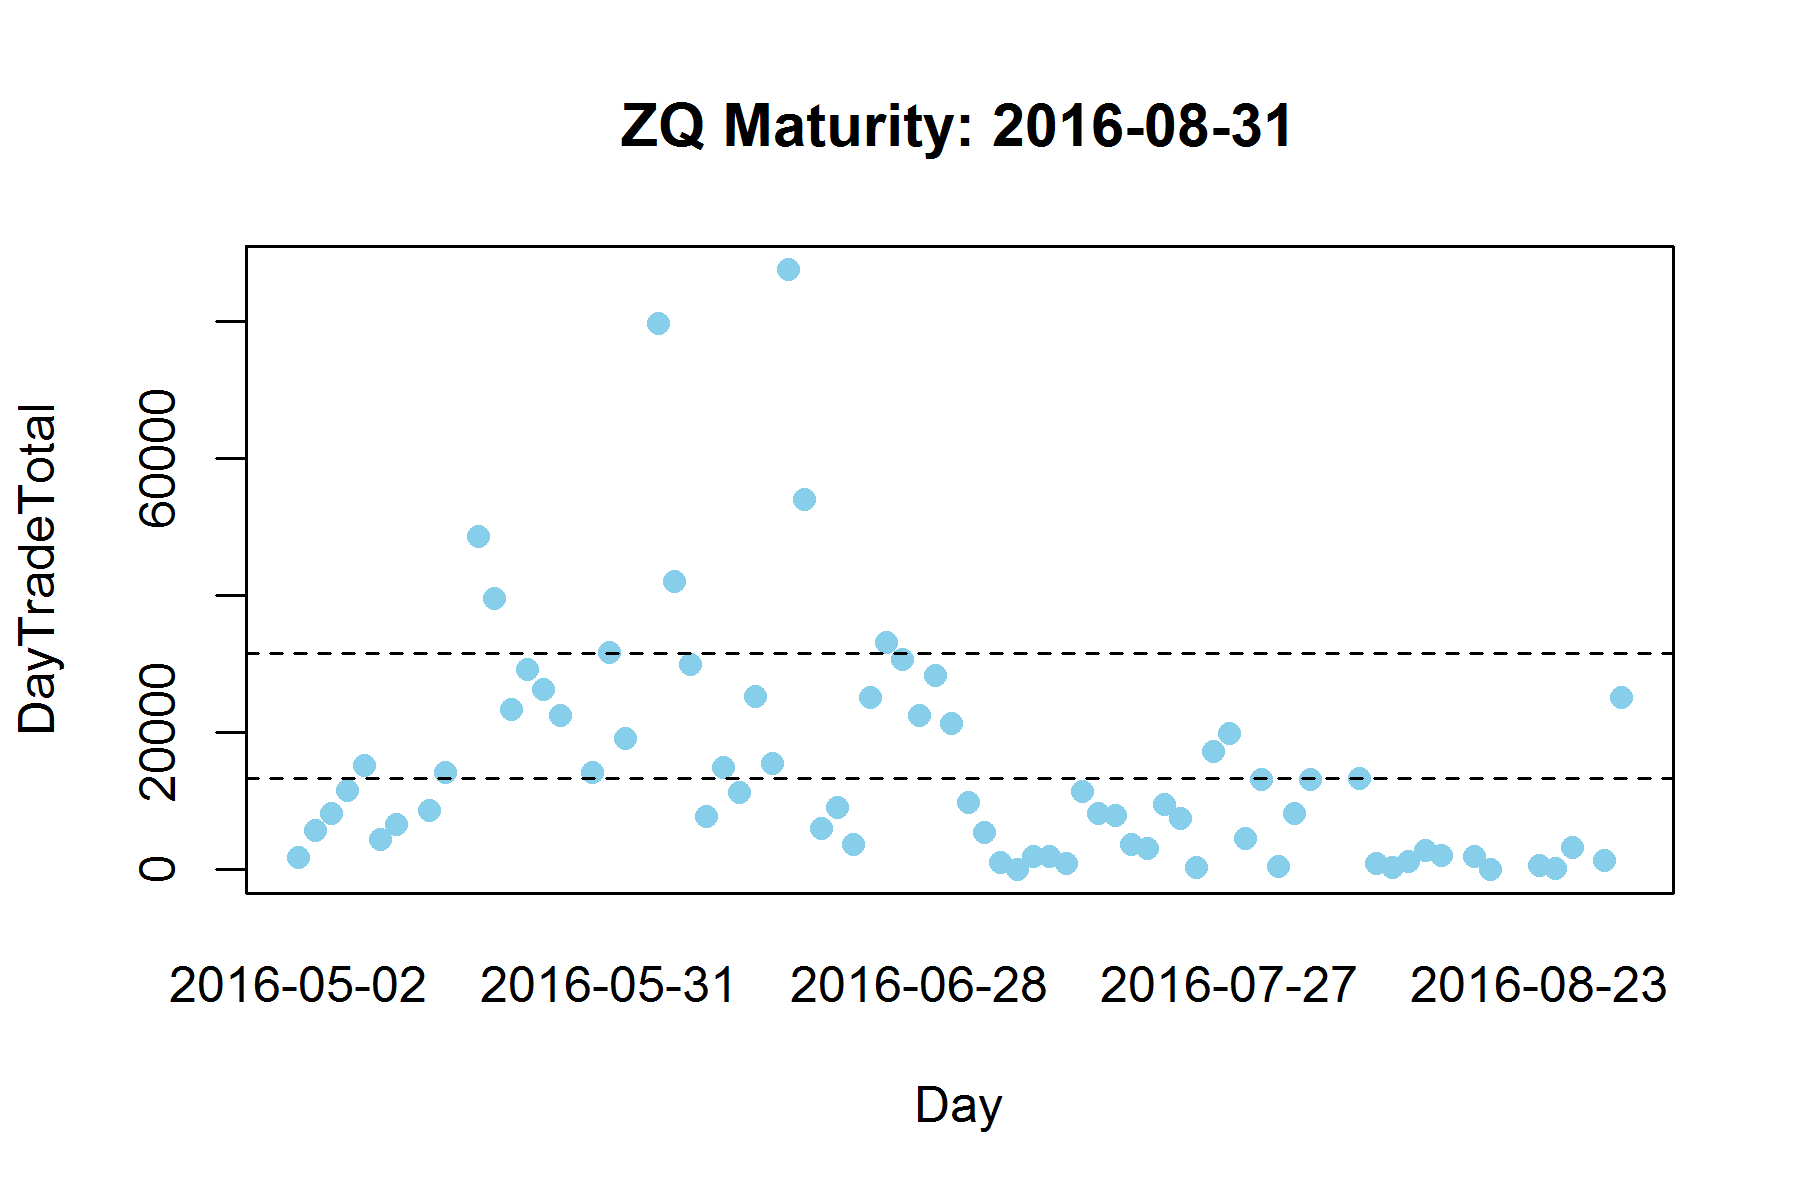
\includegraphics[width=8cm]{ZQtradevolumeTrim.png} &
			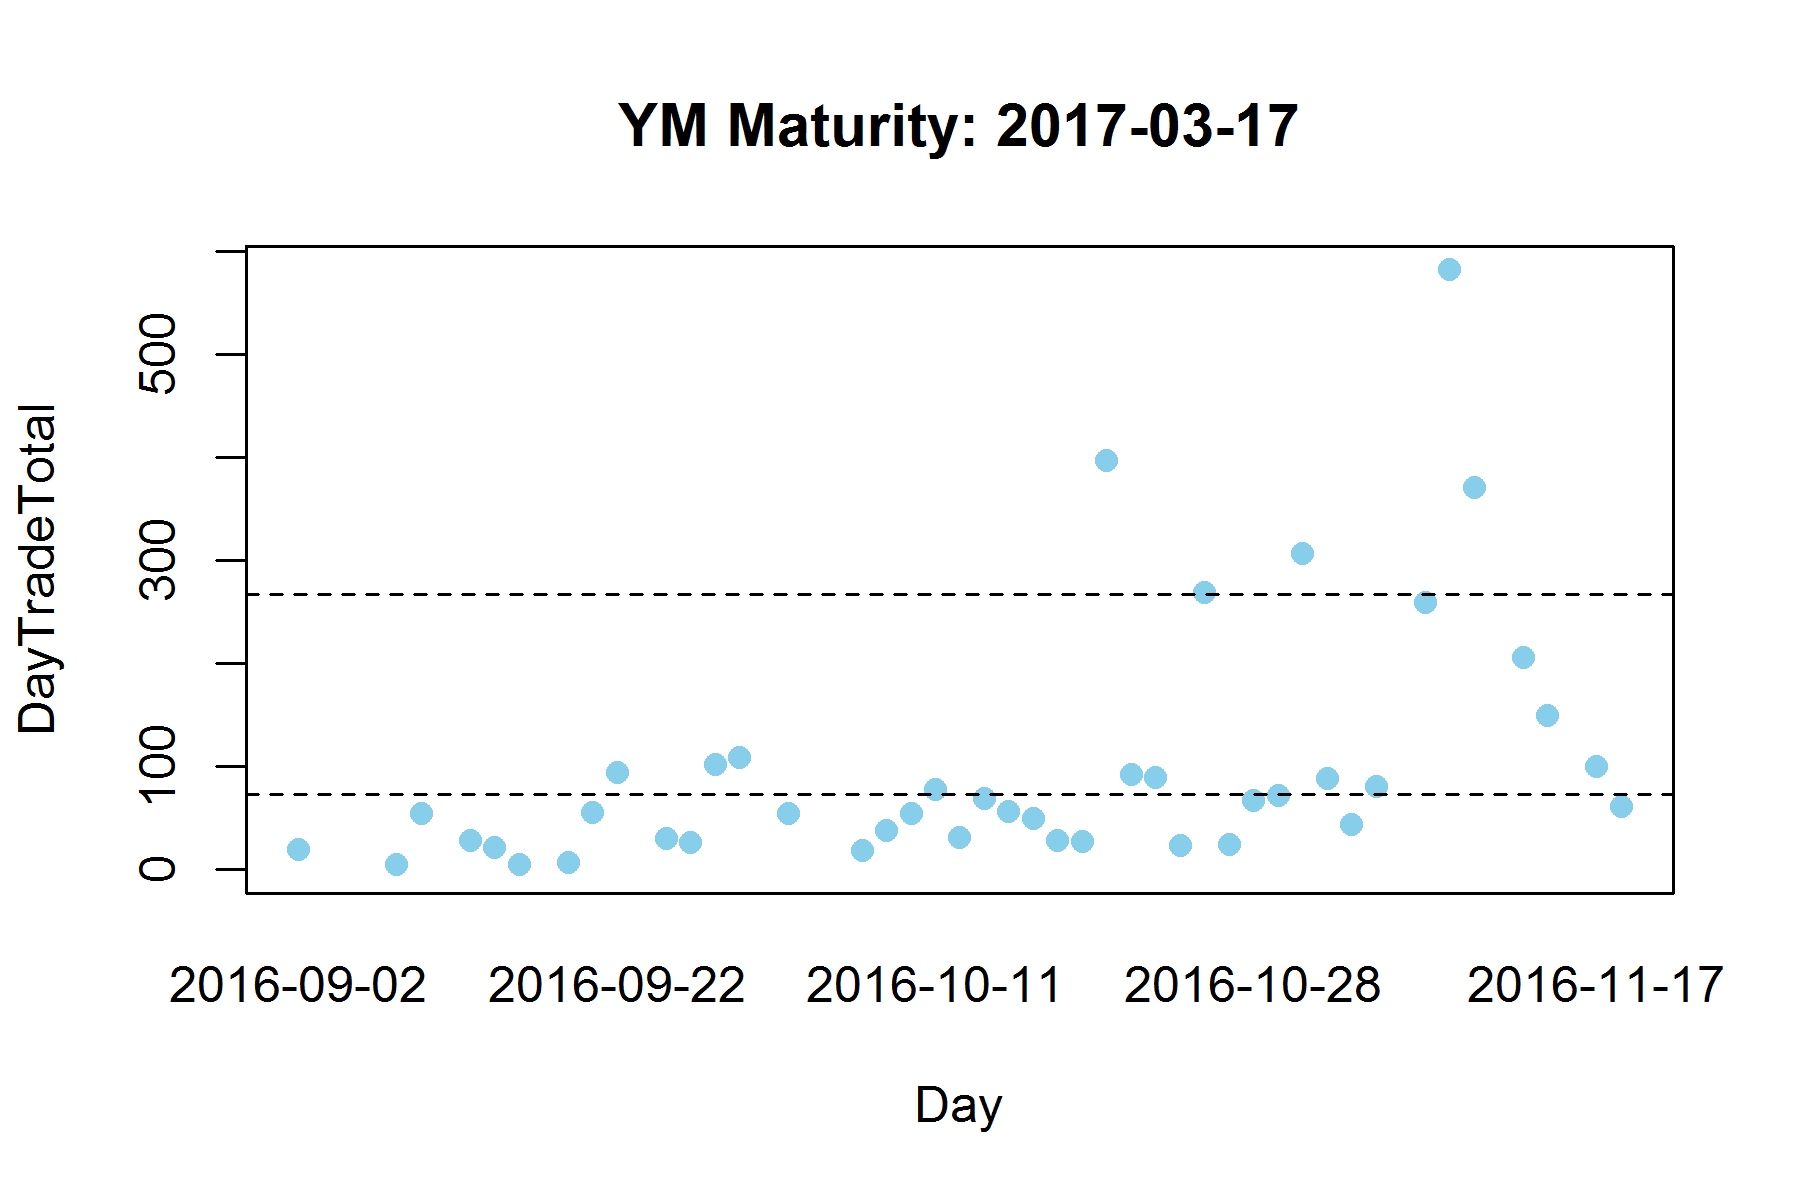
\includegraphics[width=8cm]{YMtradevolumeTrim.png}\\ 
			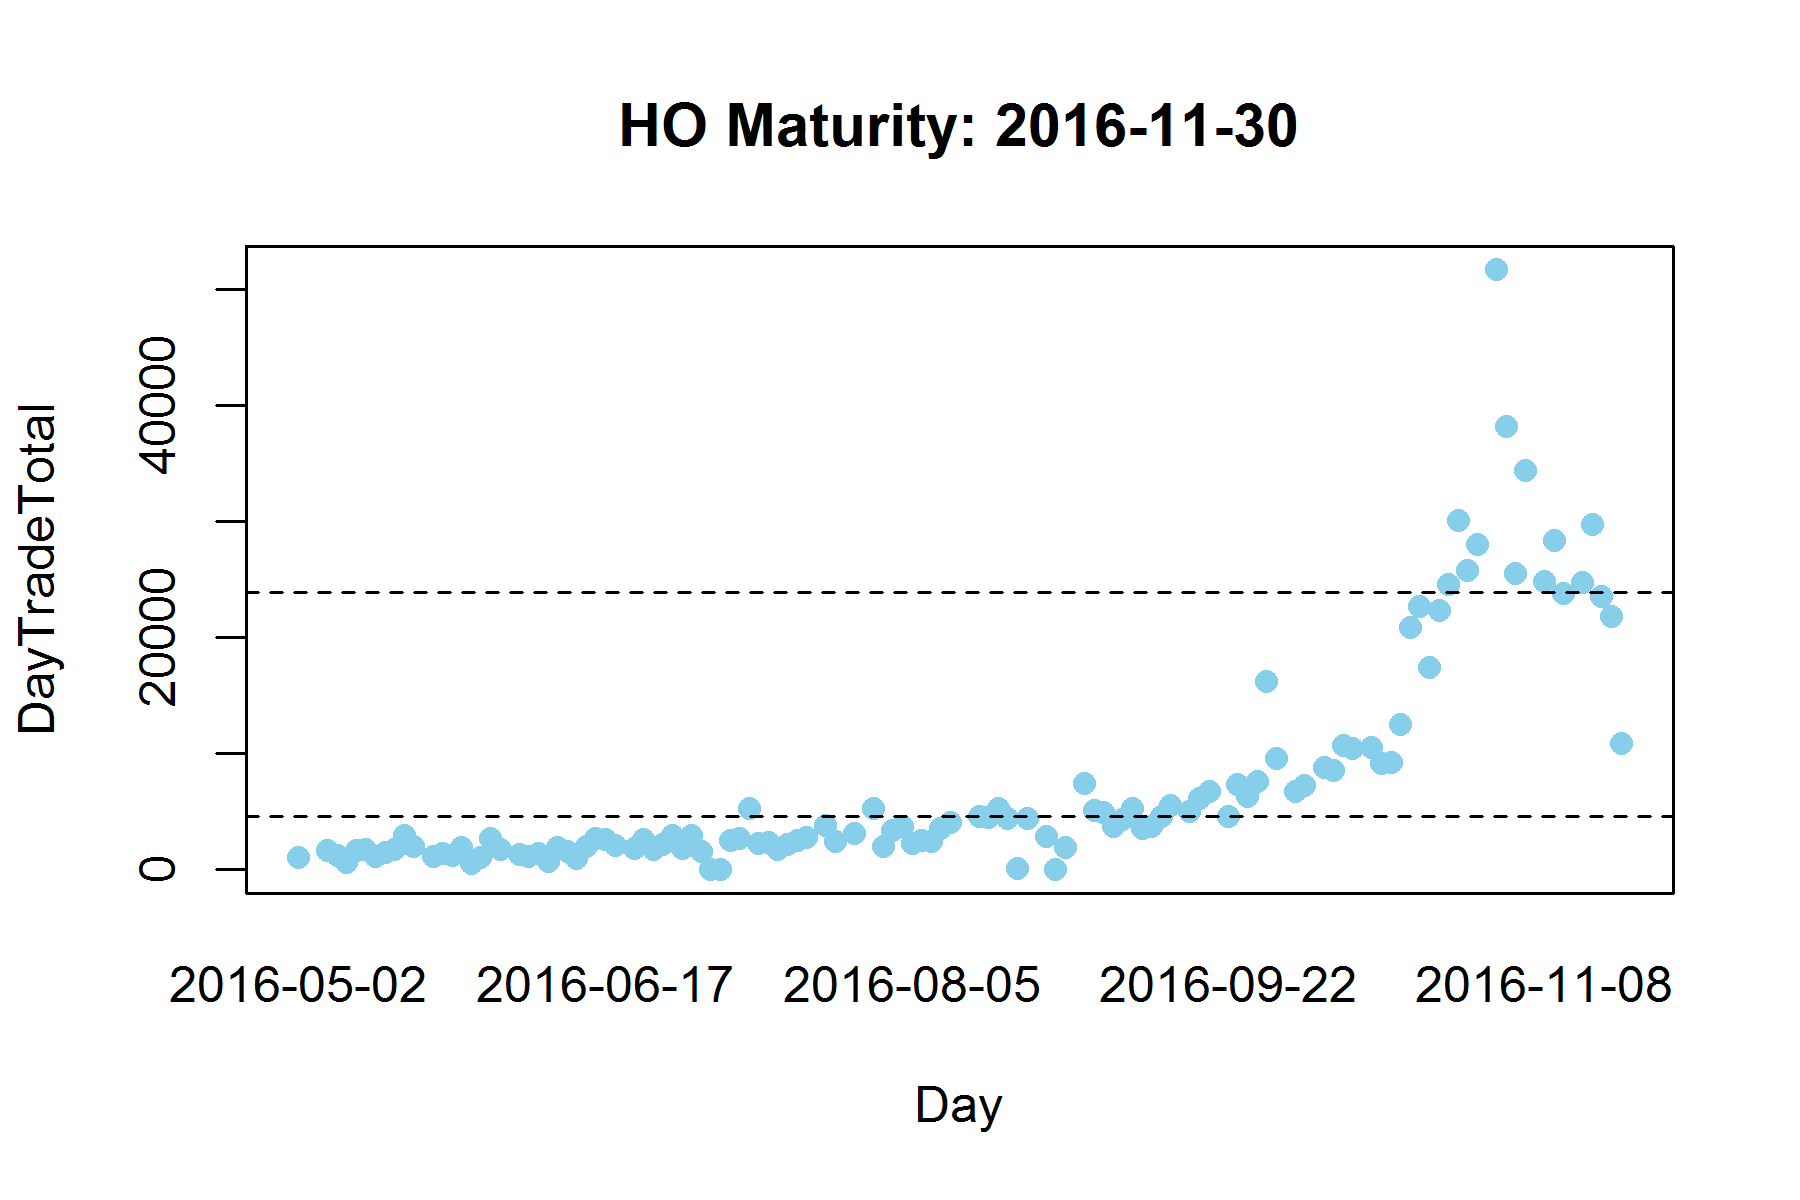
\includegraphics[width=8cm]{HOtradevolumeTrim.png} &
			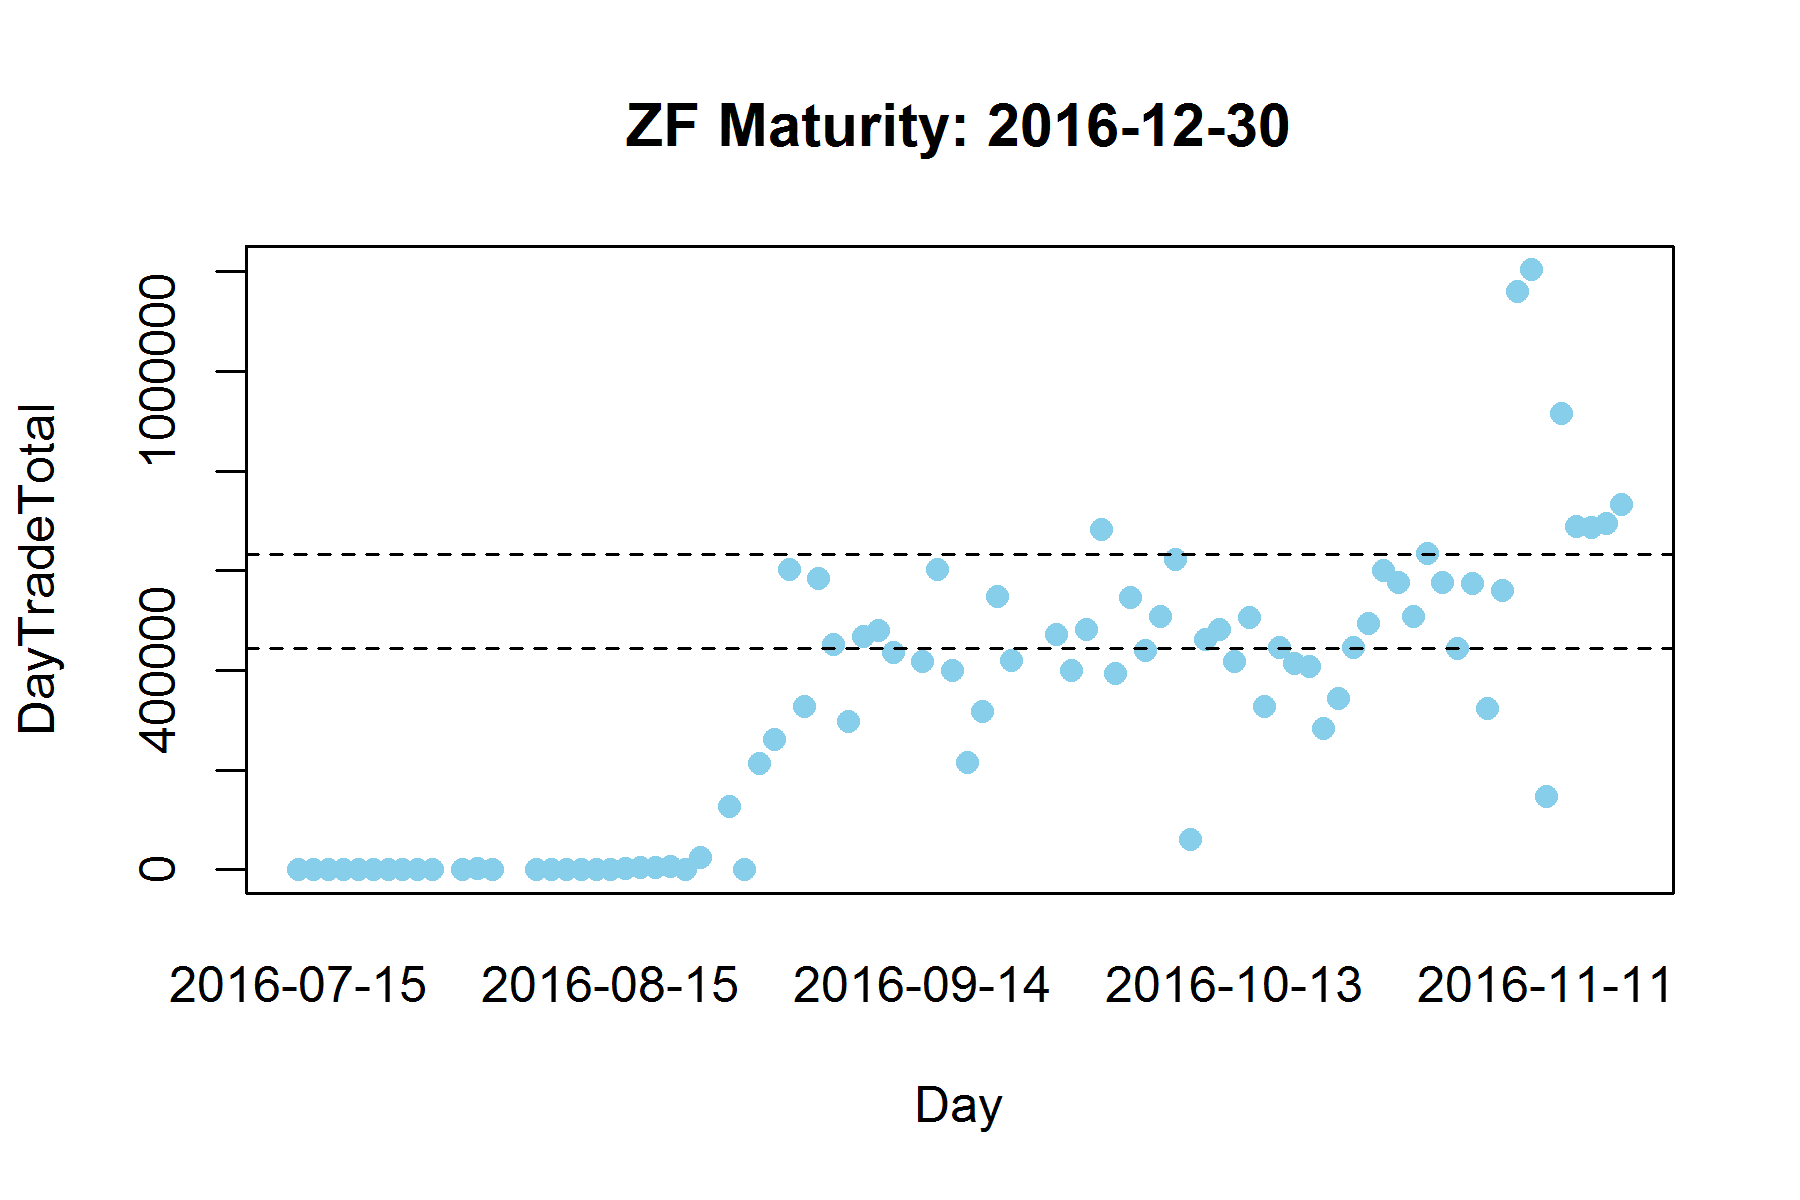
\includegraphics[width=8cm]{ZFtradevolumeTrim.png}\\
			\multicolumn{2}{c}{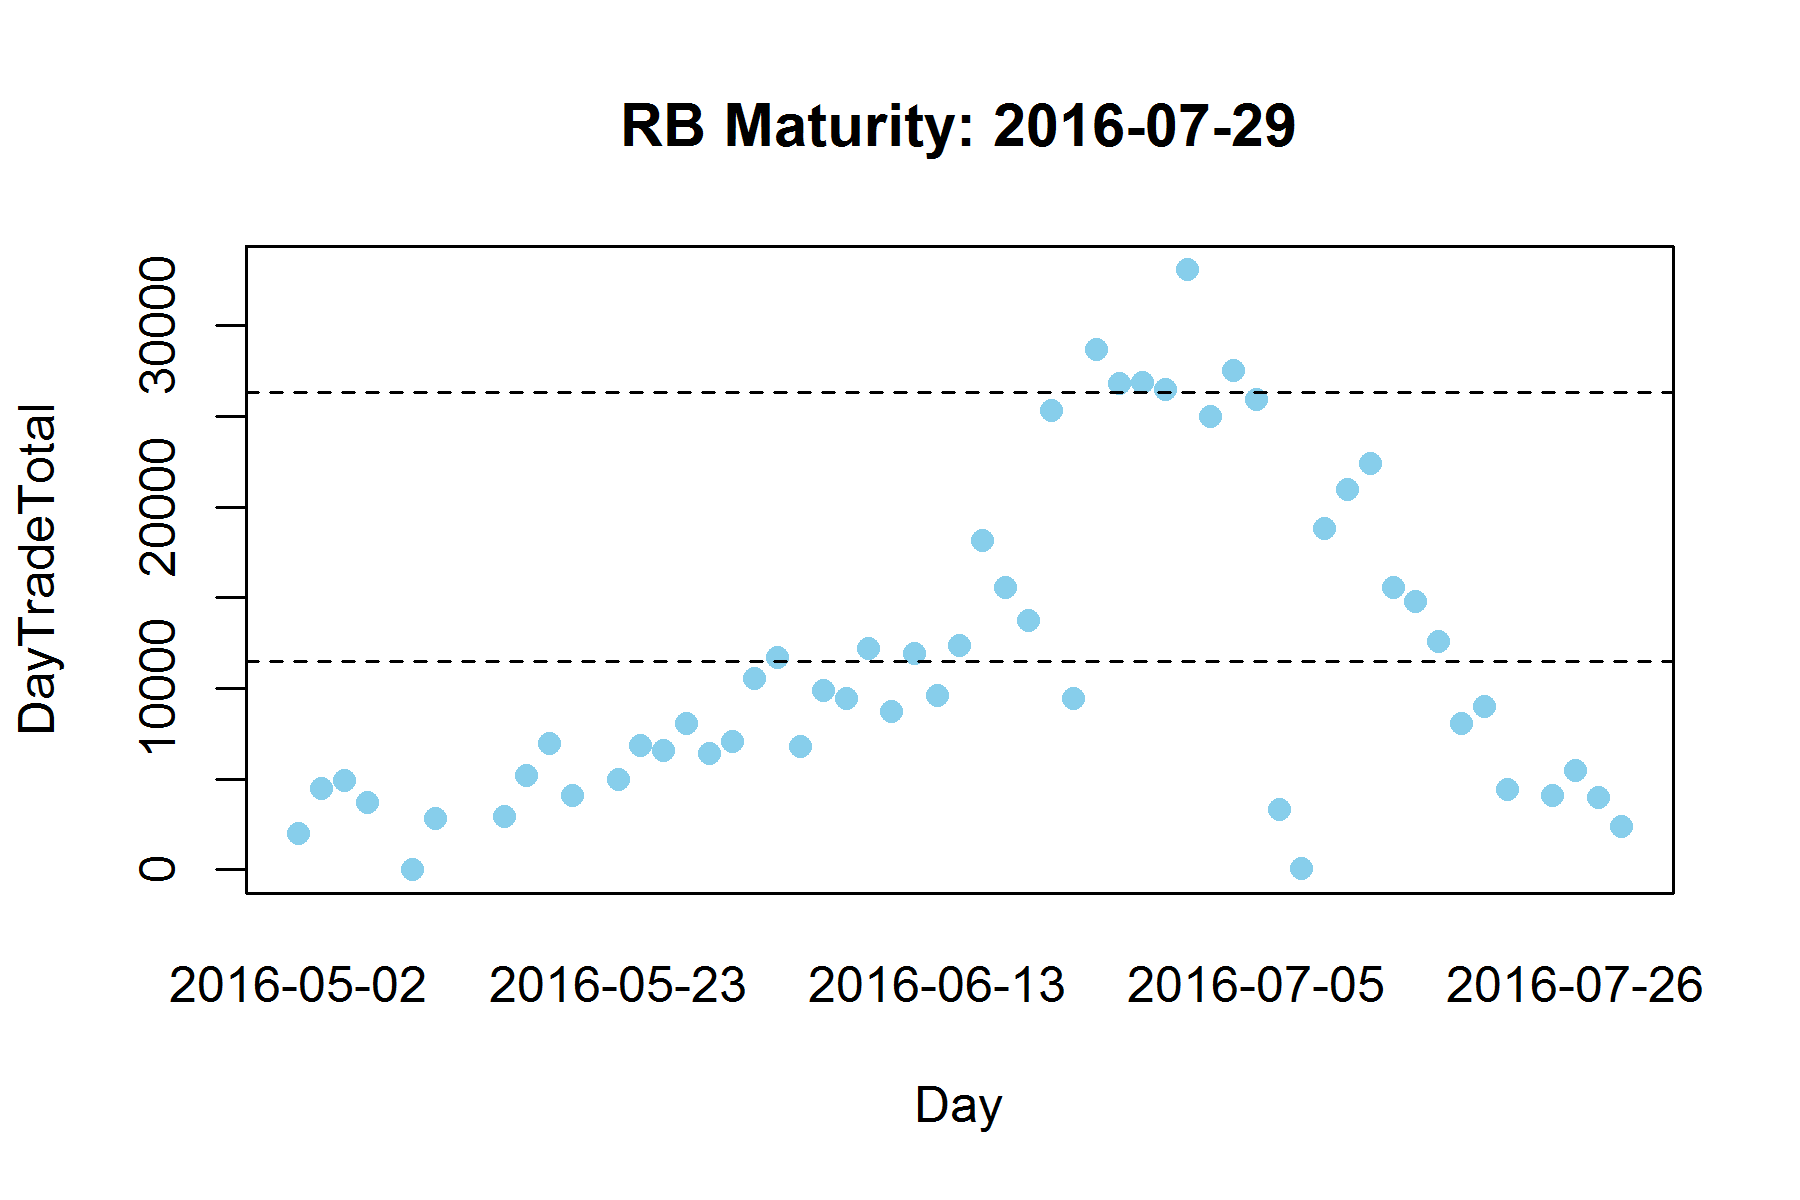
\includegraphics[width=8cm]{RBtradevolumeTrim.png}}
		\end{tabular}
	\end{center}
	\caption{Volume plots for significant products, dashes denote 60th-90th percentiles}
	\label{fig:18}
\end{figure}

\noindent where there is clustering, such as Kc Hrw wheat (KE), ZB, and soybean meal (ZM), observations should be partitioned into low and high volumes before taking correlations into account for price prediction. For agriculture instruments seasonality and temperature most likely play a part in the trade volume clustering observed.

%conclusion
\
\section*{Conclusion}
\addcontentsline{toc}{section}{Conclusion}
It has been shown that Apache Spark is an efficient way to process massive data sets. Here a one node cluster was used, but a multi-node setup is recommended for increasing processing cores and available memory, which in turn improves compute speed. As well, it has been demonstrated that using a penalized regression spline is an effective way of predicting trade volume granted products are similar and we have large set of data to fit models. The covariates most indicative of trade volume are time to maturity and instrument name. Thus, penalized regression splines are a useful for tasks such as building trading algorithms, improving traders' effectiveness, and controlling trading risk. The work here has also explored the viability of predicting price volatility from trade volume by concluding that in the majority of cases, as long as forecasting is made over a trade's active period, correlations observed are constant over time. 

Finally, this study bolsters previous research which states that there is a positive correlation between trade volume and price volatility, validating theory behind speculator and hedger behavior. In cases of product seasonality, it has been revealed that clusters exist and negative correlations may be seen for trades maturing in six or more months in the future. Furthermore, this work shows that positive correlation between trade volume and price volatility is not maintained across all time increments. In particular, positive correlation is mainly observed in measurements made daily, but for the same product, the correlation is not necessarily observed hourly. The information here provides new insight regarding the relationship between trade volume and price volatility, serving to advance regulatory decisions on futures markets. It is hoped that the conclusions stated will inspire other researchers to delve further into the questions raised here and the study of futures markets in general. 
%observe negative correlations when trade 6 or more months from maturity
\newpage

\singlespacing
\section*{Appendices} %additional resources?
\addcontentsline{toc}{section}{Appendices}
\appendix
\renewcommand\thesubsection{\thesection\Alph{subsection}:}
	\subsection{Spark/python code for raw data generation} 
		\label{app:Code1} 
		\lstinputlisting[language=Python]{rawDataGen.py}
		\newpage	
	\subsection{Spark/python code for creating datasets to be analyzed} 
		\label{app:Code2}
		\lstinputlisting[language=Python]{DataGen.py}
		\newpage		
	\subsection{Python code for exploratory data analysis} 
		\label{app:Code3}
		\lstinputlisting[language=Python]{exploratoryDataAnalysis.py}
		\newpage		
	\subsection{R code for spline regression for trade volume}
	 	\label{app:Code4}
	 	\lstinputlisting[language=R]{tradeCountRegression.R}
	 	\newpage	 	
	\subsection{R code for price volatility and trade volume relationship} 
		\label{app:Code5}
		\lstinputlisting[language=R]{PriceVSvolume.R}
		\newpage

\section*{Bibliography}
\renewcommand{\bibsection}{}
\addcontentsline{toc}{section}{Bibliography}
\bibliographystyle{plain}
\bibliography{example}
\newpage

\doublespacing
\section*{Curriculum Vitae}
\addcontentsline{toc}{section}{Curriculum Vitae}
Aniver Bosede was born in Lagos, Nigeria on July 2nd, 1989. In the summer of 2010 she was a National Institute of Health Biostatistics trainee at the University of Wisconsin - Madison. She went on to earn her Bachelor's in Mathematics in 2011 from the University of Pennsylvania, and in 2013 work as a statistical programmer in the division of Biostatistics and Epidemiology at Weill Cornell Medical College. She then received her Master's in Applied Mathematics and Statistics from Johns Hopkins University in 2017. As part of her Master's degree she taught R programming and computational medicine. Aniver is currently a Senior Machine Learning Engineer at Capital One's Center for Machine Learning. Her research interests include statistical analysis on massive data and cluster computing.

\end{document}